\documentclass[10pt,a4paper]{scrreprt}
%page setup
\setcounter{tocdepth}{1}
\usepackage[top=1in, bottom=1in, left=1.5in,right=1in]{geometry}
%generate pdf
\usepackage[pdftex]{graphicx}
%links in Contents
\usepackage[bookmarks, colorlinks=false]{hyperref} 
%embedding pdf
\usepackage[final]{pdfpages} 
%font = times new roman
\usepackage{pslatex}
\usepackage[english]{babel}
\usepackage{enumitem}
\usepackage{listings}
\lstset{basicstyle=\ttfamily,breaklines=true}
\lstset{framextopmargin=5pt,frame=bottomline}
%title and section styling
\usepackage{titlesec}
\usepackage{sectsty}
%For the header and footer
\usepackage{fancyhdr}
\fancypagestyle{plain}{
	%\fancyhf{} % clear all header and footer fields
	\fancyfoot[L]{Department of Computer Engg.}
	\fancyfoot[R]{\thepage}
	\renewcommand{\headrulewidth}{0.4pt}
	\renewcommand{\footrulewidth}{0.4pt} 	}
%header - Project title
\rhead{Kwest : A Semantically Tagged Virtual File System}
\lhead{}
%footer on every page
\fancyfoot[LO,LE]{Department of Computer Engg.}
\cfoot{}
\fancyfoot[RO, RE]{\thepage}
\renewcommand{\headrulewidth}{0.4pt}
\renewcommand{\footrulewidth}{0.4pt}
%page of Contents - title alignment
%set contents title
\renewcommand{\contentsname}{\begin{center}\textsc{Contents}\end{center}} 
\renewcommand{\chapterheadstartvskip}{\vspace*{-\baselineskip }}
\titleformat{\chapter}[display]
	{\normalfont\Large\bfseries\centering}
	{\chaptertitlename\thechapter}{12pt}{\LARGE}
	\titlespacing*{\chapter}{0pt}{0pt}{15pt}
	\chapterfont{\raggedleft}
%add Bib to chapter list with chapter name
\usepackage{natbib}
\renewcommand{\bibsection}{\chapter{BIBLIOGRAPHY}}
%justification awesome set :)
\usepackage[tracking=true,kerning=true,spacing=true]{microtype}
%page clearence for sections
%Latex does this by default 
%EXPERIMENTAL STUFF
\setkomafont{subsubsection}{\large}
%--------------------------------------------------------------------------------------------------------

%--------------------------------------------------------------------------------------------------------
%--------------------------------------------------------------------------------------------------------
\begin{document}
%remove hyphenation
\hyphenpenalty = 100000
\pretolerance = 100000

\begin{center}
\thispagestyle{empty}
\vspace*{4\baselineskip}
\LARGE{\textbf{ABSTRACT}}\\[1.0cm]
\end{center}
\thispagestyle{empty}
\large{{The limitation of data representation in today's file systems is that data representation is bound only in a single way of hierarchically organising files. A semantic file system provides addressing and querying based on the content rather than storage location. Semantic tagging is a new way to organise files by using tags in place of directories.  In traditional file systems, symbolic links become non-existent when file paths are changed. Assigning multiple tags to each file ensures that the file is linked to several virtual directories based on its content. By providing semantic access to information, users can organise files in a more intuitive way. In this way, the same file can be accessed through more than one virtual directory. The metadata and linkages for tagging are stored in a relational database which is invisible to the user. This allows efficient searching based on context rather than keywords. The classification of files into various ontologies can be done by the user manually or through automated rules. For certain files types, tags can be suggested by analysing the contents of files. The system would be modular in design to allow customisation while retaining a flexible and stable structure. \\[1cm]}}
Keywords : virtual file system, semantics, indexing, classification, database, tagging, information access, metadata

\pagenumbering{roman} %numbering before main content starts
%To reset the Header & Footer for TOC and LOF
\pagestyle{empty}

\addtocontents{toc}{\protect\thispagestyle{empty}}

\tableofcontents % adds Index Page

%set alignment for list of figures
%\renewcommand{\chapterheadstartvskip}{\vspace*{-\baselineskip }}
\titleformat{\chapter}[display]
	{\normalfont\Large\bfseries\centering}
	{\chaptertitlename\ \thechapter}{12pt}{\Large}
	\titlespacing*{\chapter}{0pt}{0pt}{15pt}
	\chapterfont{\raggedleft}
\pagestyle{empty}
\addtocontents{lof}{\protect\thispagestyle{empty}}
\listoffigures % adds List of Figures
\listoftables % adds list of tables
\cleardoublepage
%And reset back the settings we choose for Header and Footer
\pagestyle{fancy}
\newpage
\pagenumbering{arabic} %reset numbering to normal for the main content
%reset chapter name alignment
\titleformat{\chapter}[display]
	{\normalfont\Large\bfseries\raggedleft}
	{\chaptertitlename\ \thechapter}{12pt}{\Large}
	\titlespacing*{\chapter}{0pt}{0pt}{20pt}
	\chapterfont{\raggedleft}

%\input{prob_def.tex} % adds the introduction page
%\input{literature.tex} % adds the Literatu	re Survey page
%\chapter{Software Requirement Specification}
\section{Introduction}
\subsection{ Purpose}

[This presents comprehensive description of the intended purpose and environment of KWEST. It fully describes what the KWEST will do and how it will be expected to perform. In addition it also contains non-functional requirements.]

\subsection{ Intended Audience And Reading Suggestion}
The intended audience of this document includes both developers and reviewers of the system.

\subsection{Project Scope}
This project is a virtual file system capable of storing semantics with which it facilitates the finding of relevant information.
\begin{enumerate}
\item  Information is stored in tags, which are extracted from a file's metadata. This
information may be generated implicitly by the system or supplied explicitly by the
user.
\item  The validity of information is based on the users level of organising things.
\item  The system is currently designed to extract metadata from a limited set of popular
file types for audio, video and images and PDF documents.
\item  The modular architecture allows for plugins to be added which can add additional
functionality, and recognition for more file types. This allows the project to be
extended and modified according to the functionality required.
\item  The level of awareness generated by the system is based on the frequency of access
and input provided by the user.
\item  The current implementation is based on the Linux kernel. Future implementations
can be extended to other platforms and devices.
\item  As the system is an virtual entity, it does not need extensive modifications to be
ported to other file systems and operating systems.

\end{enumerate}

\subsection{User Classes And Characteristics} 

The system can be used by three types of users:
\begin{enumerate}
\item General User 

Uses the system without any complex modifications in the system.
\item Advanced User 

Understands the system and creates rules and automation’s based on personal needs.
\item Developer 

Uses the API provided and develops modules that extend the system.
Only advanced users utilise the semantic nature of underlying file system to the fullest.
This does not create any blocks for the general user, who can also use Kwest satisfactorily.
Developers are a different group of users who can extend Kwest through modules. These
modules can modify or define additional behaviour for the system for specific file types.
\end{enumerate}

\subsection{Operating Environment}\begin{enumerate}
\item  Kwest requires FUSE \cite{FUSE} version 2.8.6 and above.

\item Kwest can run on any Linux installation which contains required versions of FUSE.
\item  Furthermore, since kernel version 2.6.14, FUSE has been merged into the
mainstream Linux kernel tree. As a result Kwest can run on any Linux distribution
created from Kernel version 2.6.14 or above.

\item Kwest is a virtual file system mounted to a folder or a loop device.
\item It is the responsibility of the user that mounting and unmounting of the system be
done with standard rules and precaution

\end{enumerate}

\subsection{Design And Implementation Constraints}

Implementation Constraints
\begin{enumerate}
\item Kwest uses FUSE to manage userspace file systems. Hence, access is limited to the
executing userspace for the program.
 \item Since the entire application is executed in userspace only, there cannot be interaction
with the kernel directly.
\item Although Kwest implements a virtual file system which is accessible to all entities,
we have implemented the system with command line as the primary interface. Other
file managers such as Nautilus can only browse but not tag files. This limitation can
be addressed with plugins or additional modules built for the specific file manager.
\item The SQLite database is an integral part of Kwest and is contained in a single file. It
is vital for the system that integrity of the database is maintained.
\end{enumerate}
Design Constraints

\begin{enumerate}

\item Currently, the auto-tagging feature has been limited to common and popular file
types such as audio (mp3, wav, etc.), images (jpeg, png, etc.) and video (mp4, avi,
etc.). This functionality can be extended with modules or through special tools
made specifically for this purpose.

\item The amount of information visible through common file system commands (e.g.
ls - list contents) is a limitation for Kwest. We cannot show tagging information
through these interfaces. Alternate methods for this can be implemented keeping
the end user in mind.
\end{enumerate}


\subsection{ Assumptions And Dependencies}

Assumptions
\begin{enumerate}
\item Users of this software are aware of how semantics are used to categorise
information.
\item Users can recognise or identify appropriate tags in relation to files.
\item It is assumed that the user is well versed in organisation information and uses Kwest
as a tool rather than an assistant.
\item The user has the required privileges / rights to run Kwest and all its operations.
\end{enumerate}
Dependencies

\begin{enumerate}
 \item Kwest uses several external libraries to extract metadata from popular formats for
audio, images etc. TagLib, EXIF etc. which are required at compilation time. These
enable the system to handle metadata extraction for popular file formats.


 \end{enumerate} 


\section{System Features}
\subsection {Tags}
\begin{enumerate}
\item Manual Tagging 

Manual tagging is the basis of semantics in Kwest. The user can assign any tag to the files in Kwest. These tags are then stored internally in a database. The user can create new tags or use tags already defined by the system. Total freedom is given to the user to organise data. Multiple tags can be assigned to the to a single thus allowing its access through multiple locations without duplication of data.
\item Automatic Tagging 

Kwest also features automatic tagging of files. The user can define certain rules under which files will be assigned tags. The system will implement those rules for all files satisfying the defined constraints. This would prevent repetitive tagging operations for the user. 
\item Importing tags 

Certain popular file formats such as mp3, jpeg etc have metadata embedded in them. Kwest supports such popular format and uses this metadata to automatically assign tags to the files. This feature enables the user to collectively classify and store the data under these tags.
\end{enumerate}

\subsection{Database}
\begin{enumerate}
\item Consistency 

Kwest uses an internal database to store and manage data. It is vital that the database always remains consistent. Kwest uses logging mechanisms to ensure that operations on the database always reach an endpoint. 
\item Access 

The database files used by Kwest are not locked down or access restricted. The Kwest API provides facilities that can be used to access the database. However, this feature is made available with the understanding that the integrity of the database will be maintained always.
\end{enumerate}

\subsection{Relation With Existing Data}
\begin{enumerate}
\item Importing semantics 

Users already have certain organisational structures in the way they store data in file systems. Kwest imports these semantics by converting the storage hierarchy to tag-based hierarchy. This allows the entire file system to be imported into Kwest along with the users previous organisation structure. 
\item Files are executable ready 

The files can be directly executed through the virtual file system without making any modification to the files like audio, video files can be played through the virtual system, images can viewed and documents can be opened and read.  
\end{enumerate}

\subsection{Exporting Semantics}
\begin{enumerate}
\item Export file system 

As the entire file system exists as a virtual entity, Kwest provides the export feature. Where the file system can be exported to another system where the data can be imported by another instance of Kwest. 
\item Export tagged files 

It is also possible for the user to export data under certain tags to an external location. The semantic organisation showed by tags is converted to actual directories and files are then copied to these directories. This way the user can export Kwest semantics and data to outside locations.
\end{enumerate}
	
\subsection{Modularity}
\begin{enumerate}
\item Modules As Plugins 

Kwest is an extendable system. It can use external modules to increase functionality or to modify existing operations. Support for using modules is built into Kwest right from the design stage. Additional extraction libraries can be included using the plugin module.
\item Support for developers 

Kwest provides support to developers by providing access to all internal features and database. The API layer allows developers to easily supplement internal operations with their modules.
\end{enumerate}

\section {External Interface Requirements}

\subsection {User Interfaces}
The user can use the system through the command line. The system mounts a virtual file system which the user can use to navigate through. If the file explorer/browser supports virtual file system, the user can use that to navigate through the files. 

\subsection {Hardware Interfaces}
No hardware interfaces used as the file system exists as a virtual entity.

\subsection {Software Interfaces}
\begin{itemize}
\item FUSE\cite{FUSE} \\
Kwest uses FUSE to run the file system code in user space without editing the kernel code.The FUSE module provides only a ``bridge'' to the actual kernel interfaces. Major file system operations are defined by FUSE and forwarded to Kwest for implementation.
\item SQLite\cite{SQLITE} \\
Kwest uses SQLite database to store data. In contrast to other database management systems, SQLite is not a separate process but an integral part of Kwest. Database is accessed and modified for most of the operations performed by Kwest.
\end{itemize}
\subsection {Communication Interfaces}
Kwest can be accessed like any other file system via Command line or file managers like Nautilus, Thunar etc.

\section {Nonfunctional Requirements}

\subsection {Performance Requirements}
\begin {itemize}
\item Response Time \\
The response time for any action on the file system or the database should be reasonable under normal operational circumstances. 
\item Capacity \\
Kwest can be used by any user with sufficient permissions to initialise the filesystem. Subsequent operations like read, write, modify etc. are restricted by user permissions similar to normal file systems.
\item Scalability \\
Kwest provides suggestions and includes automated tagging rules for Audio, Video and Images. It also allows manual tagging of files by the user. Various modules can be further added for recognising and categorising other file types.
\end{itemize}

\subsection {Safety Requirements}
\begin{itemize}
\item Power Failure \\
The system maintains a log file for database. It prevents data corruption by committing data that has been fully written to the log. This should prevent most, if not all, data corruption.
\item Data Loss \\
If any file is accessed which is mentioned in database but deleted from the system then it is removed from the database and appropriate message is displayed to user.
\item Access Rights \\
The system checks if the file tagged is available to user for access. It does not allow files to be included which cannot be access by the user.
\end{itemize}

\subsection {Security Requirements}
Kwest can be used only by a single user with sufficient rights to execute the software. No other user will have permissions to modify tags and files in the system.

\subsection {Software Quality Attributes}
\begin{itemize}
\item Availability \\
The System shall be available from mounting the file system until its unmounted.
\item Updatability \\
The system shall allow for addition or deletion of files under tags.
\item Reliability
\begin{itemize}
\item The system shall save new tags created by active user.
\item The system shall save the file path of an active user to database whenever new files are added to a tag.
\item The system shall maintain a log file which records every operation on database.
\item The system shall modify database whenever tags or files are deleted.
\item The system shall remove file entries from database whenever it is unable to access them.
\end{itemize}
\item Portability \\
The system is implemented on Linux. It is compatible with various other Linux distributions like Ubuntu, Fedora, Red Hat, etc.
\item Testability \\
New modules designed to be added to the system, to identify file types other than audio, video and images must be tested to check if they are compatible with input-output format of the system.
\item Usability \\
The system does not have a large learning curve as the user deals with commands common to all file systems. Documentation provided for the system will include user manuals, developer reference and common FAQ.
\end{itemize}

\section{Other Requirements}
\subsection{Legal Requirements}

All the libraries, programs used in this project are open sourced under GPL. SQLite is a
database which is free to use, distribute or modify. The FUSE kernel module is merged
with the Linux Kernel, which is open sourced and freely available under GPL. There
are no proprietary or closed source products, libraries or interfaces used in this program.
The project Kwest and its subsequent implementations will be open sourced under the
GPL upon completion.

%\newpage
\section {Analysis Model}
\subsection {Data Flow diagram}
\vspace*{1.5cm}
\hspace{6.5cm} \textbf{Level 0} \\


\begin{figure}[H]
\centering
\setlength\fboxsep{0pt}
\setlength\fboxrule{0.5pt}
\fbox{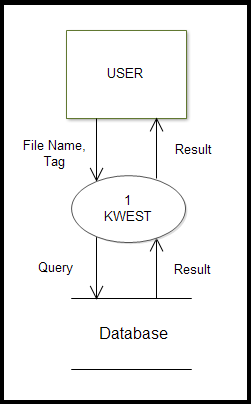
\includegraphics[width=0.5\linewidth]{./diagrams/dfd0.png}}
%\includegraphics[width=0.8\textwidth]{image.png}
\caption{Data flow diagram - Level 0}
\label{fig:dfd0}
\end{figure}

\newpage
\vspace*{2cm}
\hspace{5.5cm} \textbf{Level 1} \\
\begin{figure}[H]
\centering
\setlength\fboxsep{0pt}
\setlength\fboxrule{0.5pt}
\fbox{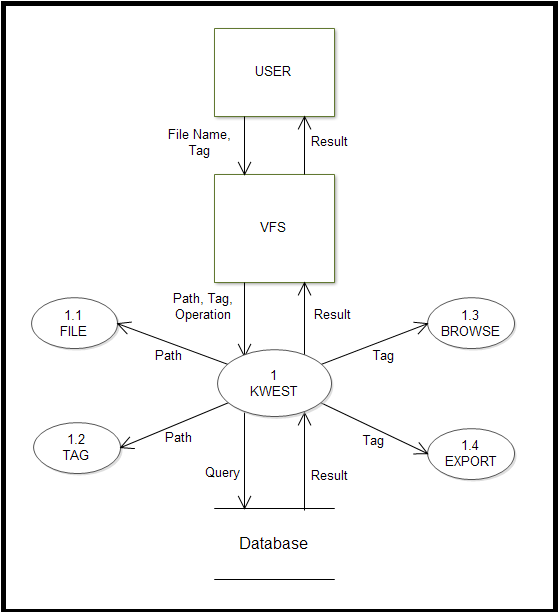
\includegraphics[width=0.9\linewidth]{./diagrams/dfd1.png}}
%\includegraphics[width=0.8\textwidth]{image.png}
\caption{Data flow diagram - Level 1}
\label{fig:dfd1}
\end{figure}

\newpage
\vspace*{2cm}
\hspace{5.5cm} \textbf{Level 2} \\
\begin{figure}[H]
\centering
\setlength\fboxsep{0pt}
\setlength\fboxrule{0.5pt}
\fbox{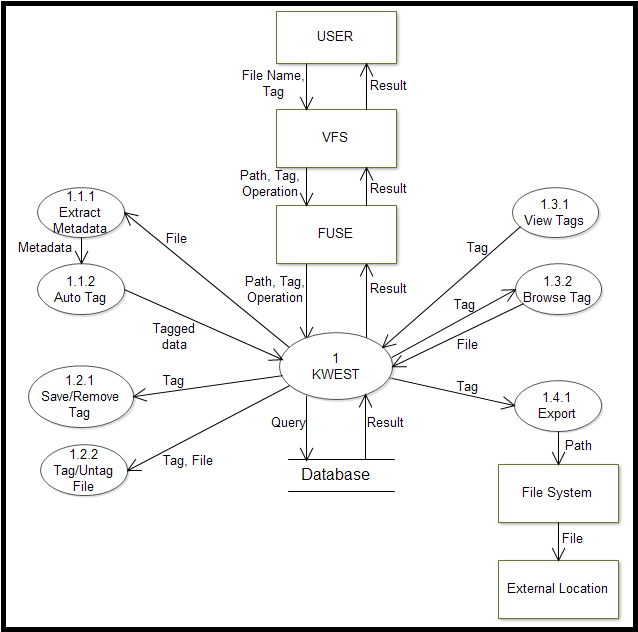
\includegraphics[width=0.9\linewidth]{./diagrams/dfd2.png}}
%\includegraphics[width=0.8\textwidth]{image.png}
\caption{Data flow diagram - Level 2}
\label{fig:dfd2}
\end{figure}

\newpage
\subsection {Entity Relationship diagram}
\begin{figure}[H]
\centering
\setlength\fboxsep{0pt}
\setlength\fboxrule{0.5pt}
\fbox{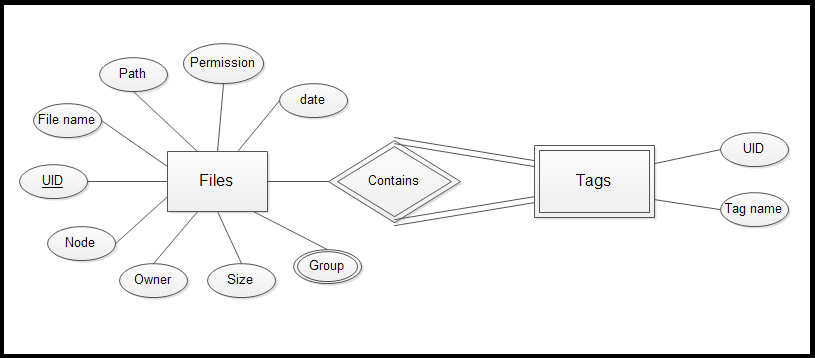
\includegraphics[width=0.8\linewidth]{./diagrams/ER.png}}
%\includegraphics[width=0.8\textwidth]{image.png}
\caption{Entity Relationship diagram}
\label{fig:ERdiag}
\end{figure}



\section{System Implementation Plan}

\subsection*{Phase 1: September 2012 - November 2012}
\begin{table}[h]
\begin{tabular}{|p{7cm}|p{2cm}|p{2cm}|}
\hline
\textbf {Task} & \textbf {Start Date} & \textbf{End Date} \\ \hline
Problem identification & 01/09/12 & 07/09/12 \\ \hline
Information gathering & 08/09/12 & 14/09/12 \\ \hline
Creating problem definition & 15/09/12 & 21/09/12 \\ \hline
Understanding underlying technology & 22/09/12 & 05/10/12 \\ \hline
Analyzing problem & 06/10/12 & 12/10/12 \\ \hline
Designing solution & 13/10/12 & 26/10/12 \\ \hline
Refining design & 27/10/12 & 02/11/12 \\ \hline
Creating design report & 03/11/12 & 09/11/12 \\
\hline
\end{tabular}
\caption{Phase 1 Implementation Plan}
\label{tab:P1plan}
\end{table}

\subsection*{Phase 2: December 2012 - March 2013} 
\begin{table}[h]
\begin{tabular}{|p{7cm}|p{2cm}|p{2cm}|}
\hline
\textbf {Task} & \textbf {Start Date} & \textbf{End Date} \\ \hline
Building a stub implementation & 01/12/12 & 14/12/12 \\ \hline
Implement file system operations & 15/12/12 & 28/12/12  \\ \hline
Extract Metadata from files & 28/12/12 & 11/01/13 \\ \hline
Implement modular plugins & 12/01/13 & 25/01/13 \\ \hline
Apply Apriori algorithm to database & 26/01/13 & 08/02/13 \\ \hline
Rigorous testing & 09/02/13 & 22/02/13  \\ \hline
Debugging and refining & 23/02/13 & 08/03/13 \\ \hline
System testing & 09/03/13 & 15/03/13  \\ \hline
Creating implementation report & 16/03/13 & 31/03/13 \\
\hline
\end{tabular}
\caption{Phase 2 Implementation Plan}
\label{tab:P2plan}
\end{table}
 %software requirment specification
%\input{sysdesign.tex} %system design
%\input{tech.tex} %technical specification
%\chapter{APPENDIX}
%\setcounter{section}{A}
\begingroup
\let\clearpage\relax
\phantomsection
\addcontentsline{toc}{section}{\protect\numberline{}\textbf{Appendix A:} Mathematical Model}%
\chapter*{A: MATHEMATICAL MODEL}
\endgroup
The relationship between files and tags can be represented by using Set theory. Set theory is the branch of mathematics that studies sets, which are collections of objects. The following mathematical model represents the working of this filesystem. 

\noindent The following dynamic and variable sets are defined as, \\
\indent $F$	: Set of Files \\
\indent $T$	: Set of Tags \\
\indent $S$	: Set of Tags in query ( $S \subseteq T$ ) \\

\subsection{Relation between Files (F) and Tags (T)}
$$ R = \{(f,t) \mid f \,\, has \,\, tag \,\,t; f \in F, t \in T\}$$
Here $R$ defines the relation between a file $f$ and its tag $t$ where $R \subseteq F \times T$. This relationship is \emph{many-to-many}. 
That is a file can have many tags, and a tag can describe many files.

\subsection{Association between Tags (T)}
Using discovered associations, we can form various relations between tags. These \emph{tag-to-tag} help in displaying related information. For any two tags there exists a distinct relation between them given by $r$. The function $X_{r}(A,B)$ returns the relation between two tags. Associations can be broadly categorized as:
\begin{itemize}
\item {$A \sim B$} : $A$ and $B$ are not directly related, but there \emph{may} exist some indirect relation between them.
\item $A \succ B$ : $A$ and $B$ are directly related, where $A$ always has a path leading to $B$. This relation is similar to $A \subset B$.
\item $A \bowtie B$ : $A$ and $B$ are not directly related, but $B$ supplements additional information related to $A$.
\item $\phi$ : This relation states that there does not exist any relation between the two tags.
\end{itemize}

\subsection{Operations}
$$g(f) = \{t : f \, R \, t\}$$
$g$ is an operation which takes input as a file $f$ and returns the set of tags ($t \in S$) related by $R$ to that file.

$$h(t) = \{f : f \, R \, t\}$$
$h$ is an operation which takes input as a tag $t$ and returns the set of files ($f \in F_{S}$) related by $R$ to that tag.

%----------------------------------------------------------------------------------------------------------------------------------

\subsection{Storing Tags and Files}
The relation $R$ is stored as a set of ordered pairs $(f,t)$, where $R \subseteq F \times T$. The operations $g$ and $h$ operate on these ordered pairs and return mapped or matched elements. A relation which has to be added must be represented in the form of of ordered pair $(f,t)$. Storage of all relations is given by $F \times T$ where ordered pairs exist according to $R = \{f \in F, t \in T \mid f\, R \,t\}$.

\noindent For example, we have the sets and their relations as: 
$$F = \{ f_{1}, f_{2}, f_{3} \}, T = \{ t_{1}, t_{2}, t_{3} \}, R = \{f_{1} \, R  \, t_{1}, f_{2}  \, R  \, t_{2}, f_{3}  \, R  \, t_{1}, f_{1}  \, R  \, t_{3}\}$$
Then we store this relation by its ordered pairs given by:
$$R = \{(f_{1},t_{1}),(f_{2}, t_{2}),(f_{3}, t_{1}),(f_{1}, t_{3})\}$$

\subsection{Extraction of metadata}
The extraction of metadata is defined by the function $X_{E}$ which takes a file $f(f \in F)$ and returns a set of tags $(T_{E} \subseteq T)$ that form the relation ($f  \, R  \, t : t \in T_{E}$). 
$$X_{E}(f) = T_{E} \in 2^{T}$$

\noindent Addition of new information (metadata, tags) is done as:
$${if (t \notin T) \, then \, (T \gets T \cup \{t\})}$$

\noindent We then store this relation as a ordered pair $\{(f, \, t) \, \forall t \in T_{E}\}$. At the end of this operation $T_{E} \subseteq T$ will hold true. 

\subsection{Importing Semantics}
The existing file-directory structure can be imported to the system and represented in the form of tags and files. We define: 

\noindent $F_{H} \, $  : Set of \emph{Files} on hard-disk which are not represented in system.\\
$D_{H}$ : Set of \emph{Directories} on hard-disk which are not represented in system. \\

\noindent Then for every file stored within a directory $d$, the relation $R$ is expressed as 
$(f  \, R  \, d)$.
When importing semantics we create the ordered pair $(f,d)$ given by the relation $(f  \, R \,  d, \forall d \in D_{d})$. Where $D_{d}$ contains the directory the file is stored in, as well as every parent directory of that directory itself.

\noindent Directories also contain sub-directories which we store in the form of tag relationships. We represent them as:
$\forall (d_{1}, d_{2}) \in D_{H}$, if $d_{2} \subset d_{1}$ ($d_{2}$ is a sub-directory of $d_{1}$) store the relation as
$$d_{1} \to d_{2}$$


\subsection{Apriori Algorithm}
The apriori algorithm\cite{FastAlgo} is a classic algorithm for learning association rules. The
 algorithm is designed to operate on databases containing transactions. As is
common in association rule mining, given a set of itemsets (for instance, sets
of retail transactions, each listing individual items purchased), the algorithm
attempts to find subsets which are common to at least a minimum number C of the
itemsets. Apriori uses a "bottom up" approach, where frequent subsets are
extended one item at a time (a step known as candidate generation), and groups
of candidates are tested against the data. The algorithm terminates when no
further successful extensions are found.

The purpose of the apriori algorithm is to find associations between different sets of data.
Each set of data has a number of items and is called a transaction.
The output of Apriori is sets of rules that tell us how often items are contained in sets of data.

\subsubsection{Itemset}
A collection of one or more items. \\
Example: {A, B, C} \\ \\
\textbf{k-itemset} \\
An itemset that contains k items.

\subsubsection{Support count (S)}
Number of transactions containing an itemset. \\
Example: S({A, B}) = 2

\subsubsection{Support (supp)}
The support supp(X) of an itemset X is defined as the proportion of transactions in the data set which contain the itemset.
Suppose \textit{minsup} is the minimum support threshold.
Example: supp({A, B}) = 2/5

\subsubsection{Frequent Itemset (L)}
An itemset satisfies minimum support if the occurrence frequency of the itemset
is greater or equal to a threshold. If an itemset satisfies minimum support, then it is a frequent itemset.
Thus an itemset whose support is greater or equal to minsup is a frequent itemset.

\subsubsection{Confidence}
The confidence of a rule is defined as,\\
\begin{equation}
Conf(A \rightarrow B) = supp(A \rightarrow  B) / supp(A)
\end{equation}
Suppose \textit{minconf} is the minimum confidence threshold.

\subsubsection{Rule Generation}
Given a set of transactions T, the goal of association rule mining is to find all rules having\\
\begin{equation}
support \geq minsup \; threshold
\end{equation}
\begin{equation}
confidence \geq minconf \; threshold
\end{equation}

Given a frequent itemset L, find all non-empty subsets $f \subset L$ such that $f \rightarrow  L - f$ satisfies the minimum confidence requirement.

Example: If ${A, B, C}$ is a frequent itemset, then the following candidate rules are formed \\
${ AB \rightarrow  C, \; AC \rightarrow  B, \; BC \rightarrow  A, \; A \rightarrow  BC, \; B \rightarrow  AC, \; C \rightarrow  AB }$ 

If $|L| = k$, then there are $(2 ^ k) - 2$ candidate association rules 
$(ignoring \,\; L \rightarrow \Phi \; and \;\; \Phi \rightarrow L)$

\subsubsection{Apriori principle}
The princciple sttes that if an itemset is frequent, then all of its subsets must also be frequent.
Apriori principle holds due to the following property of the support measure:
\begin{equation}
\forall X , Y : ( X \subseteq Y ) \rightarrow  s( X ) \geq s(Y )
\end{equation}

Support of an itemset never exceeds the support of its subsets. This is known as the anti-monotone property of support.

$\newline$
\textbf{Algorithm} \\
Input \\
T - Database of transactions \\
I   - Items \\
L - Itemset\\
s   - support\\
c - confidence

$\newline$
Output \\
R - Association rules satisfying s and c

$\newline$
Algorithm to Generate Frequent Itemsets\\
Apriori(T,s)\\
$L_{1} \leftarrow {Large \; 1-itemset} \\
k \leftarrow 2 \\
while \; L_{k - 1} \neq \Phi \\
C_{k} = Generate(L_{k - 1}) \\
	for \;  transactions  t \in T \\
		C_{t} \leftarrow Subset(C_{k}, t) \\
		for \; candidates \; c \in C_{t} \\
			count[c] \leftarrow \; count[c] + 1 \\
		L_{k} \leftarrow {c \in C_{k} | count[c] \geq s} \\
		k \leftarrow k + 1 \\
return \cup L_{k}$

$\newline$
Algorithm to Generate Association Rules\\
GenRule\\
$R = \Phi;\\
	for \; each \; l \in L \; do \\
		for \; each \; x \subset l \; such \; that \; x \neq \Phi \; and \; x \neq l \; do \\ 
			if (supp(l) \; / \; supp(x)) \geq c \; then \\
				R = R \; \cup \; ( x \rightarrow ( l - x ) )$;
				
				
				
\newpage				
\setcounter{subsection}{1}
\setcounter{subsubsection}{1}
\phantomsection
\addcontentsline{toc}{section}{\protect\numberline{}\textbf{Appendix B:} Testing of Data}
\chapter*{B: TESTING OF DATA}

Testing of the system will be done on the following points:

\subsection{Storing the relation $R$:}
The working of the system depends on correctly storing the relation $R$. These tests check whether the relations are stored and represented correctly. 
\begin{enumerate}
\item For any file $f$ associated with tag $t$ there should exist an ordered pair $(f,t)$.
\item For a file $f$ associated with tags $S = \{t_{1}, t_{2}, t_{3}\}$, the operation $g(f)$ should return exacty $S$.
\item For a tag $t$ containing files $F = \{f_{1}, f_{2}, f_{3}\}$, the operation $h(t)$ should return exactly $F$.
\end{enumerate}

\subsection{Relation between tags: }
\begin{enumerate}
\item The relation $r$ between two tags $t_{1},t_{2}$ is given by function $X_{r}(t_{1},t_{2})=c$.
\item The relation $r$ is distinct i.e. there exists only one relation between any two tags. If contradictions arise where more than one relation is present between two tags, then all those relations must be made void and $r=\phi$. The user can then explicitly specify which relation should be created between those two tags.
\item Extensive testing must be done on relations to determine which $r$ needs to be set under certain conditions.
\end{enumerate}

\subsection{Extraction of Metadata:}
Let $M$ be the set of all metadata tags $t$ for file $f$. The function $X_{E}$ represents an algorithm to extract t from f. It returns a set $T_{E}$ such that $\{t \in T_{E} \mid f \, R \, t\}$ and $(T_E \subseteq M)$. To test the efficiency of the function, or the effectiveness of it, we compare the cardinality of the generated set $T_E$ with the set of Metadata $M$. The efficiency can be calculated by
$$\mathrm{Efficiency} \, \epsilon = \frac {\mid T_E \mid} {\mid M \mid}$$
Using $\epsilon$ we can compare algorithms and their efficiency. Appropriate algorithms can be chosen for various file types so that efficiency of the entire system remains high. For e.g. \\
\indent $X_{E1} : \{\epsilon =0.7$ for audio$, \epsilon = 0.4$ for images $\}$ \\
\indent $X_{E2} : \{\epsilon =0.6$ for audio$, \epsilon = 0.6$ for images $\}$ \\
Then we have the following options:
\begin{enumerate}
\item $X_{E2}$ is a better choice as it yeilds a more consisten efficiency.
\item $X_{E1}$ is used only for audio and $X_{E2}$ is used only for image extractions.
\end{enumerate}


\subsection{Queries and their results:}
Queries are parsed into tokens of the form $(t_1, \sigma , t_2)$. We need to test whether $\sigma $ returns the correct results for the query. A Query $Q(S)$ is said to be successfully executed when the expected result are shown.  
\begin{itemize}
\item The Query $q(t)$ for a single tag $t$ should return a set of files $(f \in F_{S})$ through the operation $h(t)$. 
\item In a query if no operation is given, Intersubsection should be performed. 
\item For Query $Q(S)$ the operations should be performed from left to right unless precedence is specified by paranthesis. 
\end{itemize}

Example:
\noindent Let $t_{1}, t_{2}, t_{3}$ be tags having the following files: \\
\indent $t_{1}$ : $\{photo_{1},photo_{2},doc_{1}\}$  \\
\indent $t_{2}$ : $\{photo_{1},doc_{1}, ppt_{1}\}$  \\
\indent $t_{3}$ : $\{photo_{1},doc_{3}\}$ 
\begin{enumerate}
\item $q(t) = F_{S}$ where $f$ should follow the relation $(f \in F_S \mid f \, R \, T)$. 
For example, q$(t_{1})$ returns $F_S = \{photo_{1},photo_{2},doc_{1}\}$.
\item Consider a query containing tags $S = \{t_{1}, t_{2}\}$. 
It generates results by performing the operations $Q(S) = q(t_{1})\sigma q(t_{2})$
where $\sigma $ is an operator.
\begin{enumerate}
\item Putting $\sigma = \cup$ for Union in query $Q(S) = q(t_{1})\cup q(t_{2})$; the result should be $F_S = \{photo_1, photo_2, doc_1, ppt_1\}$. 	
\item Putting $\sigma = \cap$ for Intersubsection in query $Q(S) = q(t_{1})\cap q(t_{2})$; the result should be $F_S = \{photo_1, doc_1\}$.
\item Putting $\sigma = \setminus$ for Set Difference in query $Q(S) = q(t_{1})\setminus q(t_{2})$; the result should be $F_S = \{photo_2\}$, whereas the query $Q(S) = q(t_{2}) \setminus q(t_{1})$ will return the result as $F_S = \{ppt_1\}$.
\item Putting $\sigma = \ominus$ for Symmetric Difference in query $Q(S) = q(t_{1})\ominus q(t_{2})$; the result should be $F_S = \{photo_2, ppt_1\}$.
\end{enumerate}

\item Consider a query containing tags $S = \{t_{1}, t_{2}, t_{3}\}$.
It performs operations as : $Q(S) = q(t_{1})\sigma_{1} q(t_{2})\sigma_{2} q(t_{3})$
The default order for processing is from left to right unless precedence is specified through parenthesis.

\begin{enumerate}
\item For the query $Q(S) = q(t_{1}) q(t_{2}) q(t_{3})$ the result will be returned as files $\{photo_{1}\}$
\item For the query $Q(S) = q(t_{1}) \cup q(t_{2}) \cap q(t_{3})$ the result will be returned as files $\{photo_{1}, doc_{1}, doc_{3}\}$
\end{enumerate}
\end{enumerate}

After verifying that individual queries return correct results, we must check whether $Q(S)$ runs correctly as well. This is done by seperating the query into tokens, and calculating their results in turn. It must be verified that results are correct and have not been mis-intepreted through tokenization of the query.
%----------------------------------------------------------------------------------------------------------------------------------------

\subsection{Forming Associations}
Consider a database, D, consisting of 9 transactions.
Suppose minimum support count required is 2 (i.e. $minsup = 2 / 9 = 22\%$ ).
Let minimum confidence required is $minconf = 70\%$.
We have to first find out the frequent itemset using apriori algorithm.
Then, Association rules will be generated using minsup and minconf.

\begin{center}
\begin{tabular}{|l|l|}
\hline
\textbf {TagID} & \textbf {Files} \\ \hline
T100 & F1, F2, F5  \\ \hline
T101 & F1, F2, F5  \\ \hline
T102 & F2, F4  \\ \hline
T103 & F2, F3  \\ \hline
T104 & F1, F2, F4  \\ \hline
T105 & F1, F3  \\ \hline
T106 & F2, F3  \\ \hline
T107 & F1, F3  \\ \hline
T108 & F1, F2, F3, F5  \\ \hline
T109 & F1, F2, F3  \\ \hline
\end{tabular}
\end{center}

$\newline$
\textbf{Step 1: Generating initial Candidate Itemset} \\
In the first iteration of the algorithm, each item is a member of the set of candidate.

\begin{center}
\begin{tabular}{|l|l|}
\hline
\textbf {Itemset} & \textbf {Support count} \\ \hline
\{F1\} & 6  \\ \hline
\{F2\} & 7  \\ \hline
\{F3\} & 6  \\ \hline
\{F4\} & 2  \\ \hline
\{F5\} & 2  \\ \hline
\end{tabular}
\end{center}

$\newline$
\textbf{Step 2: Generating 1-itemset Frequent Pattern} \\
The set of frequent 1-itemsets, L1, consists of the candidate 1-itemsets satisfying minimum support.

\begin{center}
\begin{tabular}{|l|l|}
\hline
\textbf {Itemset} & \textbf {Support count} \\ \hline
\{F1\} & 6  \\ \hline
\{F2\} & 7  \\ \hline
\{F3\} & 6  \\ \hline
\{F4\} & 2  \\ \hline
\{F5\} & 2  \\ \hline
\end{tabular}
\end{center}

$\newline$
\textbf{Step 3: Generating 2-itemset Frequent Pattern} \\
To discover the set of frequent 2-itemsets, L2, the algorithm uses L1 Join L1 to generate a candidate set of 2-itemsets, C2.
Next, the transactions in D are scanned and the support count for each candidate itemset in C2 is accumulated.
The set of frequent 2-itemsets, L2, is then determined, consisting of those candidate 2-itemsets in C2 having minimum support.

\begin{center}
\begin{tabular}{|l|l|}
\hline
\textbf {Itemset} & \textbf {Support count} \\ \hline
\{F1, F2\} & 4  \\ \hline
\{F1, F3\} & 4  \\ \hline
\{F1, F5\} & 2  \\ \hline
\{F2, F3\} & 4  \\ \hline
\{F2, F4\} & 2  \\ \hline
\{F2, F5\} & 2  \\ \hline
\end{tabular}
\end{center}

$\newline$
\textbf{Step 4: Generating 3-itemset Frequent Pattern}\\
The generation of the set of candidate 3-itemsets, C3, involves use of the Apriori Property. First, we generate C3 using L2 join L2. \\
\begin{center}
C3 = \{\{F1, F2, F3\}, \{F1, F2, F5\}, \{F1, F3, F5\}, \\
\{F2, F3, F4\}, \{F2, F3, F5\}, \{F2, F4, F5\}\}.
\end{center}
Now we will apply Apriori property to determine which candidate itemsets are frequent.

The 2-item subsets of \{F1, F2, F3\} are \{F1, F2\}, \{F1, F3\} and \{F2, F3\}.
Since all 2-item subsets of \{F1, F2, F3\} are members of L2, We will keep \{F1, F2, F3\} in C3.

The 2-item subsets of \{F2, F3, F5\} are \{F2, F3\}, \{F2, F5\} and \{F3, F5\}.
But, \{F3, F5\} is not a member of L2 and hence it is violating Apriori Property.
Thus we will remove \{F2, F3, F5\} from C3.
Therefore,
\begin{center}
C3 = \{\{F1, F2, F3\}, \{F1, F2, F5\}\}.
\end{center}
Now, the transactions in D are scanned in order to determine L3, consisting
of those candidates 3-itemsets in C3 having minimum support.

\begin{center}
\begin{tabular}{|l|l|}
\hline
\textbf {Itemset} & \textbf {Support count} \\ \hline
\{F1, F2, F3\} & 2  \\ \hline
\{F1, F2, F5\} & 2  \\ \hline
\end{tabular}
\end{center}

$\newline$
\textbf{Step 5: Generating 4-itemset Frequent Pattern}\\
The algorithm uses L3 Join L3 to generate a candidate set of 4-itemsets, C4.
Although the join results in \{\{F1, F2, F3, F5\}\}, this itemset is removed since its subset \{\{F2, F3, F5\}\} is not frequent.
Thus, $ C4 = \Phi $ , and algorithm terminates, having found all of the frequent items.
This completes our apriori algorithm.

$\newline$
\textbf{Step 6: Generating Association Rules from Frequent Itemsets} \\
For each frequent itemset 'l', generate all nonempty subsets of l.
For every nonempty subset s of l, output the rule $ s \rightarrow  (l-s) $ if $ supp(l) \; / \; supp(s) \geq minconf $

We had L = \{\{F1\}, \{F2\}, \{F3\}, \{F4\}, \{F5\}, \{F1, F2\}, \{F1, F3\}, \{F1, F5\}, \{F2, F3\}, \{F2, F4\}, \{F2, F5\}, \{F1, F2, F3\}, \{F1, F2, F5\}\}.

Consider l = \{F1, F2, F5\}. Its all nonempty subsets are \{F1, F2\}, \{F1, F5\}, \{F2, F5\}, \{F1\}, \{F2\}, \{F5\}.

The association rules are shown below, each listed with its confidence.
\begin{enumerate}
\item $R1: F1, F2 \rightarrow F5 \\
Confidence = supp\{F1, F2, F5\} / supp\{F1, F2\} = 2 / 4 = 50 \% $ \\
R1 is Rejected.
\item $R2: F1, F5 \rightarrow F2$\\
$Confidence = supp\{F1, F2, F5\} / supp\{F1, F5\} = 2 / 2 = 100 \% $\\
R2 is Selected.
\item $R3: F2, F5 \rightarrow F1$\\
$Confidence = supp\{F1, F2, F5\} / supp\{F2, F5\} = 2 / 2 = 100 \% $\\
R3 is Selected.
\item $R4: F1 \rightarrow F2, F5$\\
$Confidence = supp\{F1, F2, F5\} / supp\{F1\} = 2 / 6 = 33 \% $\\
R4 is Rejected.
\item $R5: F2 \rightarrow F1, F5$\\
$Confidence = supp\{F1, F2, F5\} / supp\{F2\} = 2 / 7 = 29 \% $\\
R5 is Rejected.
\item $R6: F5 \rightarrow F1, F2$\\
$Confidence = supp\{F1, F2, F5\} / supp\{F5\} = 2 / 2 = 100 \% $\\
R6 is Selected.
\end{enumerate}

In this way, we have found the following three strong association rules.
\begin{enumerate}
\item $F1, F5 \rightarrow  F2$
\item $F2, F5 \rightarrow  F1$
\item $F5 \rightarrow  F1, F2$
\end{enumerate}

%\newpage
%\input{testingofdata.tex}
\newpage
%\setcounter{section}{A}
\setcounter{subsection}{1}
\setcounter{subsubsection}{1}
\phantomsection
\addcontentsline{toc}{section}{\protect\numberline{}\textbf{Appendix C:} Papers Published}
\chapter*{C: PAPERS PUBLISHED}

%\begin{table}[h]
\begin{center}
\begin{tabular}{p{1cm}p{12cm}}

\textbf{Sr.No.} & \textbf{Paper Name} \\ 

$[1]$ & A. Gogte, S. Gupta, H. Pandit, R. Sharma, \textit{Using association rule learning in a Semantic file system}, International Conference on Advanced Computer Sciences and Information Technology, Pune, Februrary 15, 2013, 
pp. 29-31. $[\textbf{Published}]$\\

$[2]$ & A. Gogte, S. Gupta, H. Pandit, R. Sharma, \textit{KWEST - A Semantically Tagged Virtual File System}, International Conference on Advanced Computer Engineering and Applications, Trivandrum, 2012. $[Accepted]$\\

\end{tabular}
%\caption{Paper Published}
\end{center}
%\label{tag:PP}
%\end{table}

\subsection*{1.}
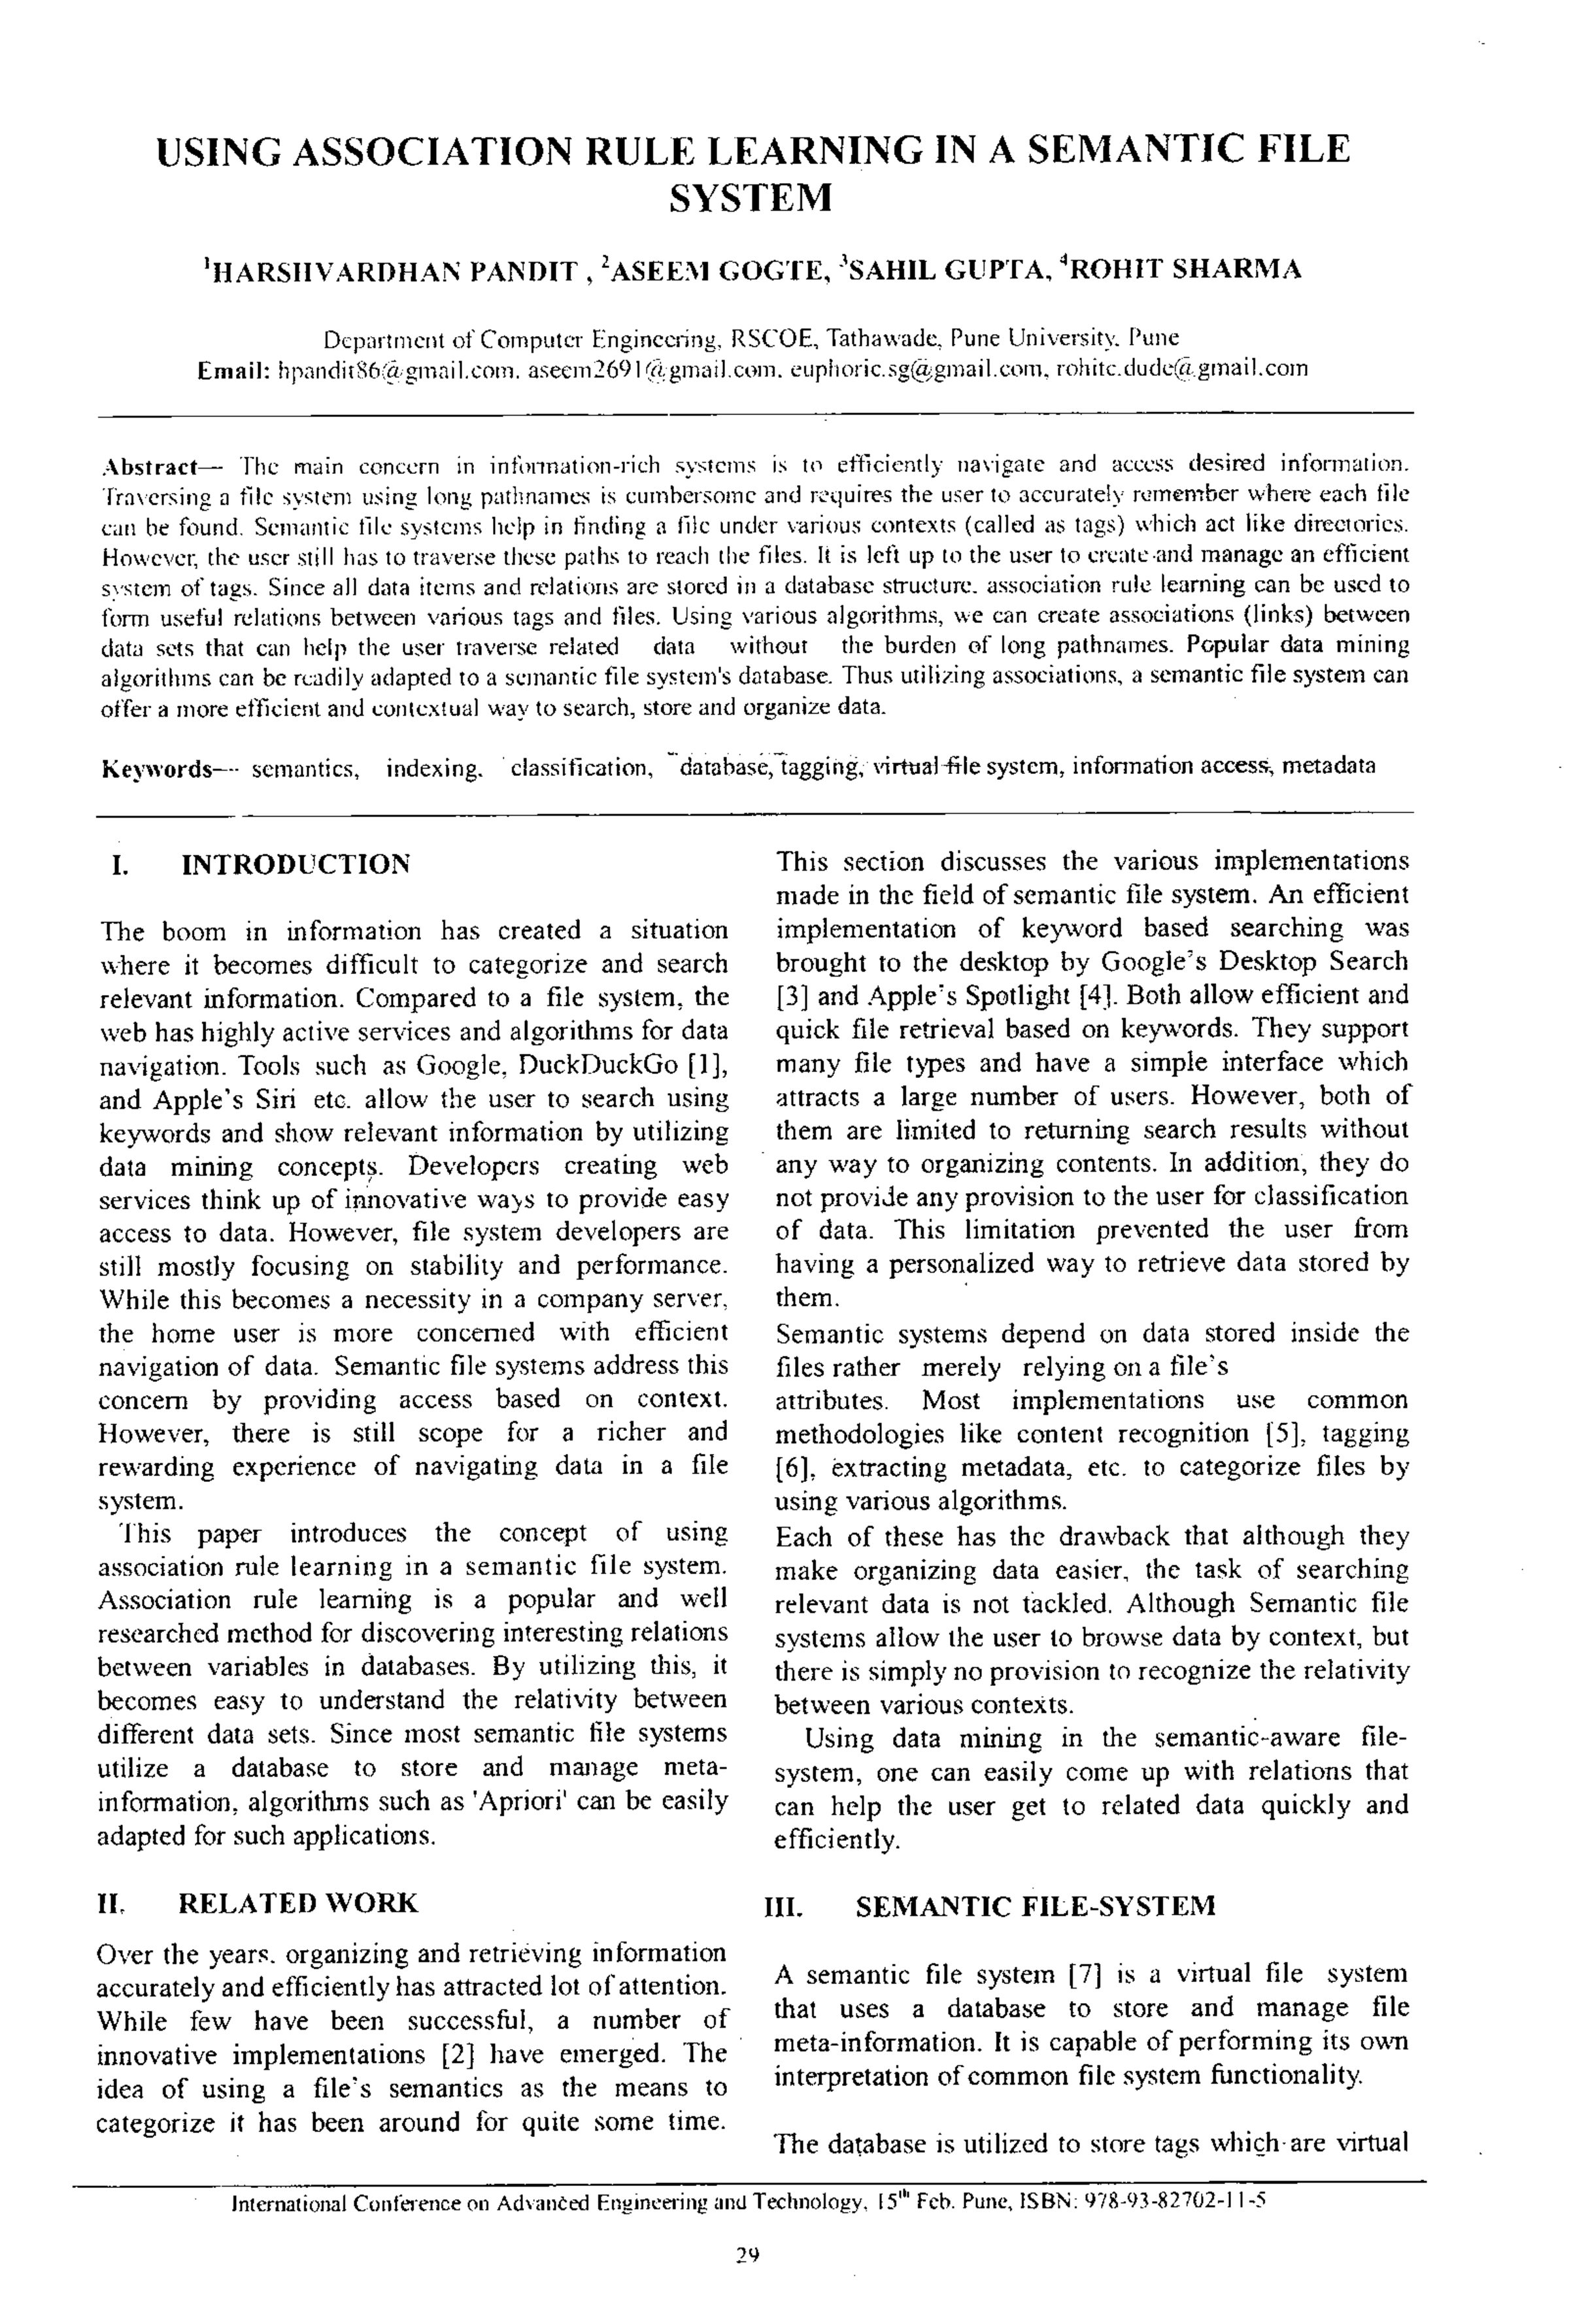
\includegraphics[page=1,scale=0.35]{./appendix/paperpage1.pdf}
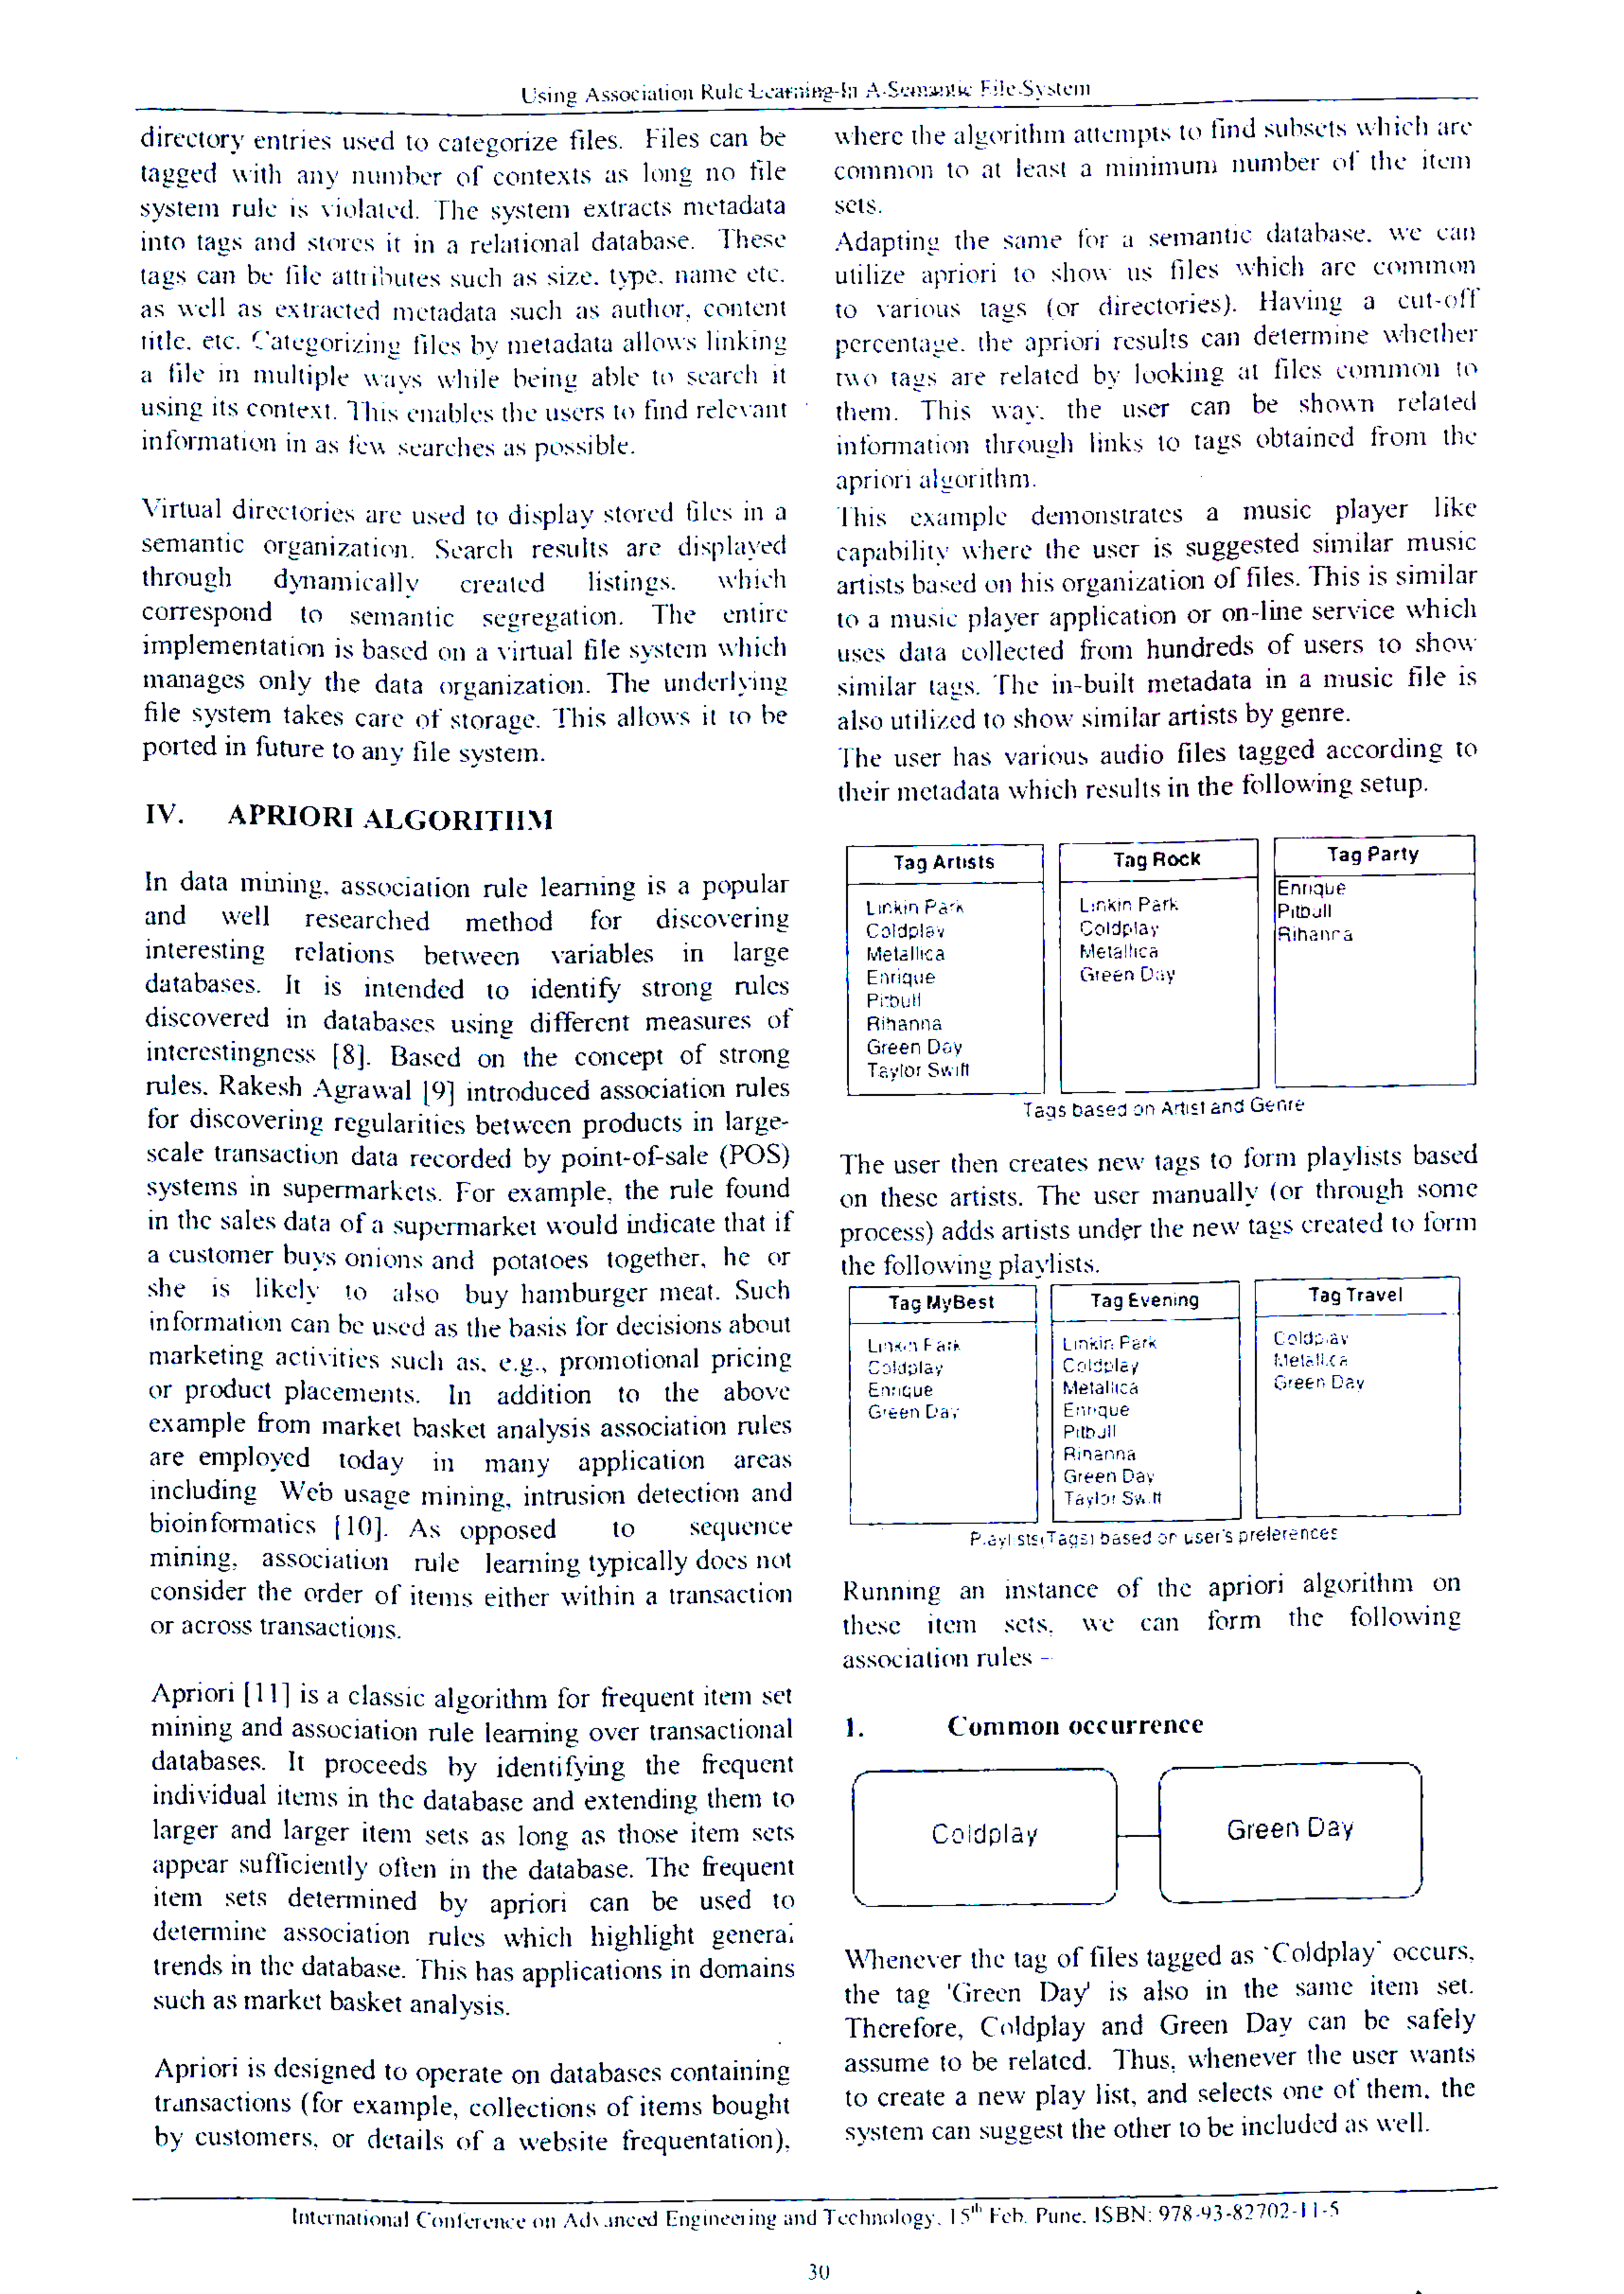
\includepdf[scale=0.85,pages=1-,offset=20 10,pagecommand={}]{./appendix/paperpage2.pdf}	
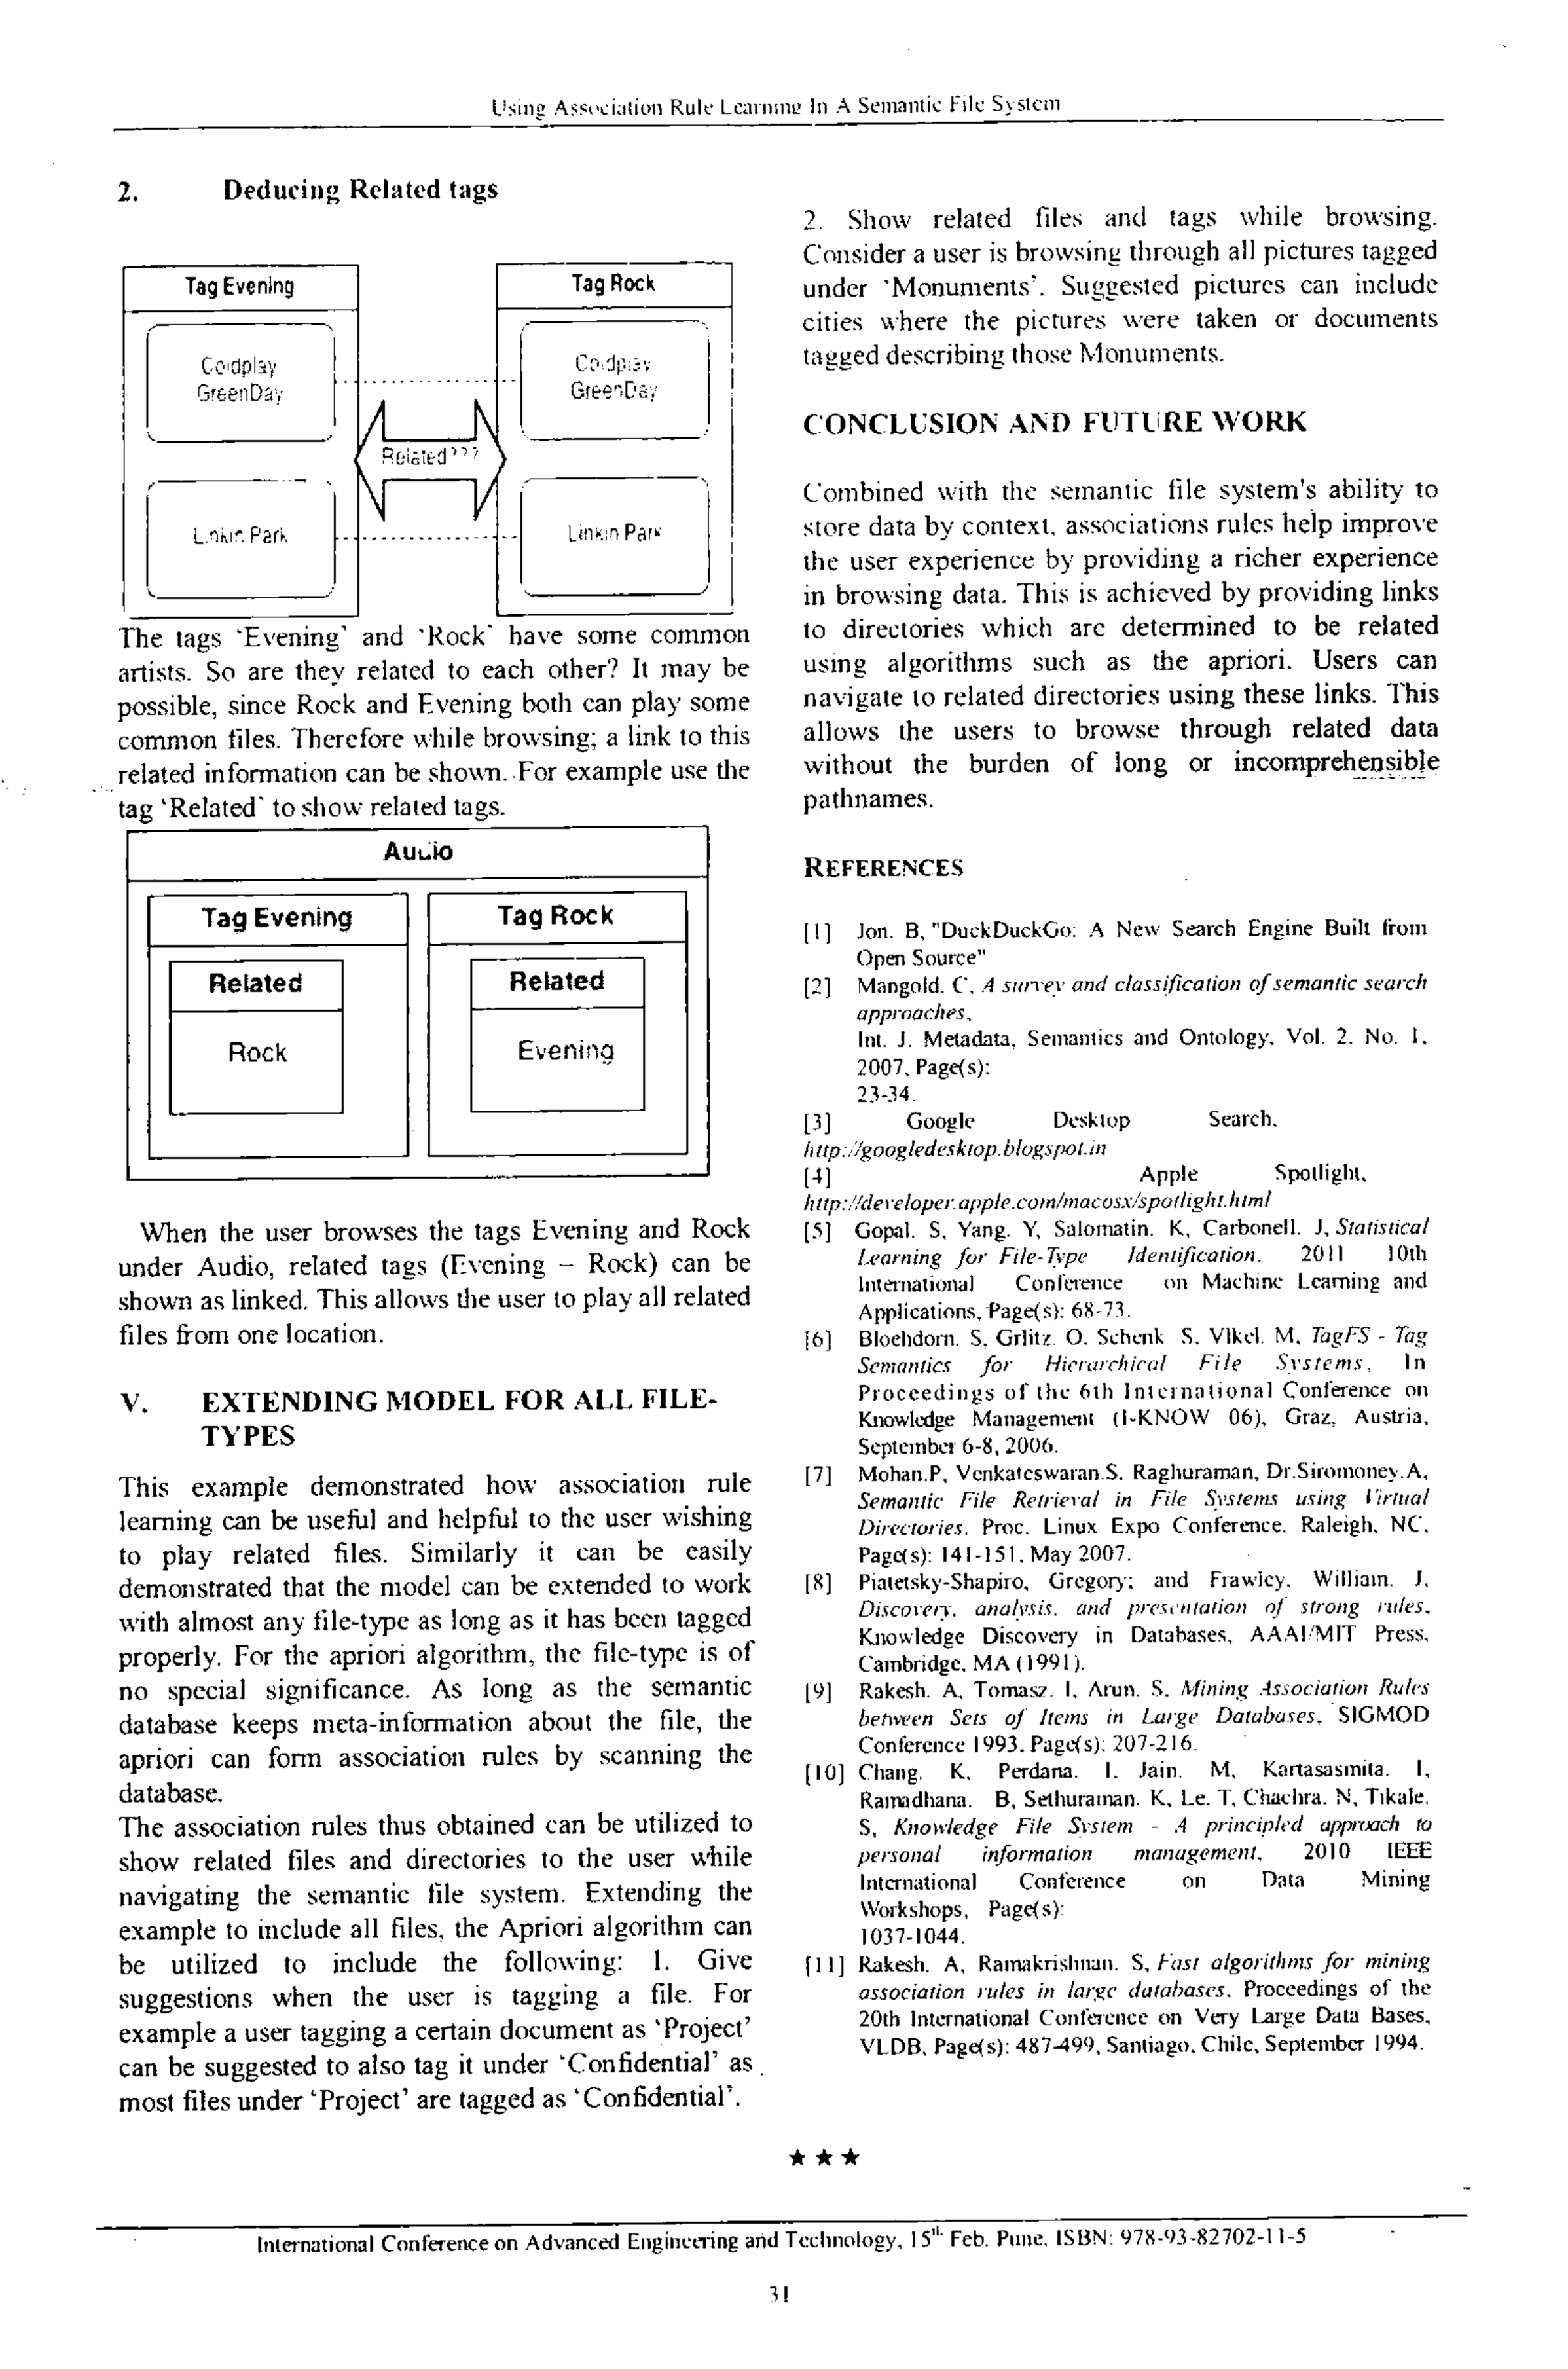
\includepdf[scale=0.85,pages=1-,offset=20 10,pagecommand={}]{./appendix/paperpage3.pdf}	

%\hspace*{-1.5cm}
\subsubsection{Reviewers comments:}
\begin{figure}[!h]
\centering
\setlength\fboxsep{0pt}
\setlength\fboxrule{0.5pt}
\fbox{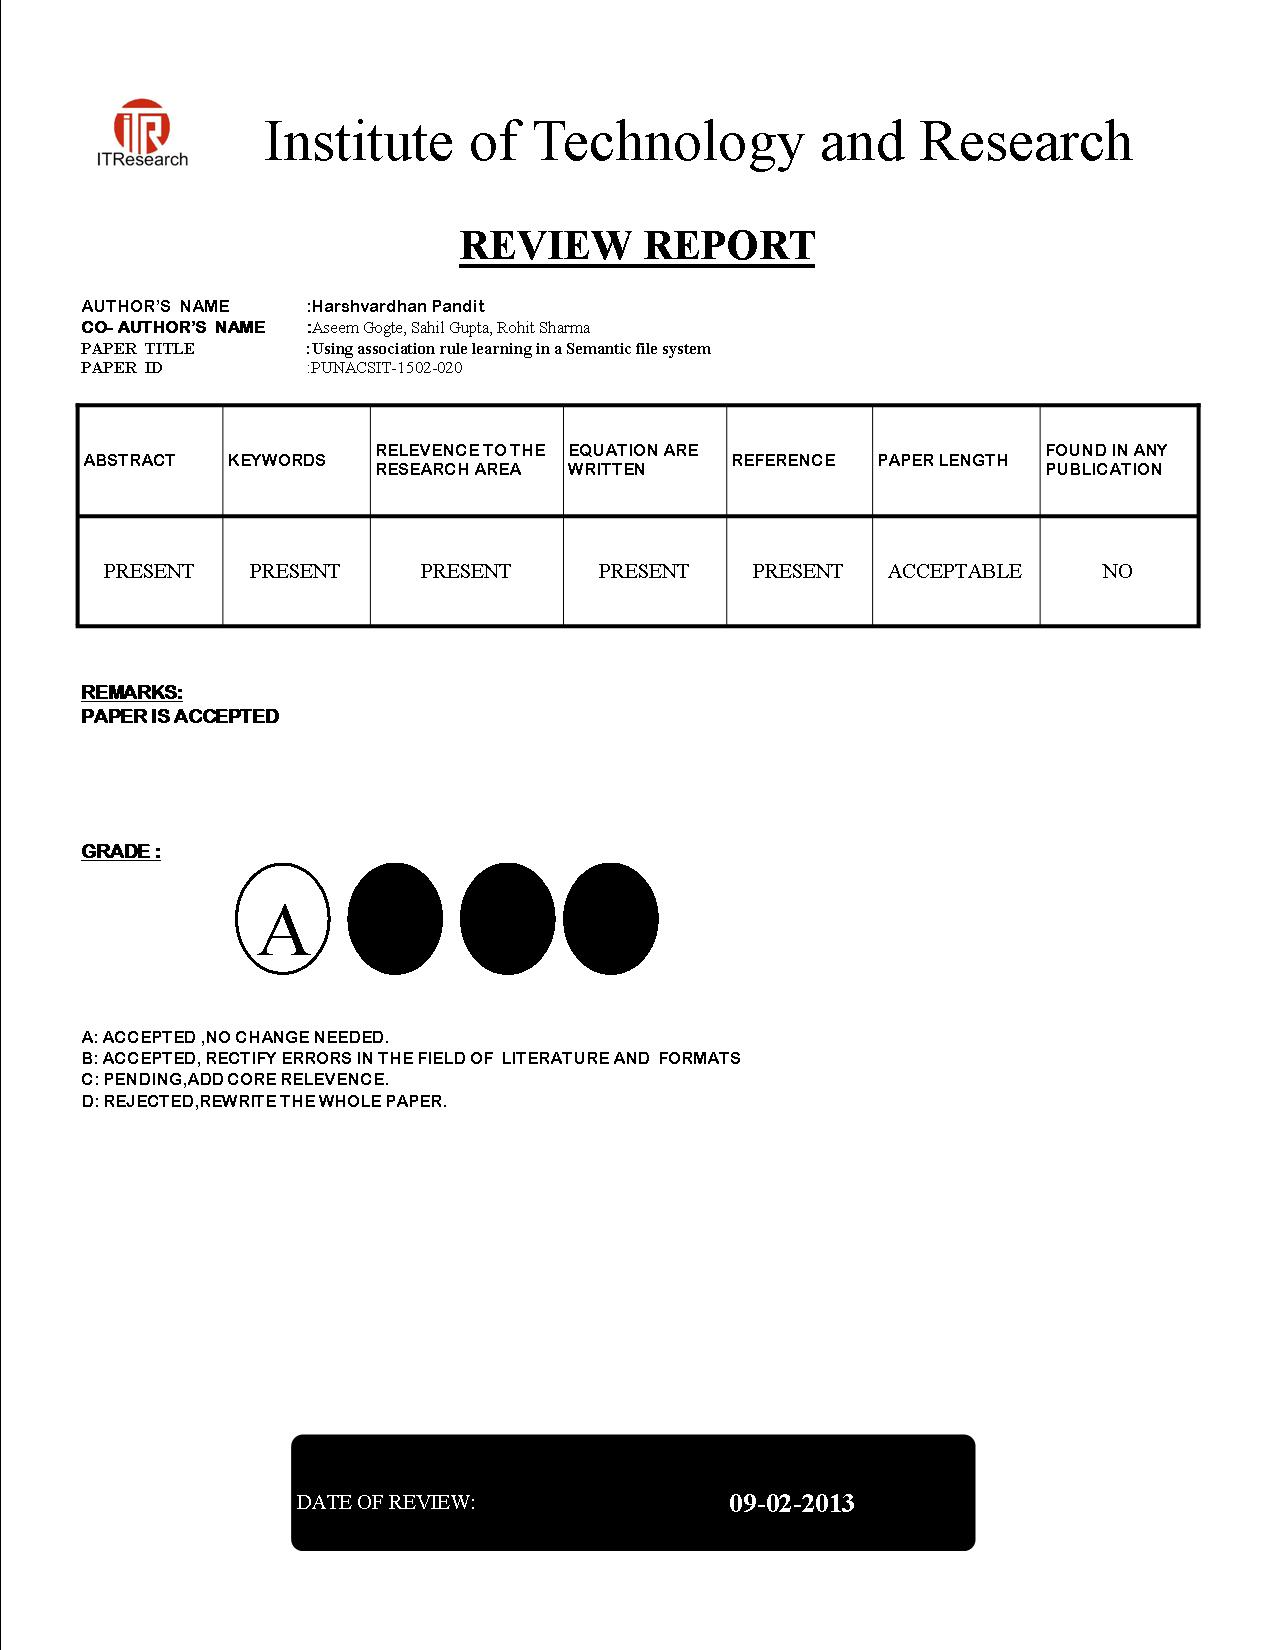
\includegraphics[width=0.8\linewidth]{./appendix/paper2review.jpg}}
%\includegraphics[width=0.8\textwidth]{image.png}
\caption{Reviewers comments}
\label{fig:RC1}
\end{figure}

\newpage
\subsection*{2.}

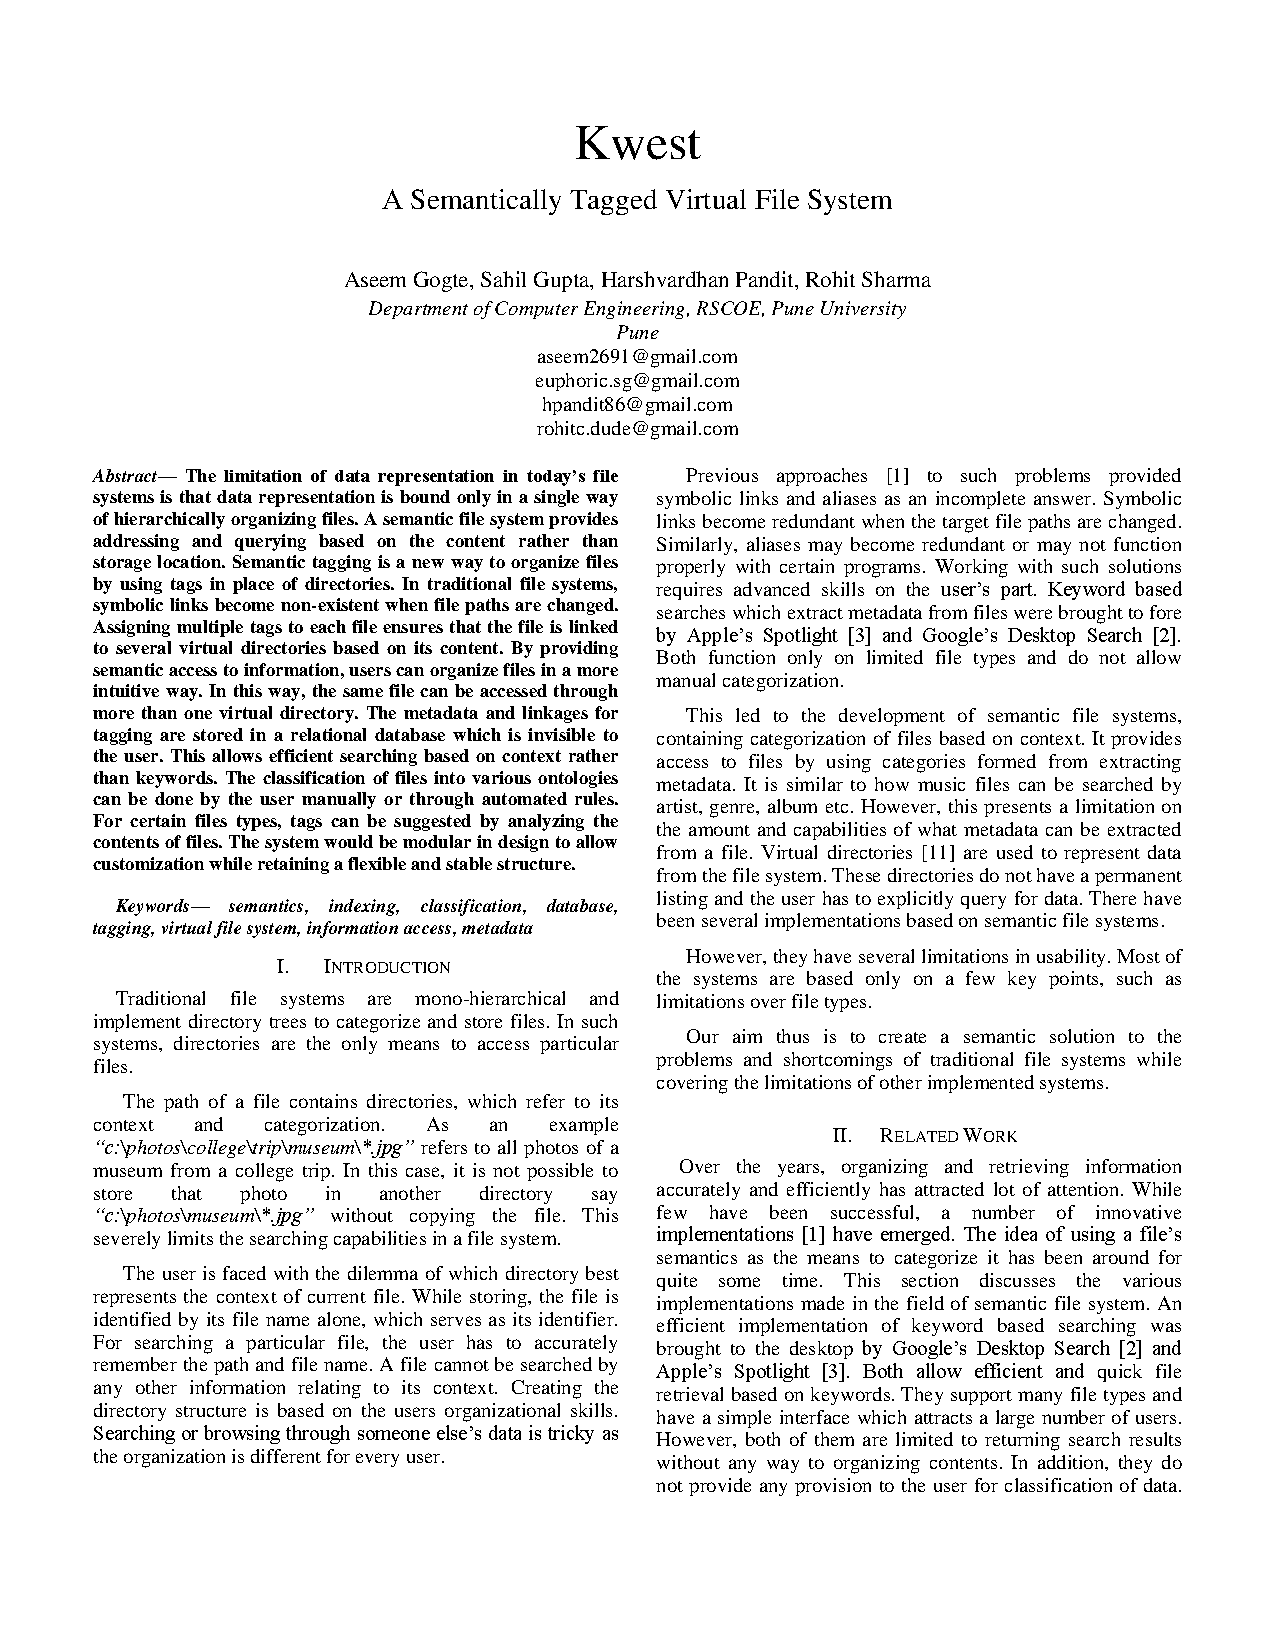
\includegraphics[page=1,scale=0.75]
{./appendix/sem1.pdf}
\includepdf[scale=0.85,pages=2-,offset=20 10,pagecommand={}]{./appendix/sem1.pdf}

\subsubsection{Reviewers comments:}
\begin{figure}[!h]
\centering
\setlength\fboxsep{0pt}
\setlength\fboxrule{0.5pt}
\fbox{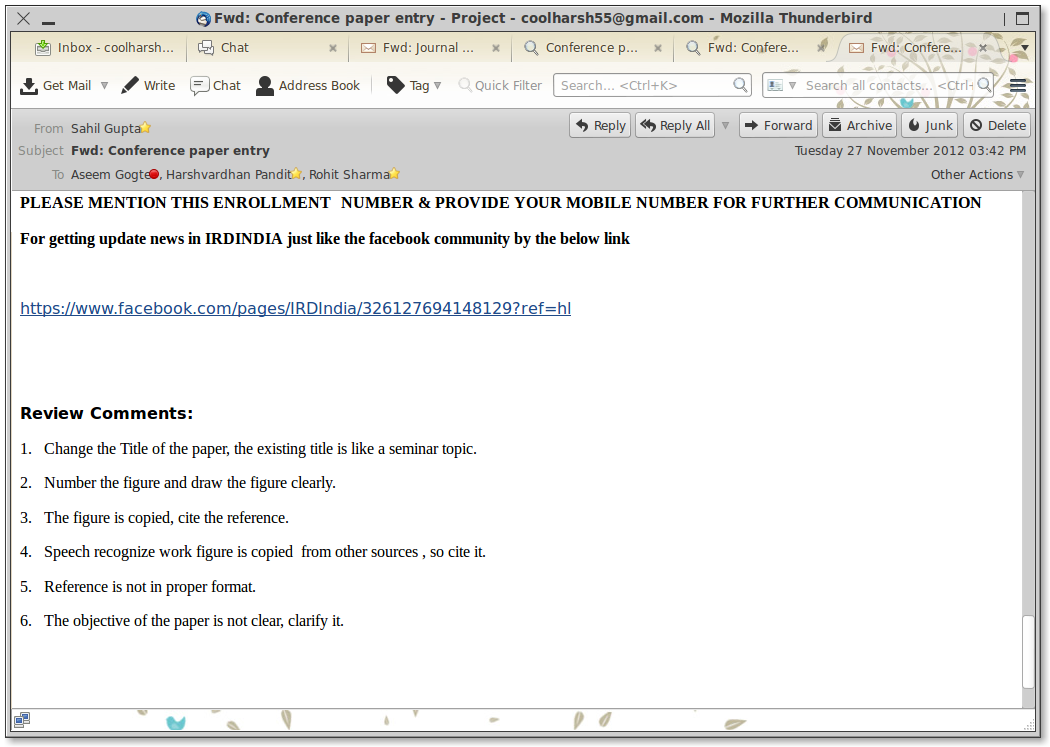
\includegraphics[width=0.8\linewidth]{./appendix/paper1review.png}}
%\includegraphics[width=0.8\textwidth]{image.png}
\caption{Reviewers comments}
\label{fig:RC2}
\end{figure}

\newpage
%\setcounter{section}{A}
\setcounter{subsection}{1}
\setcounter{subsubsection}{1}
\section*{APPENDIX D: PAPERS REFERRED}

\section{KFS - KNOWLEDGE FILE SYSTEM}
\hspace*{-1.5cm}
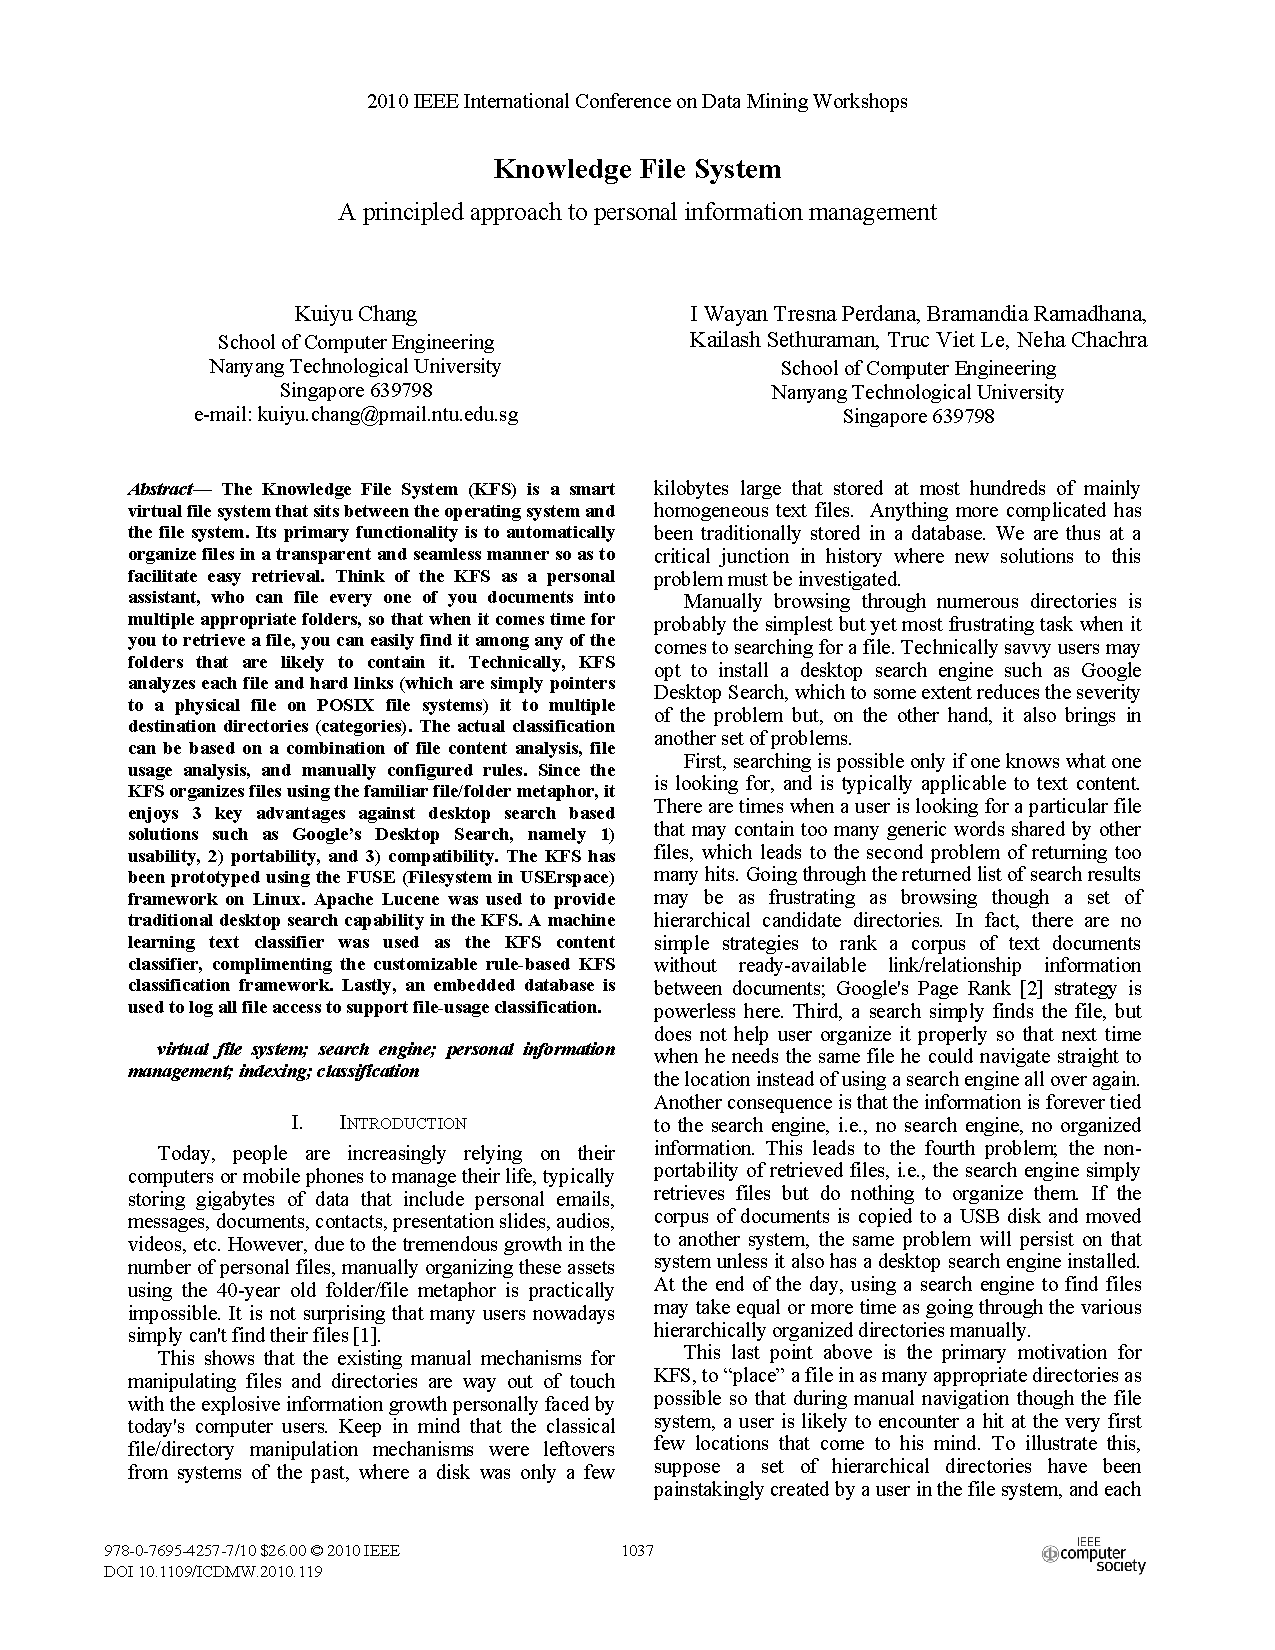
\includegraphics[page=1,scale=0.75]{./appendix/KFS.pdf}
\includepdf[scale=0.85,pages=2-,offset=20 10,pagecommand={}]{./appendix/KFS.pdf}


\section{Semantic-Aware Metadata Organization Paradigm in Next-Generation File Systems}
\hspace*{-1.5cm}
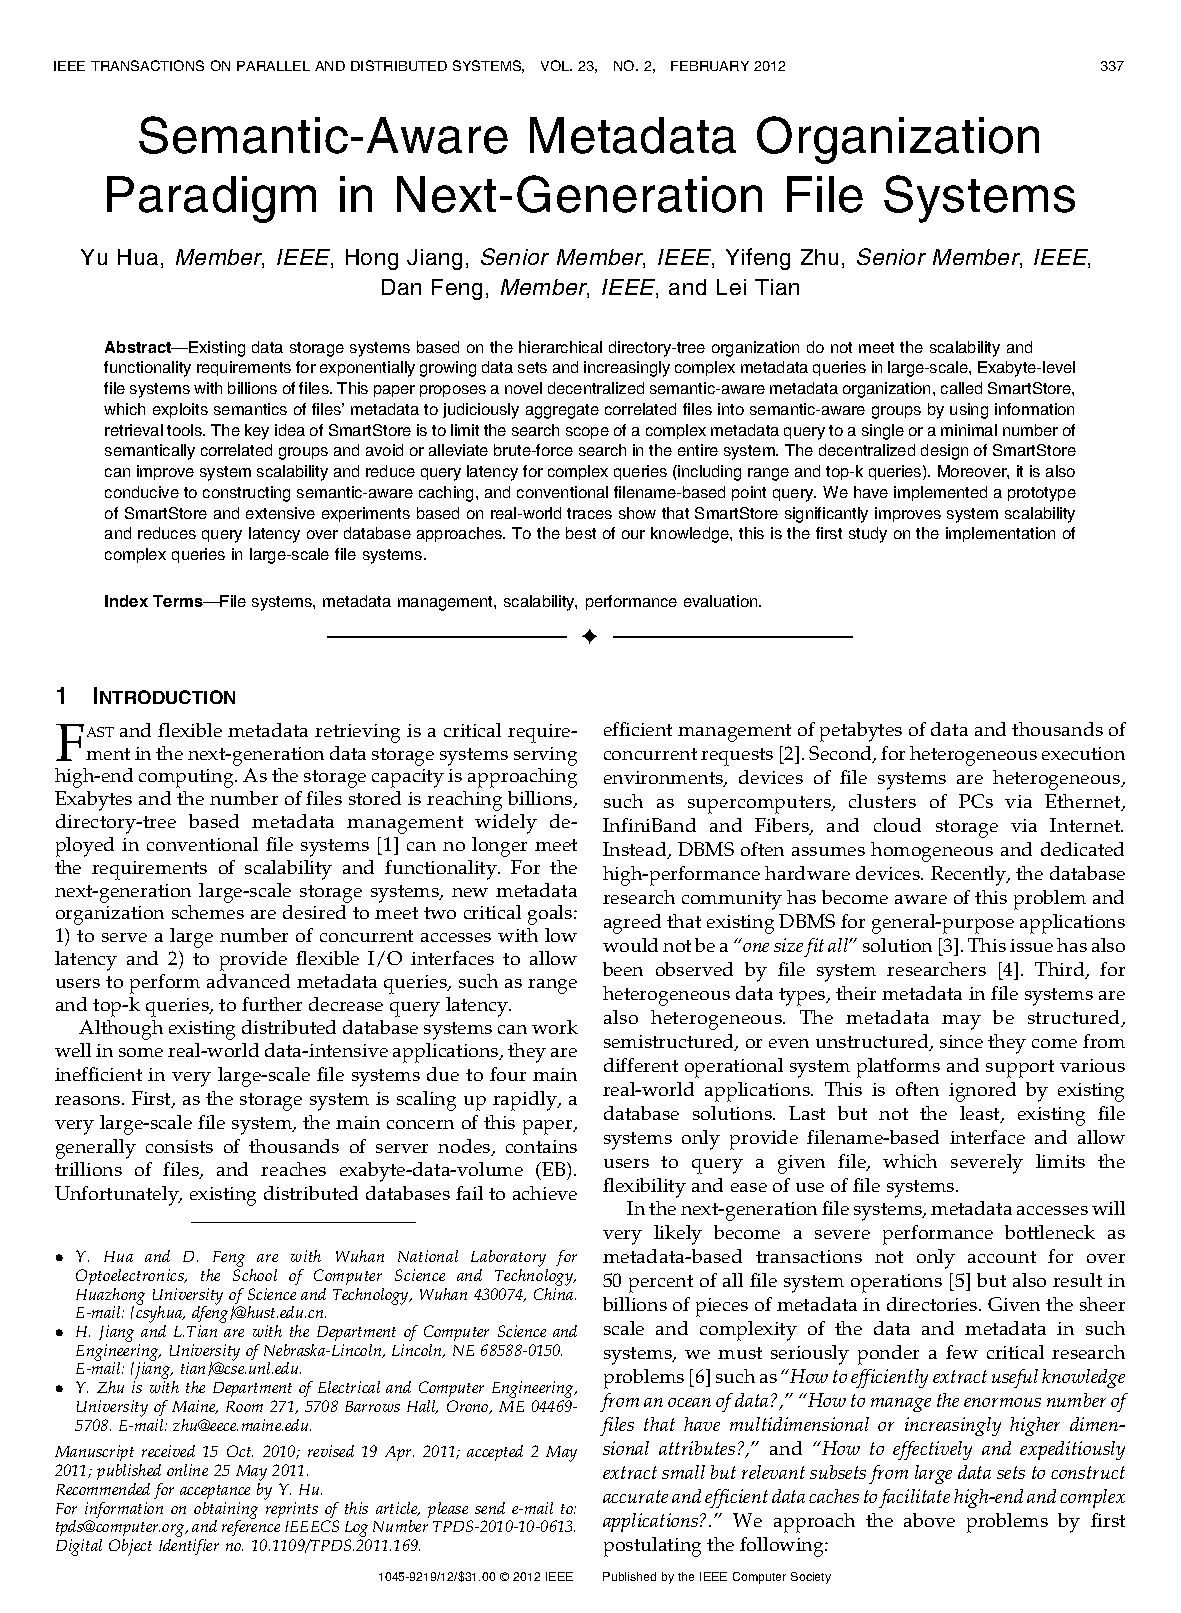
\includegraphics[page=1,scale=0.75]{./appendix/SM2012.pdf}
\includepdf[scale=0.85,pages=2-,offset=20 10,pagecommand={}]{./appendix/SM2012.pdf}	

\section{SEMANTIC FILE SYSTEM}
\hspace*{-1.5cm}
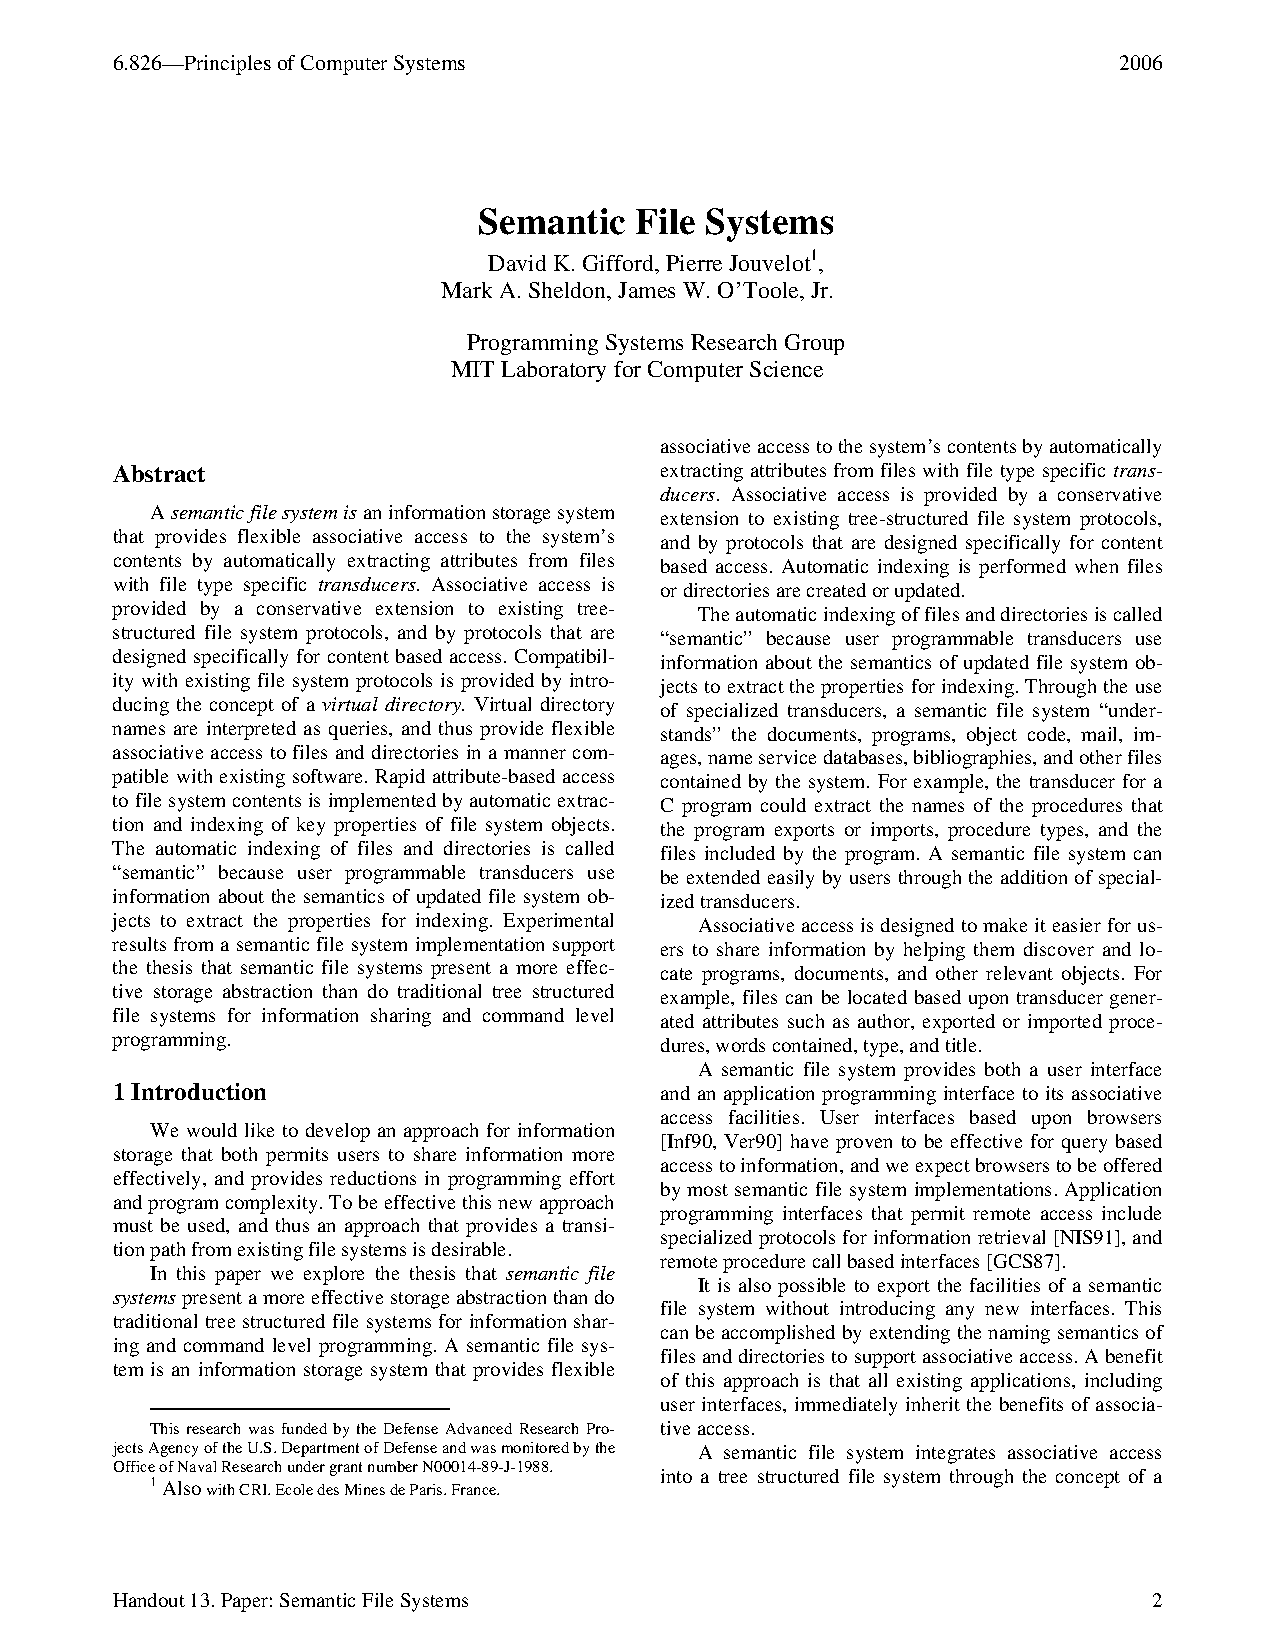
\includegraphics[page=1,scale=0.75]{./appendix/SEMFS.pdf}
\includepdf[scale=0.85,pages=2-,offset=20 10,pagecommand={}]{./appendix/SEMFS.pdf}



\newpage
%\setcounter{section}{0}
\setcounter{subsection}{1}
\setcounter{subsubsection}{1}
\section*{APPENDIX E : CONTRIBUTION OF TEAM MEMBERS} 
\emph{THIS SECTION IS A STUB. IS YET TO BE IMPLEMENTED...}
\noindent \textbf{Member 1: Aseem Gogte} 
\begin{itemize}
\item Mathematical Model
\item Testing related to Database 
\item Extraction of Metadata from Images \\
\end{itemize}

\noindent \textbf{Member 2: Sahil Gupta}
\begin{itemize}
\item Tag relations and behavior
\item Designing database queries
\item Database Design \\
\end{itemize}

\noindent \textbf {Member 3: Harshvardhan Pandit} 
\begin{itemize}
\item Interact with FUSE technology
\item Design Program flow
\item Component design \\
\end{itemize}

\noindent \textbf {Member 4: Rohit Sharma} 
\begin{itemize}
\item Extraction of Metadata from Audio / Video 
\item Database Design
\item Testing related to File operations
\end{itemize}



\newpage
%\setcounter{section}{0}
\setcounter{subsection}{1}
\setcounter{subsubsection}{1}
\chapter*{APPENDIX F: GLOSSARY}

\noindent \textbf{Acronyms} 
\begin{enumerate}
\item FUSE - File system in Userspace
\item GCC  - GNU Compiler Collection
\item GPL  - General Public License
\item API  - Application programming interface
\item GUI  - Graphical user interface
\item FAQ  - Frequently asked questions 
\item SFS  - Semantic File System
\item VFS  - Virtual File System
\item KFS  - Knowledge File System
\\
\end{enumerate}


\noindent \textbf{Term Definitions} \\
\begin{enumerate}
\item Semantic File System \\
Semantic File Systems are file systems used for information persistence which structure the data according to their semantics and intent, rather than the location as with current file systems. It allows the data to be addressed by their content (associative access) and querying for the data.
\item User Space \\
User space is that portion of system memory in which user processes run. This contrasts with kernel space, which is that portion of memory in which the kernel executes and provides its services.
\item File System \\
A 
file system 
is a 
means to 
organise 
data 
expected to be retained after a program 
terminates by providing procedures to store, retrieve and update data as well as 
manage the available space on the device(s) which contain it. 
\item Virtual File system \\
A virtual file system is an abstraction layer on top of a more concrete file system.
\item Virtual Directory \\
A virtual directory is a directory created in IIS to host our applications and to hide the actual physical location from the application users. 
It may simply designate a folder which appears in a path but which is not actually a sub-folder of the preceding folder in the path. 
\item Meta data \\
Metadata describes how and when and by whom a particular set of data was collected, and how the data is formatted.
\item Symbolic Links and Aliases \\
A symbolic link (also symlink or soft link) is a special type of file that contains a reference to another file or directory in the form of an absolute or relative path. 

%NEW NEW NEW NEW NEW NEW NEW NEW NEW NEW

\end{enumerate}




 %appendices

\chapter{Introduction}
\section{Overview}

Information organisation \cite{FUSE} and management is an essential and inevitable part of everyday computer usage. Huge amount of data is produced on daily basis \cite{GOOGLEDESKTOP}. With data growing in size, we are faced with the problem of locating files. Traditional file systems impose a  hierarchical structure of storage on the user. Traditional file systems are mono-hierarchical and implement directory trees to categorise and store files. In such systems, directories are the only means to access particular files.

In such systems, directories are the only means to access particular files. The path of a file contains directories, which refer to its context and categorisation. As an example \textit{``c:$\backslash$photos$\backslash$collegetrip$\backslash$museum*.jpg''} refers to all photos of a museum from a college trip. In this case, it is not possible to store that photo in another directory say \textit{``c:$\backslash$ photos$\backslash$museum*.jpg''} without copying the file. This severely limits the searching capabilities in a file system. The user is faced with the dilemma of which directory best represents the context of current file. While storing the file is identified by its file name alone which serves as its identifier. For searching a particular file, the user has to accurately remember the path and file name.

A file cannot be searched by any other information relating to its context. Creating the directory structure is based on the users organisational skills. Searching or browsing through someone else data is tricky as the organisation is different for every user. Previous approaches to such problems provided symbolic links and aliases as an incomplete answer. Symbolic links become redundant when the target file paths are changed. Similarly, aliases may become redundant or may not function properly with certain programs. Working with such solutions requires advanced skills on the users part. Keyword based searches which extract metadata from files were brought to fore by Apple's Spotlight and Google's Desktop Search. Both function only on limited file types and do not allow manual categorisation. This led to the development of semantic file systems, containing categorisation of files based on context. It provides access to files by using categories formed from extracting metadata. It is similar to how music files can be searched by artist, genre, album etc. However, this presents a limitation on the amount and capabilities of what metadata can be extracted from a file. Virtual directories are used to represent data from the file system. These directories do not have a permanent listing and the user has to explicitly query for data. There have been several implementations based on semantic file systems.

However, they have several limitations in usability. Most of the projects are based only on a few key points, such as limitations over file types. This project thus is to create a semantic solution to the problems and shortcomings of traditional file systems while covering the limitations of other implemented projects.

\section{Brief Introduction}
Organising and retrieving information accurately and efficiently has attracted a lot of attention. While few have been successful, a number of innovative implementations have emerged. KWEST is a virtual file system capable of storing semantics with which it facilitates the finding of relevant information. Information is stored in tags, which are extracted from a files metadata. This information may be generated implicitly by the system or supplied explicitly by the user. Thus, the validity of information is based on the user's level of organising things.

The current system can extract metadata from a limited set of known file types. However, the modular architecture allows for plugins to be added which can add functionality for other file types. This allows for the project to be extended and modified according to the functionality required. The level of awareness generated by the system is based on the frequency of access and input provided by the user. The amount of relevance is determined by the tags generated and their associated files. This affects how the system categorises and searches files. Thus the actual outcome of the system which is the searching capabilities is totally dependent on these relationships. The current implementation is based on the Linux kernel. Future implementations can be extended to other platforms and devices. Furthermore, as the system is a virtual one, it needs only slight modifications to be ported to other file systems and operating systems.

\section{Problem Definition}
The goal of this project is to develop a semantic file system that extracts metadata from files and allows storage and searching based on its context. Such a system should overcome the drawbacks of traditional file systems while leveraging the limitations of other such similar implementations.
		
\section{Feasibility Study}
\subsection{Technical Feasibility}
The team have knowledge of C and Object Oriented concepts. The Project is being implemented using loadable kernel module known as FUSE. In the current versions of some Linux based OS this module is included in the kernel itself.
The query processing and programming will be done using SQLite. It is a relational database contained in a small C programming library. In contrast to other database management systems, SQLite is not a process that is accessed from the client application, but an integral part of it. This is also open source and is freely available.
Thus, the cost for developing KWEST will be minimal and hence will be feasible without the need for large capital.
\subsection{Schedule Feasibility}
\subsection{Economic Feasibility}
Cost of Software: We have used open-source technologies for building our system, thus there was no software cost incurred.

Cost of Hardware: No hardware was required to be purchased, thus no cost was incurred in building the system.
\section{Application Of A Software Engineering Approach}
We are using incremental model of Software Development Life Cycle. The Systems development life cycle (SDLC) is a process used by a systems analyst to develop an information system, training, and user (stakeholder) ownership. The SDLC aims to produce a high quality system that meets or exceeds customer expectations, reaches completion within time and cost estimates, works effectively and efficiently in the current and planned Information Technology infrastructure, and is inexpensive to maintain and cost-effective to enhance.The System Development Life Cycle framework provides a sequence of activities for system designers and developers to follow. It consists of a set of steps or phases in which each phase of the SDLC uses the results of the previous one.A Systems Development Life Cycle (SDLC) adheres to important phases that are essential for developers, such as planning, analysis, design, and implementation.
\subsection{Planning}
During this stage, business opportunities and problems are identified, and information technology solutions are discussed. Multiple alternative projects may be suggested and their feasibility analysed.$\newline$ $\newline$ Tasks proposed were

		 \begin{enumerate}
			\item Analysing need of user to access related data.
			\item Identifying drawbacks of existing file system.
			\item The development of a project goals- identifying relations between data, file system operations, metadata storage, accessing related data.
			\item The collection of project requirements.
			\item The development of a project schedule.
			\end{enumerate}
					 
					 
\subsection{System Analysis}
The goal of system analysis is to determine where the problem is in an attempt to fix the system.This step involves breaking down the system in different pieces to analyse the situation, analysing project goals, breaking down what needs to be created and attempting to engage users so that definite requirements can be defined.$\newline$ $\newline$ Tasks proposed were


\begin{enumerate}
\item Interface for implementing file system.
\item Analyse various database alternatives based on size and speed of operation.
\item Analysis of libraries to be used for metadata operations.
\item Generation of files and tags suggestions.
\item Analysing various methods to provide user with suggestions.
\end{enumerate}
\subsection{System Design}
In systems design the design functions and operations are described in detail, including screen layouts, business rules, process diagrams and other documentation. The output of this stage will describe the new system as a collection of modules or subsystems.$\newline$ $\newline$ Tasks proposed were


				 \begin{enumerate}
				 \item Separating system implementation into following modules.
				 \item		File System Operations.
					\item	Generating Tags.
					\item	Importing Semantics.
					\item	Exporting Semantics.
					\item	Database Consistency.
				 \end{enumerate}
\subsection{Coding}
In coding we do actual implementation of system design, produced running software.$\newline$ $\newline$ Tasks proposed were


		\begin{enumerate}
		\item Implementing modules of project using finalised programming language and libraries
		\item Having modularity in code to allow for reusable modules.
			\item		Documenting the code using standard tools.
				\item		Testing project using various software testing approaches.
		\end{enumerate}
						
\subsection{Testing }
Testing is the process of evaluating a system or application, to check whether the application meets all requirements of the client and to detect the errors.$\newline$ $\newline$ Tasks proposed were


				
				\begin{enumerate}
				\item Testing of executable code using robust testing tools.
					\item Performing Regression Testing.
						\item Usability Testing.
						\item GUI Testing.
						\item Stress Testing.
						\item Integrity Testing.
				\end{enumerate}
						
\subsection{ Deployment}
Deployment starts after the code is appropriately tested, approved for release, and sold or otherwise distributed into a production environment. This may involve installation, customisation (such as by setting parameters to the customer's values), testing, and possibly an extended period of evaluation.$\newline$ $\newline$ Tasks proposed were
				\begin{enumerate}
				\item The project will be deployed as a executable which will mount the KWEST file system.
						 \item Utilise available GUI tools in the form of file managers.
						\item Installation of utility should follow standard Linux OS procedures.
		
				\end{enumerate}
						
\chapter{Literature Survey}
Over the years, organising and retrieving information accurately and efficiently has attracted lot of attention. While few have been successful, a number of innovative implementations\cite{SEMSURVEY} have emerged. The idea of using a file's semantics as the means to categorise it has been around for quite some time. This section discusses the various
implementations made in the field of semantic file system.

An efficient implementation of keyword based searching was brought to the desktop by Google's Desktop Search\cite{GOOGLEDESKTOP} and Apple's Spotlight\cite{SPOTLIGHT}. Both allow efficient and
quick file retrieval based on keywords. They support many file types and have a simple interface which attracts a large number of users. However, both of them are limited to returning search results without any way to organising contents. In addition, they do not provide any provision to the user for classification of data. This limitation prevented the user from having a personalised way to retrieve data stored by them.

Semantic systems depend on data stored inside the files rather merely relying on an file's attributes. Most implementations use common methodologies like content recognition\cite{STAT2011}, tagging \cite{TAGFS}, extracting metadata, etc. to categorize files by using various algorithms.

``Semantic File System''\cite{SEMFS}, as developed by O'Toole and Gittord in 1992, provides
access to file contents and metadata by extracting the attributes using special modules
called ”transducers”. It was one of the very first attempts to classify files by semantics
using metadata. Its biggest drawback was the need for file type specific transducers
which were necessary to extract meta information and content from the file. Also, the
user does not have any say in what kind of category the file is classified under. This
drawback makes it an unattractive option to the general user. It was decided during
designing KWEST, that it is necessary to involve the end-user in the tagging process. This
allows each user to have their own personal way of classification and organisation of
files.

NHFS (Non Hierarchical File System)\cite{NHFS} was a project developed by Robert Freund
in July 2007. It allows the user to place any file into any number of directories. Likewise,
any directory can be placed into as many directories as required. NHFS therefore allows
one to create a non-hierarchical structure with poly-hierarchically connected files. This
allows for a powerful metaphor of finding a file in any of the category (directory) it could
be stored under. Therefore, we decided to retain this feature by using tags in place of
actual directories. Tags are associated with files and other tags as well. Thus, a tag may
be placed under multiple tags allowing a relationship to be defined between them. This
analogy is much more powerful than restricting files to actual directories. Using tags
prevents duplication and redundancy, making it an efficient implementation.

A more recent implementation is Tagsistant\cite{TAGSISTANT} , which is a semantic file system that
also attempts to organise files using tags. It interacts with the Linux kernel using the
FUSE module. Under Tagsistant, directories are considered to be equivalent to tags. As
a consequence, creating a directory is creating a tag and putting a file inside a directory
means tagging that file. After you have tagged your files, you can search all of them by
using queries. Queries are just paths where each element is either a directory or logical
operators. The entire system has a modular design and uses SQLite. However, it suffers
from some speed issues and the lack of SQL indexes. Major flaws of this design were
high consumption of inodes on real file systems and high computational time which was
required to fulfil each request. Most of the features of Tagsistant were decided to be
included in KWEST. These were modular design, SQLite repository, tagged structure, etc.
which enhance the semantics of a file system. However, care must be taken to prevent
the occurrence of similar drawbacks.

Another implementation called Tagster\cite{TAGSTER} , is a peer-to-peer tagging application for
organising desktop data. It is platform independent and is implemented in JAVA. Multiple
files and also directories can be tagged through its interface. The selected directories are
recursively examined and all files contained within them are tagged. The GUI for a Linux
system consists of three main areas.

\begin{enumerate}
 \item Tag view 
 
 It displays a list of tags.
  
\item Resource view 

 It lists resources that have the currently selected tags assigned.
\item User view

 It displays a list of users that have tagged the currently selected resource
with some selected tag. It also includes GUI support for Windows with some unresolved
issues. However, it lacks auto classification of data due to which several common tags
may be generated for each user increasing the database size.

 \end{enumerate} 
\newpage For the development of KWEST, we referred to the following papers in order to
form a guideline for our project.

1. Chang. K, Ramadhana. B, Sethuraman. K, Le. T, Chachra. N, Tikale. S, Perdana. I,
Jain. M, Kartasasmita. I, Knowledge File System - A principled approach to personal
information management. 2010 IEEE International Conference on Data Mining
Workshops, Page(s): 1037-1044.\cite{KFS}

Abstract: The Knowledge File System (KFS) is a smart virtual file system that
sits between the operating system and the file system. Its primary functionality is to
automatically organise files in a transparent and seamless manner so as to facilitate
easy retrieval. Think of the KFS as a personal assistant, who can file every one of you
documents into multiple appropriate folders, so that when it comes time for you to
retrieve a file, you can easily find it among any of the folders that are likely to contain
it. Technically, KFS analyses each file and hard links (which are simply pointers to a
physical file on POSIX file systems) it to multiple destination directories (categories).
The actual classification can be based on a combination of file content analysis, file usage
analysis, and manually configured rules. Since the KFS organises files using the familiar
file/folder metaphor, it enjoys 3 key advantages against desktop search based solutions
such as Google's desktop Search, namely 1) usability, 2) portability, and 3) compatibility.
The KFS has been prototyped using the FUSE (File system in USErspace) framework
on Linux. Apache Lucene was used to provide traditional desktop search capability
		in the KFS. A machine learning text classifier was used as the KFS content classifier,
		complimenting the customisable rule-based KFS classification framework. Lastly, an
		embedded database is used to log all file access to support file-usage classification.
		
Usefulness: This paper describes approach to personal information management
		through Knowledge File System. It is designed to help users organise information
		using Virtual File System to reduce the problem of manual information classification and
		retrieval. KFS provides functions so as to automatically classify the information based
		on the content similarity with respect to predefined ontologies or also give the option
		for manual classification of the information. The operations carried out on the KFS can
		also be monitored with the event logger feature. Searching of files can be carried out by
		keyword with the help of a text indexer. Furthermore the comparisons between Google
		desktop file system, beagle and KFS are given. Finally the details of the implementation
		of the KFS on the Linux platform using of FUSE are given.
		
		2. Eck. O, Schaefer. D, A semantic file system for integrated product data management.
		2011 Advanced Engineering Informatics, Page(s): 177-184.\cite{SMFS2011}
		
		Abstract: We initially discuss a number of disadvantages of current file management
		systems. In the body of the paper our main contribution is presented. That is, a formal
		mathematical model of a new semantic file system, SIL (Semantics Instead of Location),
		that allows engineers to access data based on semantic information rather than storage
		location is proposed. A major difference between our approach and previous related work
		is that we do not aim at yet another point solution and, instead, propose an approach that
		may be employed by next generation engineering data processing systems on a larger
		scale. In addition, a corresponding programming interface along with a graphical user
		interface used as a file browser is presented and the benefits of utilising the proposed
		semantic file system for product data management in the field of integrated design of
		mechatronic systems are discussed.
		
		Usefulness: This paper describes a formal mathematical model that allows engineers
		to access data based on semantics rather than actual storage location. The main goal of
		this file system is to search files based on content of data. The browsing of the system is
		done based on file's metadata and attributes. Logical operator such as AND, OR, NOT
		are used to filter the results. The classification allows multiple tags to be created for files.
		Furthermore API's are written to create views and for the automation of notification
		updates.
		
		3. Mohan. P, Venkateswaran. S, Raghuraman, Siromoney. A, Semantic File Retrieval
		in File Systems using Virtual Directories. Proc. Linux Expo Conference, Raleigh, NC,
		Page(s): 141-151, May 2007.\cite{VIRDIR}
		
		Abstract: Hard Disk capacity is no longer a problem. However, increasing disk capacity
		has brought with it a new problem, the problem of locating files. Retrieving a document
		from a myriad of files and directories is no easy task. Industry solutions are being created
		to address this short coming. We propose to create an extendable UNIX based File
		System which will integrate searching as a basic function of the file system. The File
		System will provide Virtual Directories which list the results of a query. The contents
		of the Virtual Directory are formed at run time. Although, the Virtual Directory is used
		mainly to facilitate the searching of file, it can also be used by plugins to interpret other
		queries.
		
		Usefulness: This paper describes the design of SemFS, which provides semantics
		based on the file's meta-data and attributes. It allows the usage of logical operators to
		filter query results. It is implemented as a user space file system upon journaling storage.
		The architecture is server-client with support for API's to extend functionality. Features
		such as file tagging and versioning are also implemented.
		
		4.Rakesh. A, Tomasz. I, Arun. S, Mining Association Rules between Sets of Items in Large Databases, SIGMOD Conference 1993, Page(s): 207-216.\cite{MiningAssoc}
		
		Abstract :-We are given a large database of customer transactions. Each transaction consists of items purchased by a customer in a visit. We present an efficient algorithm that generates all significant association rules between items in the database. The algorithm incorporates buffer management and novel estimation and pruning techniques. We also present results of applying this algorithm to sales data obtained from a large retailing company, which shows the effectiveness of the algorithm.
		
		Usefulness :-For finding frequently occurring file and tags ,Creating association rules based on them give and providing suggestions to user.
		
		Many tagging systems exist that allow efficient manual classification of information.
		Most implementations tend to be theoretical\cite{SMO2012} demonstrations or complex
		implementations\cite{STMGMTSYS} existing for some very specific purpose. These suggest the
		possibility of using semantics\cite{SMFS2011} in operating systems in some future date. But a
		major problem is scalability with regard to related information. However, on a large
		multi-user file system, one can get tons of tags to shift through in each folder, increasing
		the load for users to search and maintain data. Our idea is to introduce a new concept
		of relating tags to overcome this situation. Implementing all the desired and necessary
		features from previous implementations, our design goal is to create an efficient Semantic
		File System which could be used by any class of users.
				

			

			



\chapter{Software Requirement Specification}
\section{Introduction}
\subsection{ Purpose}

[This presents comprehensive description of the intended purpose and environment of KWEST. It fully describes what the KWEST will do and how it will be expected to perform. In addition it also contains non-functional requirements.]

\subsection{ Intended Audience And Reading Suggestion}
The intended audience of this document includes both developers and reviewers of the system.

\subsection{Project Scope}
This project is a virtual file system capable of storing semantics with which it facilitates the finding of relevant information.
\begin{enumerate}
\item  Information is stored in tags, which are extracted from a file's metadata. This
information may be generated implicitly by the system or supplied explicitly by the
user.
\item  The validity of information is based on the users level of organising things.
\item  The system is currently designed to extract metadata from a limited set of popular
file types for audio, video and images and PDF documents.
\item  The modular architecture allows for plugins to be added which can add additional
functionality, and recognition for more file types. This allows the project to be
extended and modified according to the functionality required.
\item  The level of awareness generated by the system is based on the frequency of access
and input provided by the user.
\item  The current implementation is based on the Linux kernel. Future implementations
can be extended to other platforms and devices.
\item  As the system is an virtual entity, it does not need extensive modifications to be
ported to other file systems and operating systems.

\end{enumerate}

\subsection{User Classes And Characteristics} 

The system can be used by three types of users:
\begin{enumerate}
\item General User 

Uses the system without any complex modifications in the system.
\item Advanced User 

Understands the system and creates rules and automation’s based on personal needs.
\item Developer 

Uses the API provided and develops modules that extend the system.
Only advanced users utilise the semantic nature of underlying file system to the fullest.
This does not create any blocks for the general user, who can also use Kwest satisfactorily.
Developers are a different group of users who can extend Kwest through modules. These
modules can modify or define additional behaviour for the system for specific file types.
\end{enumerate}

\subsection{Operating Environment}\begin{enumerate}
\item  Kwest requires FUSE \cite{FUSE} version 2.8.6 and above.

\item Kwest can run on any Linux installation which contains required versions of FUSE.
\item  Furthermore, since kernel version 2.6.14, FUSE has been merged into the
mainstream Linux kernel tree. As a result Kwest can run on any Linux distribution
created from Kernel version 2.6.14 or above.

\item Kwest is a virtual file system mounted to a folder or a loop device.
\item It is the responsibility of the user that mounting and unmounting of the system be
done with standard rules and precaution

\end{enumerate}

\subsection{Design And Implementation Constraints}

Implementation Constraints
\begin{enumerate}
\item Kwest uses FUSE to manage userspace file systems. Hence, access is limited to the
executing userspace for the program.
 \item Since the entire application is executed in userspace only, there cannot be interaction
with the kernel directly.
\item Although Kwest implements a virtual file system which is accessible to all entities,
we have implemented the system with command line as the primary interface. Other
file managers such as Nautilus can only browse but not tag files. This limitation can
be addressed with plugins or additional modules built for the specific file manager.
\item The SQLite database is an integral part of Kwest and is contained in a single file. It
is vital for the system that integrity of the database is maintained.
\end{enumerate}
Design Constraints

\begin{enumerate}

\item Currently, the auto-tagging feature has been limited to common and popular file
types such as audio (mp3, wav, etc.), images (jpeg, png, etc.) and video (mp4, avi,
etc.). This functionality can be extended with modules or through special tools
made specifically for this purpose.

\item The amount of information visible through common file system commands (e.g.
ls - list contents) is a limitation for Kwest. We cannot show tagging information
through these interfaces. Alternate methods for this can be implemented keeping
the end user in mind.
\end{enumerate}


\subsection{ Assumptions And Dependencies}

Assumptions
\begin{enumerate}
\item Users of this software are aware of how semantics are used to categorise
information.
\item Users can recognise or identify appropriate tags in relation to files.
\item It is assumed that the user is well versed in organisation information and uses Kwest
as a tool rather than an assistant.
\item The user has the required privileges / rights to run Kwest and all its operations.
\end{enumerate}
Dependencies

\begin{enumerate}
 \item Kwest uses several external libraries to extract metadata from popular formats for
audio, images etc. TagLib, EXIF etc. which are required at compilation time. These
enable the system to handle metadata extraction for popular file formats.


 \end{enumerate} 


\section{System Features}
\subsection {Tags}
\begin{enumerate}
\item Manual Tagging 

Manual tagging is the basis of semantics in Kwest. The user can assign any tag to the files in Kwest. These tags are then stored internally in a database. The user can create new tags or use tags already defined by the system. Total freedom is given to the user to organise data. Multiple tags can be assigned to the to a single thus allowing its access through multiple locations without duplication of data.
\item Automatic Tagging 

Kwest also features automatic tagging of files. The user can define certain rules under which files will be assigned tags. The system will implement those rules for all files satisfying the defined constraints. This would prevent repetitive tagging operations for the user. 
\item Importing tags 

Certain popular file formats such as mp3, jpeg etc have metadata embedded in them. Kwest supports such popular format and uses this metadata to automatically assign tags to the files. This feature enables the user to collectively classify and store the data under these tags.
\end{enumerate}

\subsection{Database}
\begin{enumerate}
\item Consistency 

Kwest uses an internal database to store and manage data. It is vital that the database always remains consistent. Kwest uses logging mechanisms to ensure that operations on the database always reach an endpoint. 
\item Access 

The database files used by Kwest are not locked down or access restricted. The Kwest API provides facilities that can be used to access the database. However, this feature is made available with the understanding that the integrity of the database will be maintained always.
\end{enumerate}

\subsection{Relation With Existing Data}
\begin{enumerate}
\item Importing semantics 

Users already have certain organisational structures in the way they store data in file systems. Kwest imports these semantics by converting the storage hierarchy to tag-based hierarchy. This allows the entire file system to be imported into Kwest along with the users previous organisation structure. 
\item Files are executable ready 

The files can be directly executed through the virtual file system without making any modification to the files like audio, video files can be played through the virtual system, images can viewed and documents can be opened and read.  
\end{enumerate}

\subsection{Exporting Semantics}
\begin{enumerate}
\item Export file system 

As the entire file system exists as a virtual entity, Kwest provides the export feature. Where the file system can be exported to another system where the data can be imported by another instance of Kwest. 
\item Export tagged files 

It is also possible for the user to export data under certain tags to an external location. The semantic organisation showed by tags is converted to actual directories and files are then copied to these directories. This way the user can export Kwest semantics and data to outside locations.
\end{enumerate}
	
\subsection{Modularity}
\begin{enumerate}
\item Modules As Plugins 

Kwest is an extendable system. It can use external modules to increase functionality or to modify existing operations. Support for using modules is built into Kwest right from the design stage. Additional extraction libraries can be included using the plugin module.
\item Support for developers 

Kwest provides support to developers by providing access to all internal features and database. The API layer allows developers to easily supplement internal operations with their modules.
\end{enumerate}

\section {External Interface Requirements}

\subsection {User Interfaces}
The user can use the system through the command line. The system mounts a virtual file system which the user can use to navigate through. If the file explorer/browser supports virtual file system, the user can use that to navigate through the files. 

\subsection {Hardware Interfaces}
No hardware interfaces used as the file system exists as a virtual entity.

\subsection {Software Interfaces}
\begin{itemize}
\item FUSE\cite{FUSE} \\
Kwest uses FUSE to run the file system code in user space without editing the kernel code.The FUSE module provides only a ``bridge'' to the actual kernel interfaces. Major file system operations are defined by FUSE and forwarded to Kwest for implementation.
\item SQLite\cite{SQLITE} \\
Kwest uses SQLite database to store data. In contrast to other database management systems, SQLite is not a separate process but an integral part of Kwest. Database is accessed and modified for most of the operations performed by Kwest.
\end{itemize}
\subsection {Communication Interfaces}
Kwest can be accessed like any other file system via Command line or file managers like Nautilus, Thunar etc.

\section {Nonfunctional Requirements}

\subsection {Performance Requirements}
\begin {itemize}
\item Response Time \\
The response time for any action on the file system or the database should be reasonable under normal operational circumstances. 
\item Capacity \\
Kwest can be used by any user with sufficient permissions to initialise the filesystem. Subsequent operations like read, write, modify etc. are restricted by user permissions similar to normal file systems.
\item Scalability \\
Kwest provides suggestions and includes automated tagging rules for Audio, Video and Images. It also allows manual tagging of files by the user. Various modules can be further added for recognising and categorising other file types.
\end{itemize}

\subsection {Safety Requirements}
\begin{itemize}
\item Power Failure \\
The system maintains a log file for database. It prevents data corruption by committing data that has been fully written to the log. This should prevent most, if not all, data corruption.
\item Data Loss \\
If any file is accessed which is mentioned in database but deleted from the system then it is removed from the database and appropriate message is displayed to user.
\item Access Rights \\
The system checks if the file tagged is available to user for access. It does not allow files to be included which cannot be access by the user.
\end{itemize}

\subsection {Security Requirements}
Kwest can be used only by a single user with sufficient rights to execute the software. No other user will have permissions to modify tags and files in the system.

\subsection {Software Quality Attributes}
\begin{itemize}
\item Availability \\
The System shall be available from mounting the file system until its unmounted.
\item Updatability \\
The system shall allow for addition or deletion of files under tags.
\item Reliability
\begin{itemize}
\item The system shall save new tags created by active user.
\item The system shall save the file path of an active user to database whenever new files are added to a tag.
\item The system shall maintain a log file which records every operation on database.
\item The system shall modify database whenever tags or files are deleted.
\item The system shall remove file entries from database whenever it is unable to access them.
\end{itemize}
\item Portability \\
The system is implemented on Linux. It is compatible with various other Linux distributions like Ubuntu, Fedora, Red Hat, etc.
\item Testability \\
New modules designed to be added to the system, to identify file types other than audio, video and images must be tested to check if they are compatible with input-output format of the system.
\item Usability \\
The system does not have a large learning curve as the user deals with commands common to all file systems. Documentation provided for the system will include user manuals, developer reference and common FAQ.
\end{itemize}

\section{Other Requirements}
\subsection{Legal Requirements}

All the libraries, programs used in this project are open sourced under GPL. SQLite is a
database which is free to use, distribute or modify. The FUSE kernel module is merged
with the Linux Kernel, which is open sourced and freely available under GPL. There
are no proprietary or closed source products, libraries or interfaces used in this program.
The project Kwest and its subsequent implementations will be open sourced under the
GPL upon completion.

%\newpage
\section {Analysis Model}
\subsection {Data Flow diagram}
\vspace*{1.5cm}
\hspace{6.5cm} \textbf{Level 0} \\


\begin{figure}[H]
\centering
\setlength\fboxsep{0pt}
\setlength\fboxrule{0.5pt}
\fbox{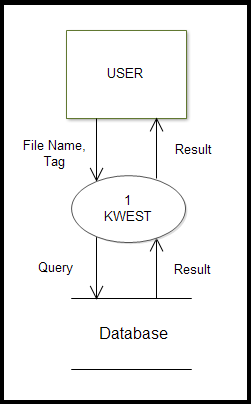
\includegraphics[width=0.5\linewidth]{./diagrams/dfd0.png}}
%\includegraphics[width=0.8\textwidth]{image.png}
\caption{Data flow diagram - Level 0}
\label{fig:dfd0}
\end{figure}

\newpage
\vspace*{2cm}
\hspace{5.5cm} \textbf{Level 1} \\
\begin{figure}[H]
\centering
\setlength\fboxsep{0pt}
\setlength\fboxrule{0.5pt}
\fbox{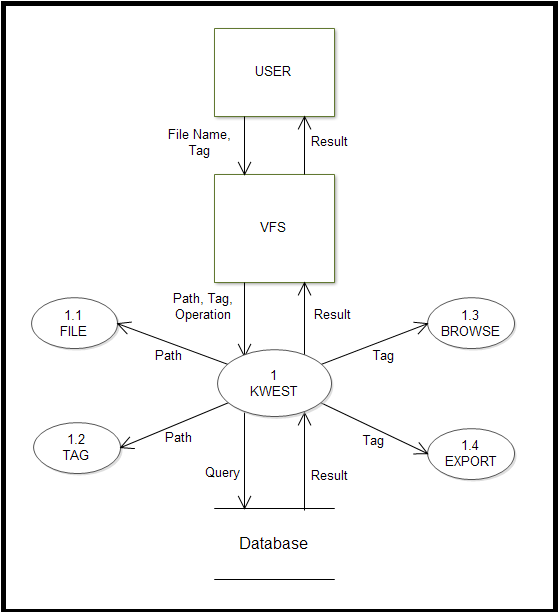
\includegraphics[width=0.9\linewidth]{./diagrams/dfd1.png}}
%\includegraphics[width=0.8\textwidth]{image.png}
\caption{Data flow diagram - Level 1}
\label{fig:dfd1}
\end{figure}

\newpage
\vspace*{2cm}
\hspace{5.5cm} \textbf{Level 2} \\
\begin{figure}[H]
\centering
\setlength\fboxsep{0pt}
\setlength\fboxrule{0.5pt}
\fbox{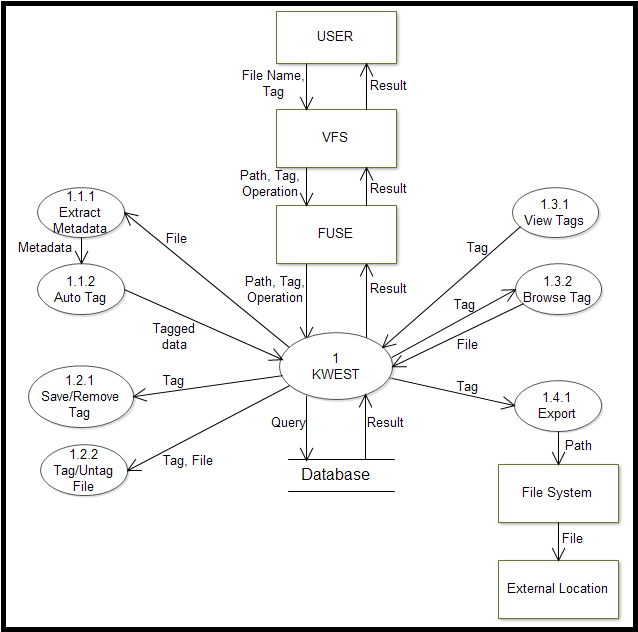
\includegraphics[width=0.9\linewidth]{./diagrams/dfd2.png}}
%\includegraphics[width=0.8\textwidth]{image.png}
\caption{Data flow diagram - Level 2}
\label{fig:dfd2}
\end{figure}

\newpage
\subsection {Entity Relationship diagram}
\begin{figure}[H]
\centering
\setlength\fboxsep{0pt}
\setlength\fboxrule{0.5pt}
\fbox{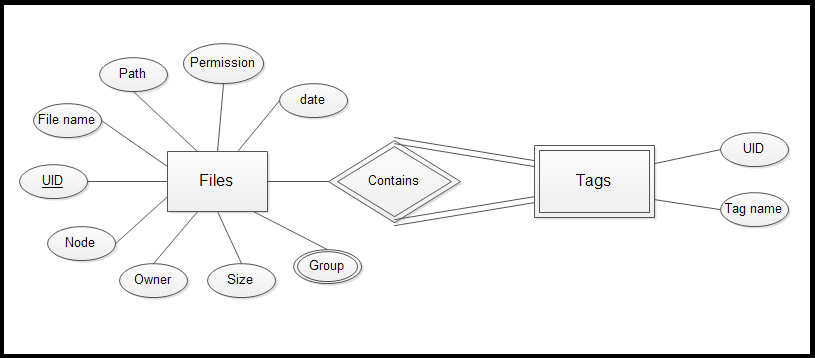
\includegraphics[width=0.8\linewidth]{./diagrams/ER.png}}
%\includegraphics[width=0.8\textwidth]{image.png}
\caption{Entity Relationship diagram}
\label{fig:ERdiag}
\end{figure}



\section{System Implementation Plan}

\subsection*{Phase 1: September 2012 - November 2012}
\begin{table}[h]
\begin{tabular}{|p{7cm}|p{2cm}|p{2cm}|}
\hline
\textbf {Task} & \textbf {Start Date} & \textbf{End Date} \\ \hline
Problem identification & 01/09/12 & 07/09/12 \\ \hline
Information gathering & 08/09/12 & 14/09/12 \\ \hline
Creating problem definition & 15/09/12 & 21/09/12 \\ \hline
Understanding underlying technology & 22/09/12 & 05/10/12 \\ \hline
Analyzing problem & 06/10/12 & 12/10/12 \\ \hline
Designing solution & 13/10/12 & 26/10/12 \\ \hline
Refining design & 27/10/12 & 02/11/12 \\ \hline
Creating design report & 03/11/12 & 09/11/12 \\
\hline
\end{tabular}
\caption{Phase 1 Implementation Plan}
\label{tab:P1plan}
\end{table}

\subsection*{Phase 2: December 2012 - March 2013} 
\begin{table}[h]
\begin{tabular}{|p{7cm}|p{2cm}|p{2cm}|}
\hline
\textbf {Task} & \textbf {Start Date} & \textbf{End Date} \\ \hline
Building a stub implementation & 01/12/12 & 14/12/12 \\ \hline
Implement file system operations & 15/12/12 & 28/12/12  \\ \hline
Extract Metadata from files & 28/12/12 & 11/01/13 \\ \hline
Implement modular plugins & 12/01/13 & 25/01/13 \\ \hline
Apply Apriori algorithm to database & 26/01/13 & 08/02/13 \\ \hline
Rigorous testing & 09/02/13 & 22/02/13  \\ \hline
Debugging and refining & 23/02/13 & 08/03/13 \\ \hline
System testing & 09/03/13 & 15/03/13  \\ \hline
Creating implementation report & 16/03/13 & 31/03/13 \\
\hline
\end{tabular}
\caption{Phase 2 Implementation Plan}
\label{tab:P2plan}
\end{table}

\chapter{SYSTEM DESIGN}
\section {System Architecture}
\begin{figure}[htb]
\centering
\setlength\fboxsep{0pt}
\setlength\fboxrule{0.5pt}
\fbox{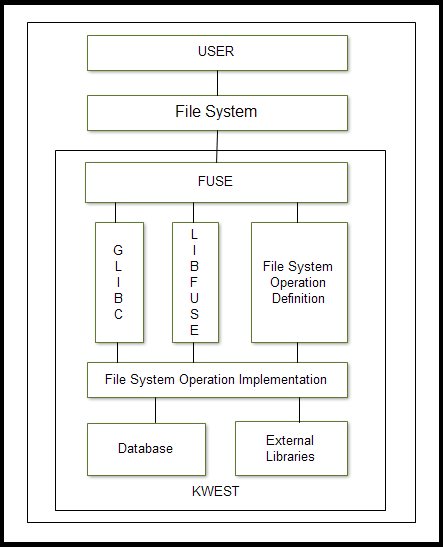
\includegraphics[scale=1.0]{./diagrams/sysarch.png}}
%\includegraphics[width=0.8\textwidth]{image.png}
\caption{System Architecture}
\label{fig:sys_arch}
\end{figure}

\newpage
\section {UML Diagrams}

\subsection {Use-case diagram}
\begin{figure}[htb]
\centering
\setlength\fboxsep{0pt}
\setlength\fboxrule{0.5pt}
\fbox{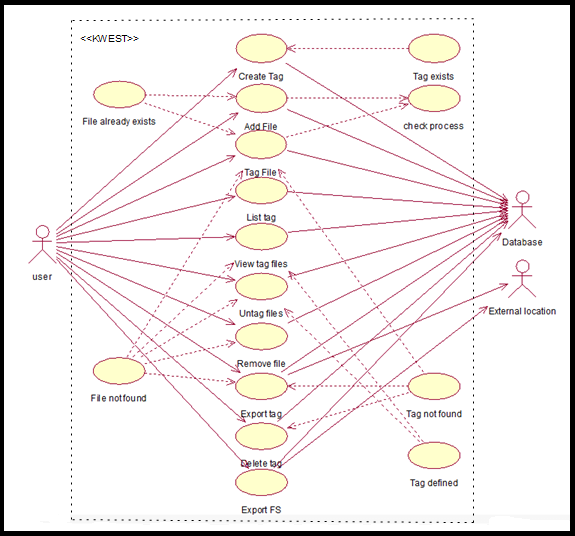
\includegraphics[width=1.0\textwidth]{./diagrams/usecase.png}}
%\includegraphics[width=0.8\textwidth]{image.png}
\caption{Use Case diagram}
\label{fig:usecase}
\end{figure}

%\subsection {Communication diagram}
%\begin{figure}[htb]
%\centering
%\setlength\fboxsep{0pt}
%\setlength\fboxrule{0.5pt}
%\fbox{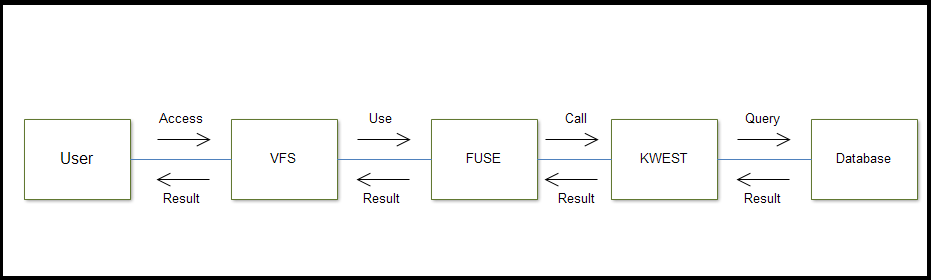
\includegraphics[width=0.8\textwidth]{comm.png}}
%\includegraphics[width=0.8\textwidth]{image.png}
%\caption{Communication diagram}
%\label{fig:commdiag}
%\end{figure}

\newpage
\subsection {Component diagram}
\vspace*{1.5cm}
\begin{figure}[htb]
\centering
\setlength\fboxsep{0pt}
\setlength\fboxrule{0.5pt}
\fbox{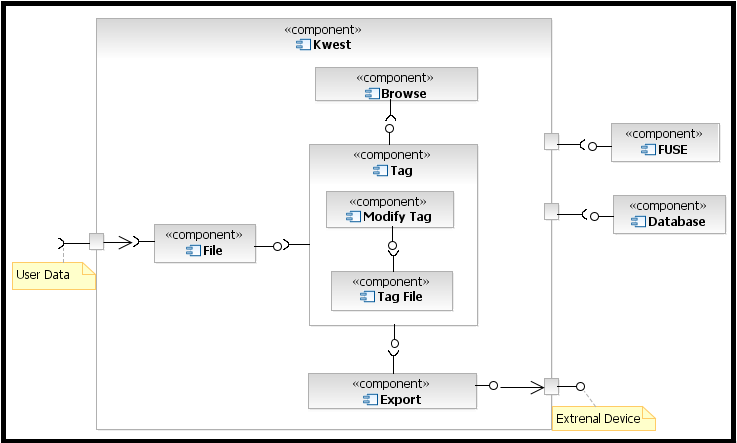
\includegraphics[width=1.0\linewidth]{./diagrams/comp.png}}
%\includegraphics[width=0.8\textwidth]{image.png}
\caption{Component diagram}
\label{fig:compdiag}
\end{figure}

\newpage
\subsection {Deployment diagram}
\vspace*{1.0cm}
\begin{figure}[htb]
\centering
\setlength\fboxsep{0pt}
\setlength\fboxrule{0.5pt}
\fbox{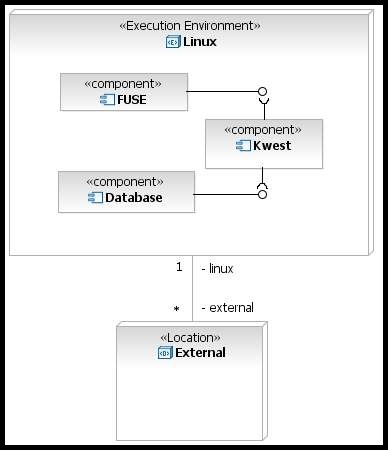
\includegraphics[width=1.0\linewidth]{./diagrams/deploy.png}}
%\includegraphics[width=0.8\textwidth]{image.png}
\caption{Deployment diagram}
\label{fig:deploydiag}
\end{figure}


\chapter {TECHNICAL SPECIFICATIONS}
\section {Development}
\subsection {FUSE}
For developing and managing the virtual filesystem we have used FUSE. It is a loadable kernel module for Unix-like computer operating systems that lets non-privileged users create their own file systems without editing kernel code. This is achieved by running file system code in user space while the FUSE module provides only a \textit{bridge} to the actual kernel interfaces. \newline
\emph{Minimum required: 2.8} \newline
\emph{Version used: 2.9.0} from \emph{http://fuse.sourceforge.net/}

\subsection {SQLite}
We have used SQLite as the data repository for this project. SQLite is a relational database management system contained in a small C programming library. It implements a self-contained, zero-configuration, transactional SQL database engine which can be embedded in applications. \newline
\emph{Minimum required: 3.6} \newline
\emph{Version Used: 3.7.13} from \emph{http://www.sqlite.org/}

\subsection {Language for Implementation}
We use ANSI C for implementing our project modules. Specifically, we follow the \textit{GNU C99} standards while compiling our code. GNU C99 is an extension of the C99 providing some extra features. \emph{Note:} Some features are incompatible with other standards. \newline
\emph{GNU C99} from \emph{http://gcc.gnu.org/c99status.html}

\subsection {Compiler}
For compiling our project modules we use the GNU Compiler Collection (GCC). GCC is a compiler system which provides front ends for various languages including C. It provides optimizations, debugging and other features to help program development. \newline
\emph{Minimum required: 4.6} \newline
\emph{Version used: 4.7.2} on \emph{Linux Mint 14}

\section {Operating Environment}
\subsection {Platform}
The project is based on operating systems utilising the linux kernel. Any implementation which provides a POSIX compatible enviroment is sufficient. \newline
\emph{Minimum required: 2.6.14} \newline
\emph{Version used: 3.5.0-generic} on \emph{Linux Mint 14}

\subsection {Operating System}
We have used various operating environments while creating and testing the project. Linux distributions were \emph{Ubuntu 12.04, Ubuntu 12.10, Fedora 18, Linux Mint 13, Linux Mint 14}.

\section {External Libraries}
\subsection{TagLib}
TagLib is a library for reading and editing the meta-data of several popular audio formats. Currently it supports both ID3v1 and ID3v2 for MP3 files, Ogg Vorbis comments and ID3 tags and Vorbis comments in FLAC, MPC, Speex, WavPack TrueAudio, WAV, AIFF, MP4 and ASF files. \newline
\emph{Minimum required: TagLib 1.7.1} \newline
\emph{Version used: TagLib 1.8} from \emph{http://taglib.github.com/}

\subsection{LibExtractor}
GNU Libextractor is a library used to extract meta data from files. The goal is to provide developers of file-sharing networks, browsers or WWW-indexing bots with a universal library to obtain simple keywords and meta data to match against queries and to show to users instead of only relying on filenames.  \newline
\emph{Minimum required: 1.0.0} \newline
\emph{Version used: 1.0.1} from \emph{http://www.gnu.org/software/libextractor/}

\subsection{Poppler}
Poppler is a PDF rendering library based on the xpdf-3.0 code base. \newline
\emph{Minimum required: 0.21} \newline
\emph{Version used: 0.22} from \emph{http://poppler.freedesktop.org/}


\section{Debugging}
\subsection{GDB: GNU Project Debugger}
GDB, the GNU Project debugger, allows you to see what is going on `inside' another program while it executes -- or what another program was doing at the moment it crashed. \newline
\emph{Version used: 7.5} from \emph{http://www.gnu.org/software/gdb/}

\subsection{Valgrind}
Valgrind is a GPL licensed programming tool for memory debugging, memory leak detection, and profiling. Valgrind was originally designed to be a free memory debugging tool for Linux on x86, but has since evolved to become a generic framework for creating dynamic analysis tools such as checkers and profilers. \newline
\emph{Version used: 3.7.0} from \emph{http://valgrind.org/}

\chapter{PROJECT ESTIMATION, SCHEDULE and TEAM STRUCTURE}
\section{Team Structure}
\subsection{Member 1: Aseem Gogte}
Prior Experience:
\begin{itemize}
\item Well versed in C, C++
\item Visual Basic
\item Java
\item Databases
\end{itemize}

\subsection{Member 2: Sahil Gupta}
Prior Experience:
\begin{itemize}
\item Well versed in C, C++
\item Visual Basic
\item Java
\item Databases
\end{itemize}

\subsection{Member 3: Harshvardhan Pandit}
Prior Experience:
\begin{itemize}
\item C/C++
\item Visual Basic
\item Java
\item System programming
\end{itemize}

\subsection{Member 4: Rohit Sharma}
Prior Experience:
\begin{itemize}
\item C/C++
\item Visual Basic
\item Java
\item Databases
\end{itemize}

\section{Work Breakdown Structure}
We also used the \emph{Work Breakdown Structure(WBS)} to compute the task breakdown associated with this project. The WBS modules are as follows: \newline
\begin{table}[h]
\begin{tabular}{|p{1cm}|p{10cm}|p{1cm}|}
\hline
\textbf{1} 	& \textbf{Project Management} & \textbf{5\%} \\ \hline
\indent 1.1	& Project Initiation & 1\% \\
1.2	& Project Planning & 1\% \\
1.3	& Project Execution and Control & 2\% \\
1.4	& Project Closeout & 1\% \\ \hline
\textbf{2}	& \textbf{Definition} & \textbf{10\%} \\ \hline
2.1	& Start-up and Orientation & 2\% \\
2.2	& Determine Project Requirements & 2\% \\
2.3	& Create future process model & 1\% \\
2.4	& Reconcile Project Requirements & 1\% \\
2.5	& Functional Specification & 4\% \\ \hline
\textbf{3}	& \textbf{System Design} & \textbf{20\%} \\ \hline
3.1	& Technical Architecture  & 5\% \\ 
3.2	& System Standards & 2\% \\ 
3.3	& Physical Environment & 2\% \\ 
3.4	& Technical Specification & 3\% \\ 
3.5	& Creating Prototypes & 5\% \\ 
3.6	& Test Plans & 3\% \\ \hline
\textbf{4}	& \textbf{System Development} & \textbf{40\%} \\ \hline
4.1	& Develop and Test Software Modules & 10\% \\ 
4.2	& User Training Materials & 2\% \\ 
4.3	& Technical Documentation & 8\% \\ 
4.4	& Unit, Integration and System Test Results & 10\% \\ 
4.5	& Performance testing & 5\% \\ 
4.6	& Acceptance testing & 5\% \\ \hline
\textbf{5} & \textbf{System Implementation} & \textbf{20\%} \\ \hline
5.1	& Acceptance Environment & 5\% \\ 
5.2	& Data Initialisation and Conversion Test Results & 8\% \\ 
5.3	& Acceptance test results & 3\% \\ 
5.4	& Supporting Material & 4\% \\ \hline
\textbf{6} & \textbf{Transition to Ready State} & \textbf{5\%} \\ \hline
6.1	& Train Users & 1\% \\ 
6.2	& Convert Data & 1\% \\ 
6.3	& Deploy System & 3\% \\ \hline
\end{tabular}
\caption{Work Breakdown Structure}
\label{tag:WBS}
\end{table}



\chapter{SOFTWARE IMPLEMENTATION}
\section{Introduction}
The implementation of the software was done in a modular manner using the incremental approach of SDLC. ANSI C was the language used to implement the project. An SQLite database was used for creating and managing the data repository. Various external libraries were used for the extraction of the metadata. The following modules constituted our project:
\begin{list}{•}{•}
\item \textbf{Module 1:} Creation of a virtual file system using FUSE
\item \textbf{Module 2:} Interfacing a Data Repository using SQLite
\item \textbf{Module 3:} Adding automated Extraction of Metadata 
\item \textbf{Module 4:} Importing Semantics in to the file system
\item \textbf{Module 5:} Exporting Semantics from the file system
\item \textbf{Module 6:} Association Rule learning using Apriori Algorithm
\end{list}

\section{Creation of a virtual file system using FUSE}

The first module of implementation was to create a basic file system using FUSE. Using FUSE we created a virtual file system capable of doing all the operations that a normal file system does.
The module consists of the following phases:
\begin{list}{•}{•}

\item \textbf{Phase 1:} Implement FUSE to create a basic file system structure using ANSI C as the implementation language.

\item \textbf{Phase 2:} Connect the file system created to the data repository created using a SQLite database. Create tags and files view by querying the database through FUSE.

\item \textbf{Phase 3:} Implementing common file operations with respect to tags and files such as read, write, open, copy, move etc.

\item \textbf{Phase 4:} Extraction of metadata from the files using external libraries and organisation of the file system based on metadata.

\item \textbf{Phase 5:} Displaying suggestion based on associations derived using Apriori Algorithm. 
\end{list}

\section{Interfacing a Data Repository using SQLite}
The project was to implement a semantic file system. This required a data repository to store all the information such as file name, physical location, attributes, etc. Also, the metadata extracted from the files was also stored in the database. Thus, the database formed a central information location for the file system.


It is vital for the proper functioning of the system that the database always remains consistent. Logging mechanisms ensure that operations on the database always reach an endpoint. This module is used to check, correct and maintain integrity of the database by checking for redundant entries. Also, if there are new files which have not been added to KWEST, this module can help the user add them.


The database is an important module of the file system. All the data required to browse and navigate the file system is stored in the database. FUSE interacts with the data in the database by querying for particular data based on path accessed. We implement this module in the following ways:
\begin{list}{•}{•}
\item \textbf{Phase 1:} Create database tables for a file system.
\item \textbf{Phase 2:} The relation tables between tags, files are stored.
\item \textbf{Phase 3:} Store the extracted metadata in the database.
\item \textbf{Phase 4:} The association rules for the data are derived using the Apriori algorithm.
\end{list}

\section{Adding automated Extraction of Metadata}
Metadata (meta content) is defined as data providing information about one or more aspects of the data. Metadata can be stored either internally, in the same file as the data, or externally, in a separate file. Metadata that is embedded with content is called embedded metadata.
The metadata of the file is extracted by using external libraries. The data repository stores the extracted metadata in a predetermined format. 
\begin{list}{•}{•}
\item \textbf{Phase 1:} Test external libraries to determine which of them can be used.
\item \textbf{Phase 2:} Extract metadata using external libraries.
\item \textbf{Phase 3:} Store the extracted metadata in the database.
\item \textbf{Phase 4:} Form relations between metadata and files using association rules.
\end{list}

\section{Importing Semantics in to the file system}
Users already have certain organisational structures in the way they store data in file systems. This module imports semantics by converting the storage hierarchy to tag-based hierarchy. This means the directory structure present in the file system will be used to form tags and the files listed under the directory are tagged under that tag.
\begin{list}{•}{•}
\item \textbf{Phase 1:} Parse the folder structure on local hard disk.
\item \textbf{Phase 2:} Add entry for each file and folder to the database.
\item \textbf{Phase 3:} Remove or ignore hidden and system files.
\item \textbf{Phase 4:} Prune the database entries on every start up.
\end{list}
\newpage
\section{Exporting Semantics from the file system}
This module can export the storage hierarchy to some external location. The semantic organisation of tags is converted to actual directories and the files are then copied to these directories. This is similar to copying contents from one file system to another.
\begin{list}{•}{•}
\item \textbf{Phase 1:} Copy virtual locations to external location.
\item \textbf{Phase 2:} Perform physical copy of files.
\item \textbf{Phase 3:} Create folders and sub folders based on tags.
\item \textbf{Phase 4:} Copy suggestions using data repository.
\end{list}

\section{Association Rule learning using Apriori Algorithm}
Association rules help in organising the file system data by providing suggestions while tagging files. These suggestions can be helpful when the user has either forgotten to tag the file, or is yet about to do it. This association rule learning approach uses the Apriori algorithm.
\begin{list}{•}{•}
\item \textbf{Phase 1:} Run Apriori over the KWEST database.
\item \textbf{Phase 2:} Perform optimisation's and prune steps.
\item \textbf{Phase 3:} Store association rules in database.
\item \textbf{Phase 4:} Integrate with KWEST to show suggestions.
\end{list}

\chapter {SOFTWARE TESTING}
\section{Introduction}
\subsection{Purpose}
Software testing can be stated as the process of validating and verifying that a computer program/application/product:
\begin{itemize}
\item Meets the requirements that guided its design and development.
\item Works as expected.
\item Can be implemented with the same characteristics.
\item Satisfies the needs of stakeholders.
\end{itemize}

Software testing, depending on the testing method employed, can be implemented at any time in the development process. Traditionally most of the test effort occurs after the requirements have been defined and the coding process has been completed, but in the Agile approaches most of the test effort is on-going. As such, the methodology of the test is governed by the chosen software development methodology.

\subsection{Scope}
The testing of the system was done manually and no testing tools were used. The \emph{test plan} describes the \emph{unit, functional, performance, usability, regression} tests that were performed. Only codes that were pushed as commits were considered as candidates for testing.

\subsection{Intended Audience}
The testing of this system is intended for 3 types of audiences:
\begin{enumerate}
\item \textbf{End Users:} The users who will be using the system will review the testing as a mark of stability and performance of the system.
\item \textbf{Developers:} Will view the testing for knowing existing limitations and bugs.
\item \textbf{Reviewers:} Will use these test results as a metric to evaluate the project.
\end{enumerate}

\section{Test Plan}
\subsection{Target Items}
The following have been identified as targets for testing:
\begin{enumerate}
\item Code and associated areas
\item File system operations
\item Databases: SQLite3
\item Operating Systems
\end{enumerate}

\subsection{Outline of Tests}
\subsection*{Tests performed}
\begin{enumerate}
\item Performance tests
\item Functional tests
\item Data Integrity tests
\item Regression tests
\item Usability tests
\end{enumerate}

\subsection{Test Approach}
Any bugs found should be reported with related information, which should include
who discovered it, how, a description of the bug, and who fixed it and
when. Also, re-testing of the code done to make sure that defect has been fixed
and there no new bugs produced due to change in code.

\begin{enumerate}
\item \textbf{Performance Testing:} \\
The focus of Performance testing is checking a software program’s
\begin{itemize}
\item \emph{Speed} : Determines whether the system responds quickly.
\item \emph{Scalability} : Determines maximum user load the software application can handle.
\item \emph{Stability} : Determines if the application is stable under varying loads.
\end{itemize}
\textbf{Tools required:} Software timers \\
\textbf{Success criteria:} 
\begin{enumerate}
\item Manual(user) perception does not notice any ``lags''.
\item Time to perform operations is within an acceptable range.
\end{enumerate}


\item \textbf{Functional Testing:} \\
The prime objective of Functional testing is   checking the functionalities of the software system. It mainly concentrates on -
\begin{itemize}
\item \emph{Mainline functions} :  Testing the main functions of an application.
\item \emph{Basic Usability} : It involves basic usability testing of the system. It checks whether an user can freely navigate through the screens without any difficulties.
\item \emph{Accessibility} :  Checks the accessibility of the system for the user.
\item \emph{Error Conditions} : Usage of testing techniques to check for error conditions.  It checks whether suitable error messages are displayed.
\end{itemize}
\textbf{Tools required:} None(manual testing) \\
\textbf{Success criteria:} All of the following are successfully tested:
\begin{enumerate}
\item all key use-case scenarios.
\item all key features.
\end{enumerate}

\item \textbf{Data Integrity Testing:} \\
Data integrity refers to the quality of the data in databases and is the measurement by which users examine data quality, reliability and usefulness. Data integrity testing verifies that converted data is accurate and functions correctly within a given application. Testing data integrity involves:
\begin{itemize}
\item \textbf{Database} : Verifying that correct values are saved in databases.
\item \textbf{Write-back} : Correct data is written to disk.
\item \textbf{Read} : Correct data is read from disk.
\item \textbf{File Integrity} : Operations do not break existing files.
\end{itemize}
\textbf{Tools required:} File compare tools (manual testing) \\
\textbf{Success criteria:} All of the following are successfully tested:
\begin{enumerate}
\item files are same in size, byte-blocks, permissions and parameters.
\item data is not changed, modified or removed unless intended.
\end{enumerate}

\item \textbf{Regression Testing:} \\
Regression Testing is required when there is a :
\begin{itemize}
\item Change in requirements and code is modified according to the requirement
\item New feature is added to the software
\item Defect fixing
\item Performance issue fix 
\end{itemize}
\textbf{Tools required:} None(manual testing) \\
\textbf{Success criteria:} All of the following are successfully tested:
\begin{enumerate}
\item all previous operations are successfully executed.
\item previously solved bugs are not re-introduced.
\item operations do not suffer from unwanted performance hits.
\end{enumerate}

\item \textbf{Usability Testing:} \\
Goal of this testing is to satisfy users and it mainly concentrates on the following parameters of a system: \\
\textbf{Effectiveness of the system}
\begin{itemize}
\item Is the system is easy to learn?
\item Is the system useful and adds value to the target audience?
\item Is Content, Colour, Icons, Images used are aesthetically pleasing ?
\end{itemize}
\textbf{Efficiency}
\begin{itemize}
\item Navigation required to reach desired screen/web page should be very less. Scroll bars shouldn’t be used frequently.
\item Uniformity in the format of screen/pages in your application/website.
\item Provision to search within your software application or website
\end{itemize}
\textbf{Accuracy}
\begin{itemize}
\item No outdated or incorrect data like contact information/address should be present.
\item No broken links should be present.
\item User Friendliness
\item Controls used should be self-explanatory and must not require training to operate
\item Help should be provided for the users to understand the application / website
\item Alignment with above goals helps in effective usability testing
\end{itemize}
\textbf{Tools required:} None(manual testing) \\
\textbf{Success criteria:} All of the following are successfully tested:
\begin{enumerate}
\item operations are not changed drastically from a traditional file system.
\item user can use the file system without any special tools.
\end{enumerate}
\end{enumerate}

\subsection{Entry and Exit Criteria:}

\begin{enumerate}
\item Test Plan
\begin{enumerate}[label=\Alph*]
\item \textbf{Test Plan Entry Criteria:} Code is complete and has been pushed to the Git repository.
\item \textbf{Test Plan Exit Criteria:} All functional requirements have been verified.
\item \textbf{Suspension and Resumption Criteria:} Testing will be suspended on critical
design flaws that will changes in redesign of critical components. Testing will resume when the coding is complete and code is reviewed successfully.
\end{enumerate}

\item Test Cycle
\begin{enumerate}[label=\Alph*]
\item \textbf{Test Cycle Entry Criteria:} When a module has been completed.
\item\textbf{ Test Cycle Exit Criteria:} All tests specified at the start of the testing have
completed successfully.
\end{enumerate}
\end{enumerate}

\subsection{Risks, Dependencies, Assumptions, Constraints}
\begin{table}[h]
\begin{tabular}{|p{2cm}|p{8cm}|p{4cm}|}
\hline
\textbf{Risk} & \textbf{Mitigation Strategy} & \textbf{Contingency} \\ \hline
FUSE API changes & Use FUSE version numbers to run a static check while compiling for required version of FUSE. & Change operation code to new version. \\ \hline
External Library is no longer maintained & Try to use the latest version number of library available and keep a source ready for distribution. & Change to alternate library. \\ \hline
Performance has degraded & Code with performance in mind, using fast algorithms and approaches. & Use profiling tools to detect memory issues and static code analysers for code checking. \\
\hline
\end{tabular}
\caption{Risk Management}
\label{tab: risk}
\end{table}

\subsection{Problem Reporting, Escalation, and Issue Resolution}
Each bug will be given a priority, which will determine when it is addressed in the current iteration. The bug priority may change due to other bugs, issues or re-evaluation of the bug by a peer review.

\section{Test Cases}
\subsection{Introduction}
The purpose of this Test Case document is to specify and communicate the specific
conditions which need to be validated to enable an assessment of the system. Test
Cases are motivated by many things but will usually include a subset of Use Cases,
performance characteristics and the risks the project is concerned with.
A separate test case document is prepared for each testing phase (unit,
integration, integrity, etc.) identified in the test plan. The test cases should be
organised into related groups that are meaningful to the project – i.e. test suites.

\subsection{File System Operations}
Testing the file system for implementations of required operations:
\begin{table}[h]
\begin{tabular}{|p{2cm}|p{2cm}|p{8cm}|}
\hline
\textbf{Operation} & \textbf{Status} & \textbf{Comment} \\ \hline
getattr & YES & checks whether the given path exits \\
readdir	 & YES & lists the contents of the given tag \\
access	& YES & checks for access to specified tag \\
truncate	 & YES & closes file after operation \\
destroy	 & YES & called on file system unmount \\
open		& YES & opens for file for access \\
release	& YES & releases file after access \\
mknod		& YES & creates new file \\
rename		& YES & renames files and folders \\
unlink		& YES & removes file from system \\
read		& YES & reads data from file \\
write		& YES & writes data to file \\
chmod		& YES & changes permissions \\
chown		& YES & changes owner\\
mkdir		& YES & creates new directory \\
rmdir		& YES & removes directory\\

symlink	 & INVALID & not required in KWEST \\ 
readlink & INVALID & not required in KWEST \\
link		& INVALID & not required in KWEST \\
utimens	& NO & not implemented \\
statfs	& NO & not implemented \\
fsync & INVALID & not required in KWEST \\

setxattr	& NO & not implemented \\
getxattr	& NO & not implemented \\
listxattr	& NO & not implemented \\
removexattr	& NO & not implemented \\
\hline
\end{tabular}
\caption{File system operations}
\label{fsop}
\end{table}

\subsection{Performance of file system operations}
Comparison of KWEST file system against underlying file system.
\textbf{Test Bench:}
\begin{itemize}
\item Operating System: Linux Mint 14 3.5.0-25-generic
\item Original file system: ext4 500GB disk with partition size 150GB
\item RAM: 4GB
\item swap: 8GB on disk
\item CPU utilisation: average 4%
\end{itemize}
\textbf{Contents of Music folder imported into KWEST:}
\begin{itemize}
\item \textbf{Audio:} 17 files totalling 102.9MB
\item \textbf{Images:} 81 files totalling 196MB
\item \textbf{PDF:} 11 files totalling 17.9MB
\item \textbf{Video:} 4 files totalling 1GB
\item \textbf{Others:} 7 files totalling 7MB
\item \textbf{Total:} 120 files of size 1.3GB
\end{itemize}

\begin{table}[h]
\begin{tabular}{|p{3cm}|p{2cm}|p{7cm}|}
\hline
\textbf{Test} & \textbf{Time taken} & \textbf{Comment} \\ \hline
all files	&	120sec	& total file size imported was 1.3GB \\ \hline
videos	& 40sec	&	extracting metadata from videos is more expensive compared to other file types \\ \hline
images	& 35sec & images having metadata take longer than those without \\ \hline
audio 	& 4sec	& audio files are the fastest to parse and load \\ \hline
PDF		& 2sec	& PDF files are parsed quickly as compared to other document types \\ \hline
forming associations & 2sec	 & time is proportional to number of common files in user tags \\
\hline
\end{tabular}
\caption{Performance tests for mounting KWEST}
\label{performancemount}
\end{table}

\textbf{Test Script:} The following is a simple test script used to evaluate file system operations. The script works by calculating the difference in time before and after the execution of operations.
\begin{lstlisting}[language=bash,frame=single]
#store current time
let DA=(`date +%s `)
#perform file system operation
ls -R kwest/src/mnt
#store new time
let DB=(`date +%s`)
#calculate the difference
let DC=$DB-$DA
#output the time taken
echo $DC
\end{lstlisting}

\begin{table}[h]
\begin{tabular}{|p{2cm}|p{1.5cm}|p{1.5cm}|p{7cm}|}
\hline
\textbf{Operation} & \textbf{ext4} & \textbf{KWEST} & \textbf{Comment} \\ \hline
list directory	&	500ms	&	550ms & there is no noticeable difference \\ \hline
read file	&	700ms & 850ms	& some extra time is taken to read a file depending on the amount of data being read. In general, there is no noticeable difference. \\ \hline
write file	&	1200ms & 2200ms	& (for 5MB text file) writing takes slightly more time, but the difference is within acceptable range. \\ \hline
read and write	&	1010ms & 2400ms & (for 5MB text file) reading and writing simultaneously does not produce any performance degradation. \\
\hline
\end{tabular}
\caption{Performance tests for using KWEST}
\label{performancetests}
\end{table}

\subsection{Profiling Code}
Code can be profiled using Manual methods, or using specific tools such as Valgrind, GDB, Splint etc. For testing KWEST, we have used the following profiling tools:
\subsection*{GDB}
GDB can be used to debug the file system and check for memory leaks, errors and irregular operations. The sample output given below shows a clean mount and unmount of the KWEST file system.
\begin{lstlisting}[language=bash,frame=single]
$ gdb ./kwest
GNU gdb (GDB) 7.5-ubuntu
Copyright (C) 2012 Free Software Foundation, Inc.
License GPLv3+: GNU GPL version 3 or later 
<http://gnu.org/licenses/gpl.html>
This is free software: you are free to change and redistribute it.
There is NO WARRANTY, to the extent permitted by law.  
Type `show copying` and `show warranty` to see details.
This GDB was configured as "x86_64-linux-gnu".
For bug reporting instructions, please see:
<http://www.gnu.org/software/gdb/bugs/>...
Reading symbols from kwest/src/kwest....
(gdb) run -s -d -f mnt
Starting program: kwest/src/kwest -s -d -f mnt
[Thread debugging using libthread_db enabled]
Using host libthread_db library "/lib/x86_64-linux-gnu/libthread_db.so.1".
KWEST - A Semantically Tagged Virtual File System
...
...
[Inferior 1 (process 20863) exited normally]
(gdb) bt
No stack.
\end{lstlisting}

\begin{table}[h]
\begin{tabular}{|p{3cm}|p{2cm}|p{8cm}|}
\hline
\textbf{Test} & \textbf{Status} & \textbf{Possible Errors} \\ \hline
list directory	&	PASS &  I/O error, illegal operation, transport endpoint not connection, connection abort \\ \hline
read file & PASS & I/O error, illegal operation, access denied, database error \\ \hline
write file & PASS & I/O error, illegal operation, access denied, file system busy \\ \hline
mknod & PASS & Operation not permitted, I/O error, database error \\ \hline
unlink & PASS & Device busy, Operation not permitted, I/O error, database error \\ \hline
mkdir & PASS & Operation not permitted, I/O error, database error \\ \hline
rmdir & PASS & Device busy, Operation not permitted, I/O error, database error \\ \hline
chmod & PASS & Access denied, I/O error, device busy, database error \\ \hline
associations & PASS & memory error, segmentation fault, unconditional jump, I/O error \\ \hline
fuse main & PASS & incompatible version \\
\hline
\end{tabular}
\caption{GDB debugging for KWEST}
\label{tab:GDB}
\end{table}

\chapter {RESULTS}
\section{Introduction}
\subsection{Purpose}
Software testing can be stated as the process of validating and verifying that a computer program/application/product:
\begin{itemize}
\item Meets the requirements that guided its design and development.
\item Works as expected.
\item Can be implemented with the same characteristics.
\item Satisfies the needs of stakeholders.
\end{itemize}

Software testing, depending on the testing method employed, can be implemented at any time in the development process. Traditionally most of the test effort occurs after the requirements have been defined and the coding process has been completed, but in the Agile approaches most of the test effort is on-going. As such, the methodology of the test is governed by the chosen software development methodology.

\subsection{Scope}
The testing of the system was done manually and no testing tools were used. The \emph{test plan} describes the \emph{unit, functional, performance, usability, regression} tests that were performed. Only codes that were pushed as commits were considered as candidates for testing.

\subsection{Intended Audience}
The testing of this system is intended for 3 types of audiences:
\begin{enumerate}
\item \textbf{End Users:} The users who will be using the system will review the testing as a mark of stability and performance of the system.
\item \textbf{Developers:} Will view the testing for knowing existing limitations and bugs.
\item \textbf{Reviewers:} Will use these test results as a metric to evaluate the project.
\end{enumerate}

\section{Test Plan}
\subsection{Target Items}
The following have been identified as targets for testing:
\begin{enumerate}
\item Code and associated areas
\item Filesystem operations
\item Databases: SQLite3
\item Operating Systems
\end{enumerate}

\subsection{Outline of Tests}
\subsection*{Tests performed}
\begin{enumerate}
\item Performance tests
\item Functional tests
\item Data Integrity tests
\item Regression tests
\item Usability tests
\end{enumerate}

\subsection{Test Approach}
Any bugs found should be reported with related information, which should include
who discovered it, how, a description of the bug, and who fixed it and
when. Also, re-testing of the code done to make sure that defect has been fixed
and there no new bugs produced due to change in code.

\begin{enumerate}
\item \textbf{Performance Testing:} \\
The focus of Performance testing is checking a software program’s
\begin{itemize}
\item \emph{Speed} : Determines whether the system responds quickly.
\item \emph{Scalability} : Determines maximum user load the software application can handle.
\item \emph{Stability} : Determines if the application is stable under varying loads.
\end{itemize}
\textbf{Tools required:} Software timers \\
\textbf{Success criteria:} 
\begin{enumerate}
\item Manual(user) perception does not notice any ``lags''.
\item Time to perform operations is within an acceptable range.
\end{enumerate}


\item \textbf{Functional Testing:} \\
The prime objective of Functional testing is   checking the functionalities of the software system. It mainly concentrates on -
\begin{itemize}
\item \emph{Mainline functions} :  Testing the main functions of an application.
\item \emph{Basic Usability} : It involves basic usability testing of the system. It checks whether an user can freely navigate through the screens without any difficulties.
\item \emph{Accessibility} :  Checks the accessibility of the system for the user.
\item \emph{Error Conditions} : Usage of testing techniques to check for error conditions.  It checks whether suitable error messages are displayed.
\end{itemize}
\textbf{Tools required:} None(manual testing) \\
\textbf{Success criteria:} All of the following are successfully tested:
\begin{enumerate}
\item all key use-case scenarios.
\item all key features.
\end{enumerate}

\item \textbf{Data Integrity Testing:} \\
Data integrity refers to the quality of the data in databases and is the measurement by which users examine data quality, reliability and usefulness. Data integrity testing verifies that converted data is accurate and functions correctly within a given application. Testing data integrity involves:
\begin{itemize}
\item \textbf{Database} : Verifying that correct values are saved in databases.
\item \textbf{Write-back} : Correct data is written to disk.
\item \textbf{Read} : Correct data is read from disk.
\item \textbf{File Integrity} : Operations do not break existing files.
\end{itemize}
\textbf{Tools required:} File compare tools (manual testing) \\
\textbf{Success criteria:} All of the following are successfully tested:
\begin{enumerate}
\item files are same in size, byte-blocks, permissions and parameters.
\item data is not changed, modified or removed unless intended.
\end{enumerate}

\item \textbf{Regression Testing:} \\
Regression Testing is required when there is a :
\begin{itemize}
\item Change in requirements and code is modified according to the requirement
\item New feature is added to the software
\item Defect fixing
\item Performance issue fix 
\end{itemize}
\textbf{Tools required:} None(manual testing) \\
\textbf{Success criteria:} All of the following are successfully tested:
\begin{enumerate}
\item all previous operations are successfully executed.
\item previously sovled bugs are not re-introduced.
\item operations do not suffer from unwanted performance hits.
\end{enumerate}

\item \textbf{Usability Testing:} \\
Goal of this testing is to satisfy users and it mainly concentrates on the following parameters of a system: \\
\textbf{Effectiveness of the system}
\begin{itemize}
\item Is the system is easy to learn?
\item Is the system useful and adds value to the target audience?
\item Is Content, Color, Icons, Images used are aesthetically pleasing ?
\end{itemize}
\textbf{Efficiency}
\begin{itemize}
\item Navigation required to reach desired screen/webpage should be very less. Scroll bars shouldn’t be used frequently.
\item Uniformity in the format of screen/pages in your application/website.
\item Provision to search within your software application or website
\end{itemize}
\textbf{Accuracy}
\begin{itemize}
\item No outdated or incorrect data like contact information/address should be present.
\item No broken links should be present.
\item User Friendliness
\item Controls used should be self-explanatory and must not require training to operate
\item Help should be provided for the users to understand the application / website
\item Alignment with above goals helps in effective usability testing
\end{itemize}
\textbf{Tools required:} None(manual testing) \\
\textbf{Success criteria:} All of the following are successfully tested:
\begin{enumerate}
\item operations are not changed drastically from a traditional file sytem.
\item user can use the file system without any special tools.
\end{enumerate}
\end{enumerate}

\subsection{Entry and Exit Criteria:}

\begin{enumerate}
\item Test Plan
\begin{enumerate}[label=\Alph*]
\item \textbf{Test Plan Entry Criteria:} Code is complete and has been pushed to the Git repository.
\item \textbf{Test Plan Exit Criteria:} All functional requirments have been verified.
\item \textbf{Suspension and Resumption Criteria:} Testing will be suspended on critical
design flaws that will changes in redesign of critical components. Testing will resume when the coding is complete and code is reviewed successfully.
\end{enumerate}

\item Test Cycle
\begin{enumerate}[label=\Alph*]
\item \textbf{Test Cycle Entry Criteria:} When a module has been completed.
\item\textbf{ Test Cycle Exit Criteria:} All tests specified at the start of the testing have
completed successfully.
\end{enumerate}
\end{enumerate}

\subsection{Risks, Dependencies, Assumptions, Constraints}
\begin{table}[h]
\begin{tabular}{|p{2cm}|p{8cm}|p{4cm}|}
\hline
\textbf{Risk} & \textbf{Mitigation Strategy} & \textbf{Contingency} \\ \hline \hline
FUSE API changes & Use FUSE version numbers to run a static check while compiling for required version of FUSE. & Change operation code to new version. \\ \hline
External Library is no longer maintained & Try to use the latest version number of library available and keep a source ready for distribution. & Change to alternatice library. \\ \hline
Performance has degraded & Code with performance in mind, using fast algorithms and approaches. & Use profiling tools to detect memory issues and static code analysers for code checking. \\
\hline
\end{tabular}
\caption{Risk Management}
\label{tab: risk}
\end{table}

\subsection{Problem Reporting, Escalation, and Issue Resolution}
Each bug will be given a priority, which will determine when it is addressed in the current iteration. The bug priority may change due to other bugs, issues or re-evaluation of the bug by a peer review.

\section{Test Cases}
\subsection{Introduction}
The purpose of this Test Case document is to specify and communicate the specific
conditions which need to be validated to enable an assessment of the system. Test
Cases are motivated by many things but will usually include a subset of Use Cases,
performance characteristics and the risks the project is concerned with.
A separate test case document is prepared for each testing phase (unit,
integration, integrity, etc.) identified in the test plan. The test cases should be
organized into related groups that are meaningful to the project – i.e. test suites.

\subsection{File System Operations}
Testing the file system for implementations of required operations:
\begin{table}[h]
\begin{tabular}{|p{2cm}|p{2cm}|p{8cm}|}
\hline
\textbf{Operation} & \textbf{Status} & \textbf{Comment} \\ \hline
getattr & YES & checks whether the given path exits \\
readdir	 & YES & lists the contents of the given tag \\
access	& YES & checks for access to specified tag \\
truncate	 & YES & closes file after operation \\
destroy	 & YES & called on file system unmount \\
open		& YES & opens for file for access \\
release	& YES & releses file after access \\
mknod		& YES & creates new file \\
rename		& YES & renames files and folders \\
unlink		& YES & removes file from system \\
read		& YES & reads data from file \\
write		& YES & writes data to file \\
chmod		& YES & changes permissions \\
chown		& YES & changes owner\\
mkdir		& YES & creates new directory \\
rmdir		& YES & removes directory\\

symlink	 & INVALID & not required in KWEST \\ 
readlink & INVALID & not required in KWEST \\
link		& INVALID & not required in KWEST \\
utimens	& NO & not implemented \\
statfs	& NO & not implemented \\
fsync & INVALID & not required in KWEST \\

setxattr	& NO & not implemented \\
getxattr	& NO & not implemented \\
listxattr	& NO & not implemented \\
removexattr	& NO & not implemented \\
\hline
\end{tabular}
\caption{File system operations}
\label{fsop}
\end{table}

\subsection{Performance of file system operations}
Comparison of KWEST file system against underlying file system.
\textbf{Test Bench:}
\begin{itemize}
\item Operating System: Linux Mint 14 3.5.0-25-generic
\item Original file system: ext4 500GB disk with partition size 150GB
\item RAM: 4GB
\item swap: 8GB on disk
\item CPU utilization: average 4%
\end{itemize}
\textbf{Contents of Music folder imported into KWEST:}
\begin{itemize}
\item \textbf{Audio:} 17 files totalling 102.9MB
\item \textbf{Images:} 81 files totalling 196MB
\item \textbf{PDF:} 11 files totalling 17.9MB
\item \textbf{Video:} 4 files totalling 1GB
\item \textbf{Others:} 7 files totalling 7MB
\item \textbf{Total:} 120 files of size 1.3GB
\end{itemize}

\begin{table}[h]
\begin{tabular}{|p{3cm}|p{2cm}|p{7cm}|}
\hline
\textbf{Test} & \textbf{Time taken} & \textbf{Comment} \\ \hline
all files	&	120sec	& total file size imported was 1.3GB \\ \hline
videos	& 40sec	&	extracting metadata from videos is more expensiv compared to other file types \\ \hline
images	& 35sec & images having metadata take longer than those without \\ \hline
audio 	& 4sec	& audio files are the fastest to parse and load \\ \hline
PDF		& 2sec	& PDF files are parsed quickly as compared to other document types \\ \hline
forming associations & 2sec	 & time is proportional to number of common files in user tags \\
\hline
\end{tabular}
\caption{Performance tests for mounting KWEST}
\label{performancemount}
\end{table}

\textbf{Test Script:} The following is a simple test script used to evaluate file system operations. The scipt works by calculating the difference in time before and after the execution of operations.
\begin{lstlisting}[language=bash,frame=single]
#store current time
let DA=(`date +%s `)
#perform file system operation
ls -R kwest/src/mnt
#store new time
let DB=(`date +%s`)
#calculate the difference
let DC=$DB-$DA
#output the time taken
echo $DC
\end{lstlisting}

\begin{table}[h]
\begin{tabular}{|p{2cm}|p{1.5cm}|p{1.5cm}|p{7cm}|}
\hline
\textbf{Operation} & \textbf{ext4} & \textbf{KWEST} & \textbf{Comment} \\ \hline
list directory	&	500ms	&	550ms & there is no noticiable difference \\ \hline
read file	&	700ms & 850ms	& some extra time is taken to read a file depending on the amount of data being read. In general, there is no noticiable difference. \\ \hline
write file	&	1200ms & 2200ms	& (for 5MB text file) writing takes slightly more time, but the difference is within acceptable range. \\ \hline
read and write	&	1010ms & 2400ms & (for 5MB text file) reading and writing simultaenously does not produce any performance degradation. \\
\hline
\end{tabular}
\caption{Performance tests for using KWEST}
\label{performancetests}
\end{table}

\subsection{Profiling Code}
Code can be profiled using Manual methods, or using specific tools such as Valgrind, GDB, Splint etc. For testing KWEST, we have used the following profiling tools:
\subsection*{GDB}
GDB can be used to debug the file systemand check for memory leaks, errors and irregular operations. The sample output given below shows a clean mount and unmount of the KWEST file system.
\begin{lstlisting}[language=bash,frame=single]
$ gdb ./kwest
GNU gdb (GDB) 7.5-ubuntu
Copyright (C) 2012 Free Software Foundation, Inc.
License GPLv3+: GNU GPL version 3 or later 
<http://gnu.org/licenses/gpl.html>
This is free software: you are free to change and redistribute it.
There is NO WARRANTY, to the extent permitted by law.  
Type `show copying` and `show warranty` to see details.
This GDB was configured as "x86_64-linux-gnu".
For bug reporting instructions, please see:
<http://www.gnu.org/software/gdb/bugs/>...
Reading symbols from kwest/src/kwest....
(gdb) run -s -d -f mnt
Starting program: kwest/src/kwest -s -d -f mnt
[Thread debugging using libthread_db enabled]
Using host libthread_db library "/lib/x86_64-linux-gnu/libthread_db.so.1".
KWEST - A Semantically Tagged Virtual File System
...
...
[Inferior 1 (process 20863) exited normally]
(gdb) bt
No stack.
\end{lstlisting}

\begin{table}[h]
\begin{tabular}{|p{3cm}|p{2cm}|p{8cm}|}
\hline
\textbf{Test} & \textbf{Status} & \textbf{Possible Errors} \\ \hline
list directory	&	PASS &  I/O error, illegal operation, transport endpoint not connection, connection abort \\ \hline
read file & PASS & I/O error, illegal operation, access denied, database error \\ \hline
write file & PASS & I/O error, illegal operation, access denied, file system busy \\ \hline
mknod & PASS & Operation not permitted, I/O error, database error \\ \hline
unlink & PASS & Device busy, Operation not permitted, I/O error, database error \\ \hline
mkdir & PASS & Operation not permitted, I/O error, database error \\ \hline
rmdir & PASS & Device busy, Operation not permitted, I/O error, database error \\ \hline
chmod & PASS & Access denied, I/O error, device busy, database error \\ \hline
associations & PASS & memory error, segmentation fault, unconditional jump, I/O error \\ \hline
fuse main & PASS & incompatible version \\
\hline
\end{tabular}
\caption{GDB debugging for KWEST}
\label{tab:GDB}
\end{table}

\chapter{DEPLOYMENT AND MAINTAINENCE}

\section{Installation and Uninstallaion}
\subsection{Installing}
\begin{itemize}
\item Get the latest copy of KWEST by downloading from the project hosting site: \url{https://code.google.com/p/kwest/downloads}
\item After extracting the contents, open up a terminal and type in the following commands:
\begin{lstlisting}[language=bash,frame=single]
make kwest_libs
export LD_LIBRARY_PATH=../lib:D_LIBRARY_PATH
make
\end{lstlisting}
\end{itemize}

\subsection{Mounting and Unmounting}
\begin{itemize}
\item To mount a KWEST file system, the user needs to run the \textit{mount} script which will mount the file system in the specified folder. 
\begin{lstlisting}[language=bash,frame=single]
./kwest mount-point
\end{lstlisting}
\item To unmount a KWEST file system, the user needs to run the \textit{fusermount -u} command with the argument \textit{path of KWEST mount point}. A successful unmount operation does not return any message.
\begin{lstlisting}[language=bash,frame=single]
fusermount -u mount-point
\end{lstlisting}
\end{itemize}

\subsection{Uninstallation and Removal of Data}
\begin{enumerate}
\item KWEST ``installs'' files in the users local directory.
\item To clean all the installation data including the database and log files, the user should use the \emph{make clean} or \emph{make ob} commands.
\item These commands are present in the Makefile, which comes with the project source.
\item In case of manual installation, there is a \emph{KWEST} folder in the \emph{.config} directory.
\item Incomplete removal of files may cause haphazard execution of the program or corruption of files.
\end{enumerate}

\newpage
\section{User Help}

KWEST is a virtual file system. This means that the folders and files represented by it are a part of its virtual organisation. Each file in KWEST represents an actual file stored somewhere on the underlying file system. The main focus of using KWEST is organisation.

\subsection{Importing Files and Folders}

\begin{itemize}
\item By default KWEST imports from the users \textbf{HOME} folder. It recursively scans all the sub folders and imports the folder hierarchy into KWEST. Hidden files are ignored by KWEST.

\item The user can also explicitly use the \textbf{import} tool to import files and folders into KWEST. The import tool accepts the folder to import as argument and imports all files and folders within it. It can work regardless of whether the KWEST file system is mounted or not.

\item While importing, the metadata of the file is used to organise each file. For e.g.: A music file contains the song's artist, which is used to categorise that file.
\end{itemize}

\section{Browsing Files by Type}

\subsection{Audio}
This folder contains all the files recognised by the system as being of type audio. Upon accessing the folder, each Audio file is further categorised by \textbf{Album}, \textbf{Artist}, \textbf{Genre}. If a particular metadata is absent for the audio file, KWEST categorises it in the Unknown folder. \newline
For e.g. If the audio file does not have any artist associated with it, it can be found in \textbf{UnknownArtist}.
\begin{figure}[htb]
\centering
\setlength\fboxsep{0pt}
\setlength\fboxrule{0.5pt}
\fbox{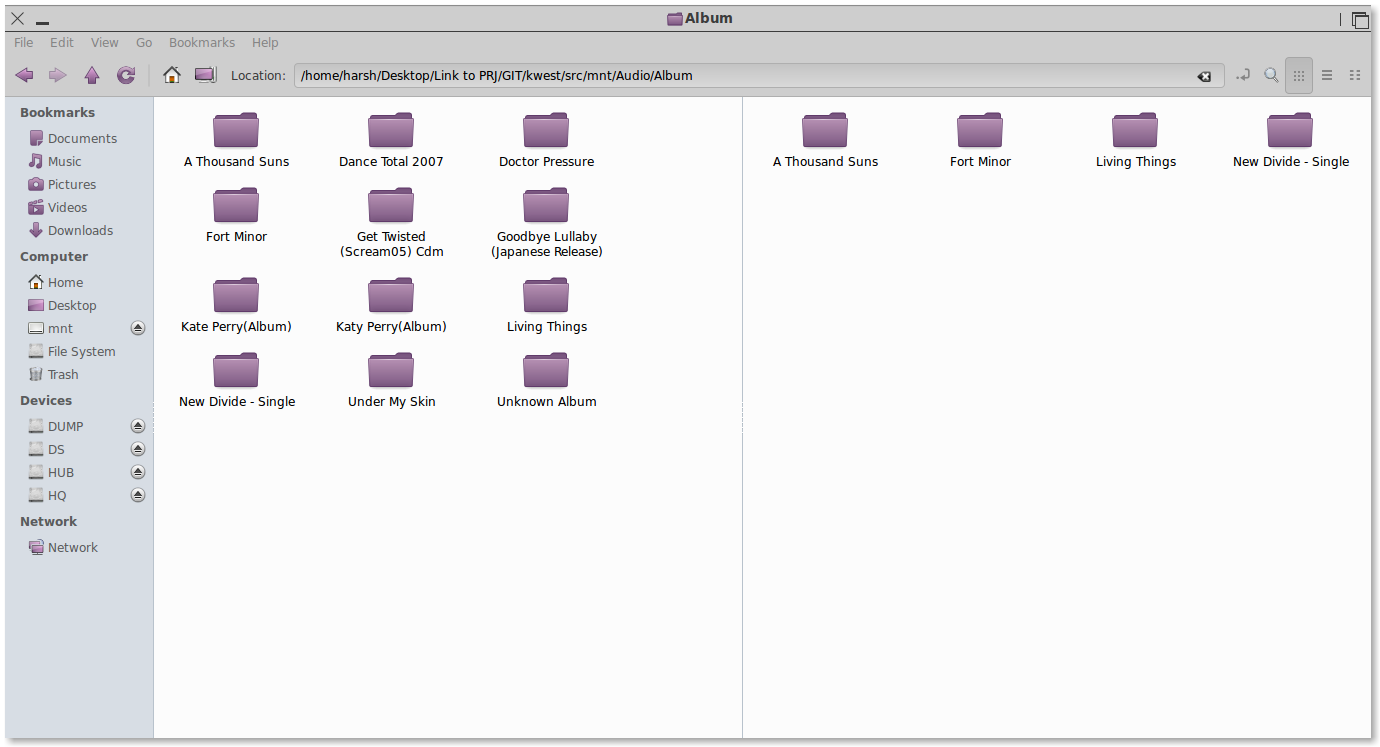
\includegraphics[width=0.8\linewidth]{./opimg/nemo_audiodual.png}}
%\includegraphics[width=0.8\textwidth]{image.png}
\caption{Audio files being categorised by /Album and /Artist/Album views}
\label{fig:dfd0}
\end{figure}

\subsection{Image}
This folder contains all the image files recognised by the system. Inside, the images are organised by ImageCreator and ImageDate. 
The ImageCreator sub folder is based on \textit{Creators} like software - Adobe Photoshop, or hardware - Camera Models. Each ImageCreator tag is further organised by ImageDate. 
The ImageDate folder contains images sorted by \textit{Month-Year} of creation. E.g.: A picture taken on ``\textit{2nd March 1992}'' will appear under ``\textit{1992Mar}''.
As with Audio, files with metadata missing will appear under appropriate \textit{Unknown} sub folders.
\begin{figure}[htb]
\centering
\setlength\fboxsep{0pt}
\setlength\fboxrule{0.5pt}
\fbox{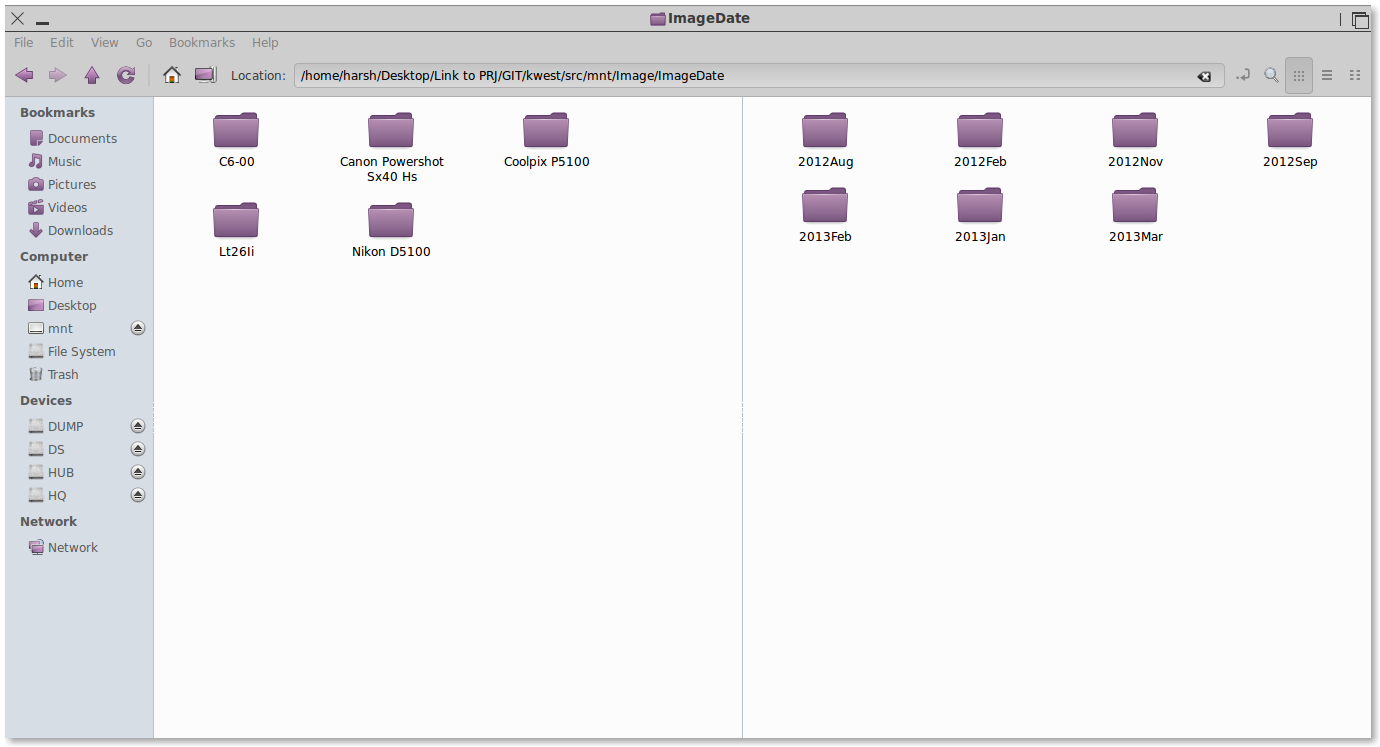
\includegraphics[width=0.8\linewidth]{./opimg/nemo_imagesort.png}}
%\includegraphics[width=0.8\textwidth]{image.png}
\caption{Images being categorised by Creator and CreationDate}
\label{fig:dfd0}
\end{figure}

\subsection{PDF}
All PDF documents are tagged with the PDF tag. Each PDF document is organised by its \textit{Author,Publisher,Subject} and \textit{Title}. Files with metadata missing are appropriately tagged under \textit{Unknown} tags.
\begin{figure}[htb]
\centering
\setlength\fboxsep{0pt}
\setlength\fboxrule{0.5pt}
\fbox{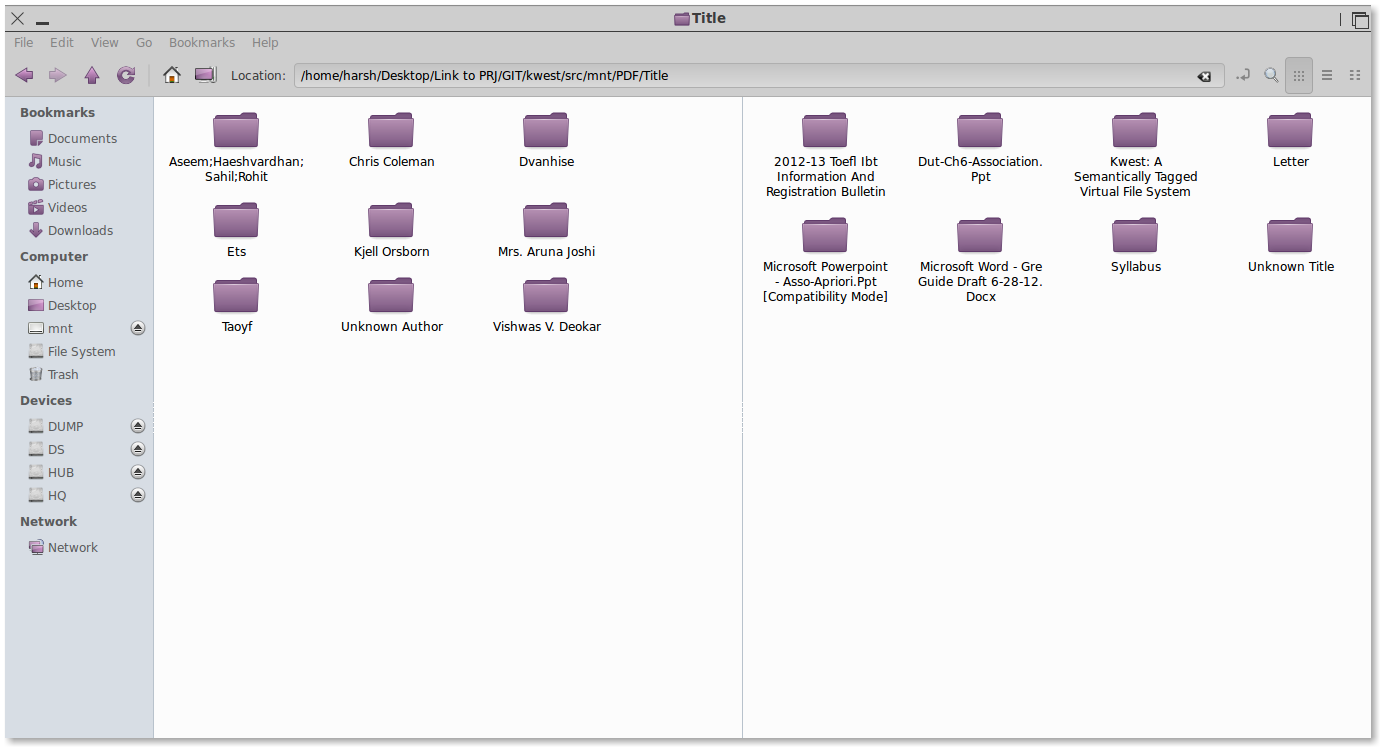
\includegraphics[width=0.8\linewidth]{./opimg/pdfsort.png}}
%\includegraphics[width=0.8\textwidth]{image.png}
\caption{PDF documents being separated by Author and Title}
\label{fig:dfd0}
\end{figure}

\subsection{Video}
Currently, the system organises video based only on Length, with the categories being \textit{Short, Medium and Long}. A short video is anything with less than 1800s of playtime. Videos with play time equal to or greater than 5400s are considered Long, and anything between them is considered Medium. The Video tag does not contain any categories as most of the videos stored by the user do not have any metadata present.
\begin{figure}[htb]
\centering
\setlength\fboxsep{0pt}
\setlength\fboxrule{0.5pt}
\fbox{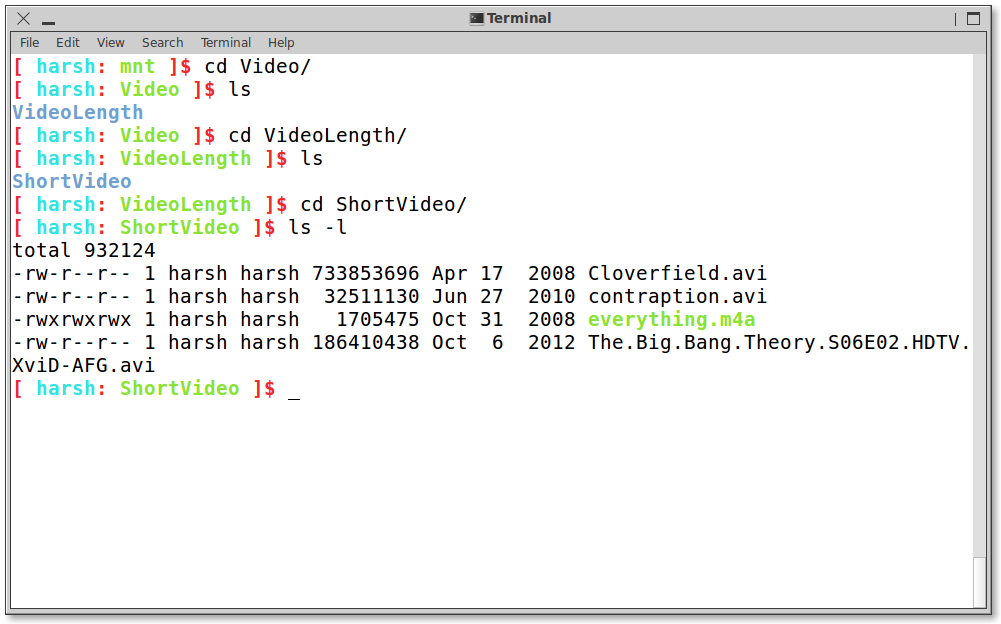
\includegraphics[width=0.8\linewidth]{./opimg/term_video.png}}
%\includegraphics[width=0.8\textwidth]{image.png}
\caption{Browsing the KWEST Video folder in a terminal}
\label{fig:dfd0}
\end{figure}

\subsection{USER}
The tag \textbf{`USER'} refers to the \textit{username} of the current user. The user can create and manage his own personal tags in this folder.
\begin{figure}[htb]
\centering
\setlength\fboxsep{0pt}
\setlength\fboxrule{0.5pt}
\fbox{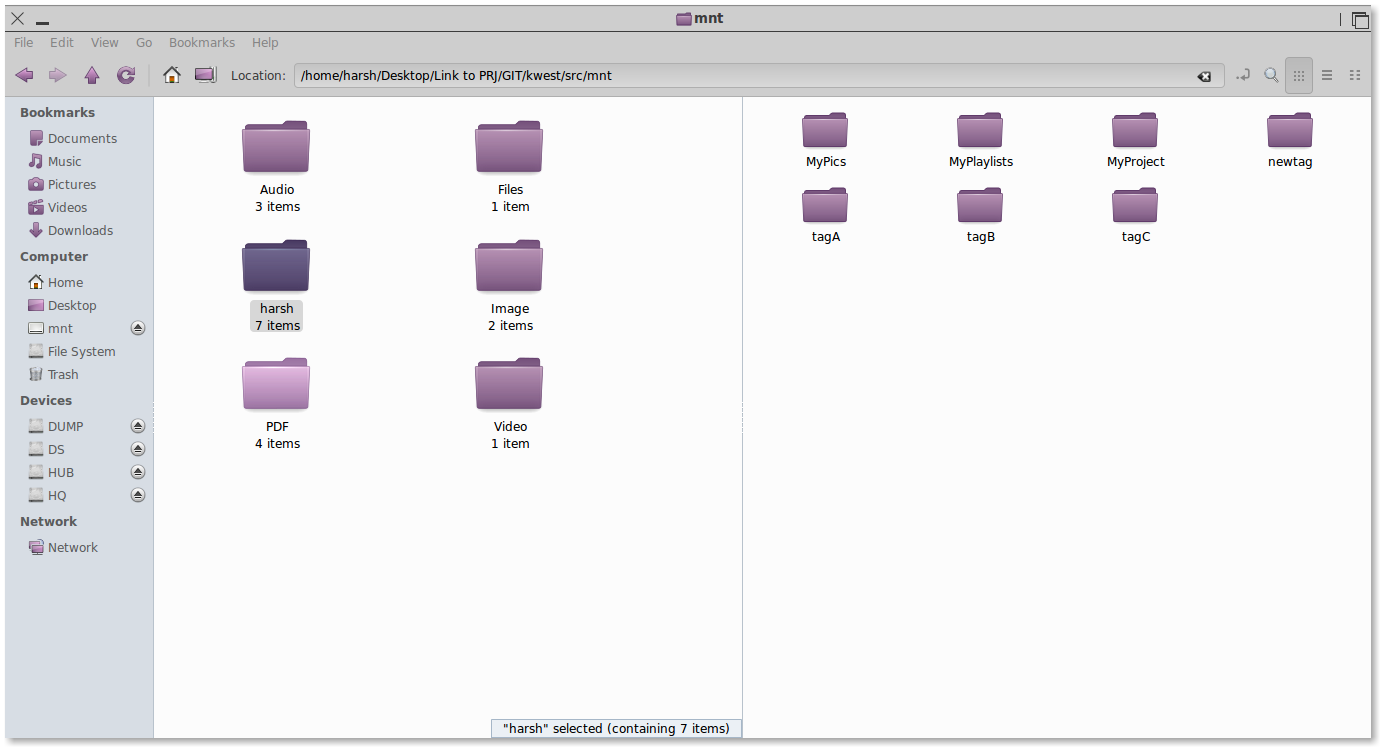
\includegraphics[width=0.8\linewidth]{./opimg/usertags.png}}
%\includegraphics[width=0.8\textwidth]{image.png}
\caption{User tags displayed in KWEST}
\label{fig:dfd0}
\end{figure}


\subsection{Using Suggestions to tag files}
KWEST helps the user with organisation by providing suggestions for tagging files. These suggestions are provided as files prefixed with the word - ``\textit{SUGGESTED}''. The user may make use of that suggestion by tagging that file in the current tag. \newline
e.g. in tag \textit{Zodiac}, there are 3 suggestions: \textit{ARIES, GEMINI, CANCER} each shown as a file with \textit{SUGGESTED} prefixed in their names. To make use of the suggestion on \textit{ARIES}, the user tags the file \textit{ARIES} under the tag \textit{Zodiac}. The file is now seen in the tag without the suggested prefix. The other suggestions are still present and may be used further or deleted.
\begin{figure}[htb]
\centering
\setlength\fboxsep{0pt}
\setlength\fboxrule{0.5pt}
\fbox{\includegraphics[width=0.8\linewidth]{./opimg/suggestions.png}}
%\includegraphics[width=0.8\textwidth]{image.png}
\caption{KWEST offering suggestions for tag favourites}
\label{fig:dfd0}
\end{figure}

%\newpage

\setcounter{section}{0}
\chapter*{DEVELOPERS MANUAL}

\section {KWEST GENERIC API}
The developer can make use of the \textbf{KWEST API} to design and create new plugins for the KWEST file system. Currently, we offer the following API to the user:

\subsection{Database Operations:}
The database KWEST uses is housed in a SQLite repository. Through the use of \textit{database API}, the developer can access the database and perform operations on it. Performing operations directly on the database is not encouraged. Though, if the developers do wish to do so, we provide an API for the same. The database API contains the following headers:
\begin{lstlisting}[language=C,frame=single]
<dbbasic.h> /* basic database operations */
<dbkey.h>   /* key operations for database interaction */
\end{lstlisting}

\subsection{Logfile}
KWEST uses an internal logfile which logs messages in a seperate log file stored in the user's config folder. This logfile is used to print or record error messages and operation statuses while operation. Upon incorrect operations or some system errors, the developer will require the logfile to debug the program. The developer can log to the logfile using the logfile API provided by:
\begin{lstlisting}[language=C,frame=single]
<logging.h> /* log message to logfile */
 /* initialize logging */
int log_init(void); 
 /* print log message to logfile */
void log_msg(const char *msg, ...); 
 /* close the logfile */
int log_close(void);
\end{lstlisting}

\subsection{Data Association rules}
The developer can provide their own suggestions by using a different algorithm or strategy. KWEST uses apriori to form the associations. For the developer to utilise a different approach, he needs to use the \textit{dbapriori.h} file and provide implementations to the defined functions.

\begin{lstlisting}[language=C,frame=single]
/* -------- GENERAL ----------------------- */
int count_user_tags(void);
sqlite3_stmt *get_user_tagname(void);
int add_rule(int type, float c, 
             char *para1, char *para2);
             \end{lstlisting}
\begin{lstlisting}[language=C,frame=single]
/* -------- FILE SUGGESTIONS -------------- */
sqlite3_stmt *get_user_tagged_files(void);
char *get_file_suggestions_pr(char *tagname);
char *get_file_suggestions_r(char *tagname);
/* -------- TAG SUGGESTIONS --------------- */
sqlite3_stmt *get_user_tagged_tags(void);
char *get_tag_suggestions_pr(char *tagname);
char *get_tag_suggestions_r(char *tagname);
/* -------- OTHERS ------------------------ */
void finalize(sqlite3_stmt * stmt);
\end{lstlisting}

\subsection{Flags}
KWEST uses it's own values for flags, stored in a file called as \textit{flags.h}. The developer is encouraged to use the same notations for ease in developing for KWEST. One simply has to include the file to use it.
\begin{lstlisting}[language=C,frame=single]
#include<flags.h> /* KWEST flags and magic numbers */
#define KW_SUCCESS 0 /* return SUCCESS as status */
#define KW_FAIL   -1 /* return FAILED as status */
#define KW_ERROR   1 /* return ERROR as status */

/* FLAGS RELATED TO FUSE, DIRECTORY VALUES */
#define KW_STDIR 0755 /* DIR entry in struct stat */
#define KW_STFIL 0444 /* FILE entry in struct stat */

/* FLAGS RELATED TO DATABASE OPERATIONS */
#define QUERY_SIZE 512 /* Size of array holding query */

#define USER_TAG   1 /* Tag Accessible to user */
#define SYSTEM_TAG 2 /* Tag created and used by system */

/* Starting id for tags and files */
#define NO_DB_ENTRY      -2
#define FILE_START       0
#define SYSTEM_TAG_START 0
#define USER_TAG_START   100
#define USER_MADE_TAG    500

/* Tag-Tag Association Types */
#define ASSOC_PROBABLY_RELATED 1
#define ASSOC_SUBGROUP         2
#define ASSOC_RELATED          3
#define ASSOC_NOT_RELATED      4
\end{lstlisting}

\section{Plugin API}
KWEST provides developers with a \textbf{Plugin API} to help developers create plugins. Each plugin is created by providing implementations for a list of functions defined by KWEST. This is similar to the \textit{OOP} concept of implementing an \textit{interface}. \\
\begin{lstlisting}[language=C,frame=single]
struct plugin_extraction_entry
{
	char *name;
	char *type;
	void *obj;
	bool (*is_of_type)(const char *);
	int (*p_metadata_extract)
		(const char *, struct kw_metadata *);
	int (*p_metadata_update)
		(const char *, struct kw_metadata *);
	int (*on_load)
		(struct plugin_extraction_entry *);
	int (*on_unload)
		(struct plugin_extraction_entry *);
};
\end{lstlisting}

Inside the plugin, the developer may use any library for operations. To create file types, associations with the newly generated metadata, the developer must make use of the \textit{dbplugin.h} API. This API contains the functions to create and manage associations based on the metadata extracted from a file.

\begin{lstlisting}[language=C,frame=single]
 /* Add new mime type to Kwest */
void add_mime_type(char *mime);
 /* Add new metadata type to existing mime type */
void add_metadata_type(char *mime, char *metadata);
 /* Form association for metadata in file */
void associate_file_metadata(const char *mime,
		const char *tagname,const char *fname);
 /* Form association between tags */
void associate_tag_metadata(const char *mime,
       const char *tagname,const char *parentmime,const char *parent);
\end{lstlisting}

\section{Extracting metadata}
When the developer writes a new plugin for some file type, the plugin must implement the  function \textit{metadata\_ extract} which will return a metadata structure containing the file's associated metadata. This structure is defined in the file \textit{metadata\_ extract.h}
\begin{lstlisting}[language=C,frame=single]
struct kw_metadata {
	/** type of metadata */
	char  *type; 
	\end{lstlisting}
\begin{lstlisting}[language=C,frame=single]
	/** number of tags in metadata */
	int tagc; 
	/** tag type array */
	char **tagtype; 
	/** tag value array */
	char **tagv; 
	/** object for use by plugin */
	void *obj; 
	/** initialization options upon extraction */
	int (*do_init)(void *); 
	/** callback function for cleaning up metadata */
	int (*do_cleanup)(struct kw_metadata *); 
};
\end{lstlisting}

\section{Debugging}
The KWEST file system utilises the fuse kernel module for creating a virtual file system. Debugging a KWEST program is a little bit complex as it cannot be traced using normal debug calls. For debugging you can use the following tools:
\subsection*{GDB - GNU Project Debugger}
The GDB can debug a KWEST file system in single process foreground mode. To debug using GDB, do:
\begin{lstlisting}[language=bash,frame=single]
gdb program_name
run -d -s -f <mount_directory>
\end{lstlisting}
The GDB will execute the program and mount the file system. The developer can use the file system in another terminal or browser, this instance of GDB needs to be in action for the developer to debug the program. In case of an error or interrup, GDB will display error messages accordingly. The developer can further view the error calls using:
\begin{lstlisting}[language=bash,frame=single]
stack bt
stack ft
\end{lstlisting}

\subsection*{Valgrind}
Valgrind is an industry level tool which helps find errors and memory leaks in the program. To run a fuse file system like KWEST under Valgrind, the developer can issue the following command:
\begin{lstlisting}[language=bash,frame=single]
valgrind --tool=memcheck --trace-children=no 
         --leak-check=full --track-origins=yes -v 
         ./program_name mount_point -d -f -s
\end{lstlisting}

\section{F.A.Q.}
\begin{enumerate} 
\item \emph{The project won't compile. I followed the steps correctly, but there are some errors while building...} \newline
Make sure you have all the dependencies installed and they are up-to-date with the requirments. Sometimes, a system error may interfere in the installation, you may want to restart and try again. The installation does not require administrative privelages, however, you must be able to execute the make file for the installation.
\item \emph{It gives some error regarding missing kw libraries. Where do I get them?} \newline
This is due to the libraries being incorrectly linked. You can retype the \textit{export} command from the installation steps.
\item \emph{I get compile time errors on the KWEST API} \newline
Every KWEST API feature has been thoroughly tested before recommendation. KWEST itself internally uses this API to manage it's plugin. Make sure you have properly cross-compiled the libraries and have included proper header files and try again.
\item \emph{I get \texttt{segmentation fault} errors and the program crashes.} \newline
This happens mostly due to file system corruption. You can try unmounting and mounting the file system again. If this still does not solve the issue, you may have to re-install or compile the program.
\item \emph{The extraction library I want to use is not available in C} \newline
All you need to use a library in your language is a C API for that libary function. As long as the developer can gurantee that the library and it's associated operations will execute on the target machine, KWEST can run the plugin with external dependencies.
\item \emph{Where do I get documented API for KWEST?} \newline
The KWEST source code is documented using the doxygen documentation system. The source code contains a \textit{doxygen} file which can be compiled to produce Doxygen files which will provide the documentation.
\item \emph{What if I want to change a file system operation behaviour?} \newline
Sorry, we do not provide an API to do that. However, since KWEST itself is open source, you can change the operations freely.
\end{enumerate}
\chapter{Conclusion and Future Scope}

\section{Conclusion}

\subsection*{Considering data organisation}
A file system, considering that it stores data, is created with stability and performance in mind. An end-user is more concerned with how they can store and access their data efficiently. Using a KWEST file system, the user can organise their data efficiently. All files are stored and accessed by their content or context rather than just a bunch of string-names. This allows the user to think and remember the file in terms of what it represents, rather than a path-name which may not be related to the data it contains. This semantic approach is helpful to the user, as it becomes easier to manage for them to search for and manage their data.

\subsection*{Automation of tasks}
KWEST automatically uses the metadata embedded in a file to apply tags and categorise it. This automation helps the user by providing access to files according to their respective contexts. By doing this, the user gets all Audio files under the \textit{Audio} folder, all Image files under the \textit{Image} folder and so on. Further, each folder is organised by meta-type belonging to that mime type. E.g. the \textit{Audio} folder is sorted by \textit{Album, Artist, Genre}.

\subsection*{Providing suggestions}
It may happen that the user inadvertently misses out tagging some file, which may result in an incomplete organisation. The user may later search for that particular file in the tag, but will not find it. In a KWEST file system, based on the occurrences of files in various user tags, the system provides \textit{suggestions} that help the user tag a file in appropriate places. This helps avoid missing out on important files, and allows a faster method of organisation as the files to be tagged are available as suggestions.

\subsection*{Performance and stability}
Although a KWEST file system is created and operates as a VFS, there is no perceptible lag or performance hit on the operations the user performs. Common operations like listening to music, watching a video, writing to a document can be carried out smoothly.

Also, since KWEST is based on an always stable implementation of FUSE, the file system itself is stable. Strict coding standards and rigorous tests against memory allow the file system to remain stable even under moderate usage.


\section{Future Scope}

The project, with its novel concept of \textit{Applying association rule learning in a semantic file system}; is the first implementation of a semantic file system to actively help the user categorise and organise their data.

\subsection*{Support for more standard file types}
Right now the import feature can extract metadata only from a fixed set of file types. More file types can be handled which increase the feature and usefulness of the file system. Every operating system or file manager has a certain knowledge of what kind of metadata each file type can contain. Using this knowledge in the KWEST file system will allow the user to be able to browse a file system completely based on it's semantics.

\subsection*{More relations and associations}
Currently, the system creates associations based on the common occurrences of files between various tags. This is done using the Apriori algorithm. There are a lot of other interesting approaches which can be utilised. Like algorithms to create various different associations. Or changing the way Apriori handles files and tags. File accesses, frequency of usage, explicit user choices can also be utilised for forming results.

\subsection*{Efficiency and Performance}
Although the system is both efficient and performant, it can be vastly improved to provide a high-quality file system. Operations can be threaded to reduce the wait time. Simultaneous access to files can be used to provide a fluid experience. Algorithm throughput can be raised to get more accurate results. These are just a few performance and efficiency related things we can do with KWEST. The ultimate approach is to integrate this file system at the kernel level. This will allow performance and stability similar those of traditional file systems.

\subsection*{Collect data from various locations}
The KWEST file system imports data only from the user's \textit{HOME} folder. The data stored there might not be the only location a user wants to use. In today's world, each person has a multitude of devices ranging from laptops, PCs, tablets and phones to Cloud services like Dropbox, Google Drive. Each of them have data which the KWEST file system can utilise to form associations and display using virtual suggestions. It will result in a unified view of all the user's data categorised and organised, which is spread and available across all of their devices.

\section{Need for KWEST tomorrow}
With data usage almost doubling with each passing year, people are bound to focus on organising it. A tool like KWEST,  with its semantic roots, automation and suggestions will be immensely helpful when a large data storage has to be properly catalogued, organised and accessed. Thus, we have tried to implement a research based project with its usefulness reflected in the problems of tomorrow.
\renewcommand{\thesection}{\Alph{section}} 
\chapter{APPENDIX}
%\setcounter{section}{A}
\begingroup
\let\clearpage\relax
\phantomsection
\addcontentsline{toc}{section}{\protect\numberline{}\textbf{Appendix A:} Mathematical Model}%
\chapter*{A: MATHEMATICAL MODEL}
\endgroup
The relationship between files and tags can be represented by using Set theory. Set theory is the branch of mathematics that studies sets, which are collections of objects. The following mathematical model represents the working of this filesystem. 

\noindent The following dynamic and variable sets are defined as, \\
\indent $F$	: Set of Files \\
\indent $T$	: Set of Tags \\
\indent $S$	: Set of Tags in query ( $S \subseteq T$ ) \\

\subsection{Relation between Files (F) and Tags (T)}
$$ R = \{(f,t) \mid f \,\, has \,\, tag \,\,t; f \in F, t \in T\}$$
Here $R$ defines the relation between a file $f$ and its tag $t$ where $R \subseteq F \times T$. This relationship is \emph{many-to-many}. 
That is a file can have many tags, and a tag can describe many files.

\subsection{Association between Tags (T)}
Using discovered associations, we can form various relations between tags. These \emph{tag-to-tag} help in displaying related information. For any two tags there exists a distinct relation between them given by $r$. The function $X_{r}(A,B)$ returns the relation between two tags. Associations can be broadly categorized as:
\begin{itemize}
\item {$A \sim B$} : $A$ and $B$ are not directly related, but there \emph{may} exist some indirect relation between them.
\item $A \succ B$ : $A$ and $B$ are directly related, where $A$ always has a path leading to $B$. This relation is similar to $A \subset B$.
\item $A \bowtie B$ : $A$ and $B$ are not directly related, but $B$ supplements additional information related to $A$.
\item $\phi$ : This relation states that there does not exist any relation between the two tags.
\end{itemize}

\subsection{Operations}
$$g(f) = \{t : f \, R \, t\}$$
$g$ is an operation which takes input as a file $f$ and returns the set of tags ($t \in S$) related by $R$ to that file.

$$h(t) = \{f : f \, R \, t\}$$
$h$ is an operation which takes input as a tag $t$ and returns the set of files ($f \in F_{S}$) related by $R$ to that tag.

%----------------------------------------------------------------------------------------------------------------------------------

\subsection{Storing Tags and Files}
The relation $R$ is stored as a set of ordered pairs $(f,t)$, where $R \subseteq F \times T$. The operations $g$ and $h$ operate on these ordered pairs and return mapped or matched elements. A relation which has to be added must be represented in the form of of ordered pair $(f,t)$. Storage of all relations is given by $F \times T$ where ordered pairs exist according to $R = \{f \in F, t \in T \mid f\, R \,t\}$.

\noindent For example, we have the sets and their relations as: 
$$F = \{ f_{1}, f_{2}, f_{3} \}, T = \{ t_{1}, t_{2}, t_{3} \}, R = \{f_{1} \, R  \, t_{1}, f_{2}  \, R  \, t_{2}, f_{3}  \, R  \, t_{1}, f_{1}  \, R  \, t_{3}\}$$
Then we store this relation by its ordered pairs given by:
$$R = \{(f_{1},t_{1}),(f_{2}, t_{2}),(f_{3}, t_{1}),(f_{1}, t_{3})\}$$

\subsection{Extraction of metadata}
The extraction of metadata is defined by the function $X_{E}$ which takes a file $f(f \in F)$ and returns a set of tags $(T_{E} \subseteq T)$ that form the relation ($f  \, R  \, t : t \in T_{E}$). 
$$X_{E}(f) = T_{E} \in 2^{T}$$

\noindent Addition of new information (metadata, tags) is done as:
$${if (t \notin T) \, then \, (T \gets T \cup \{t\})}$$

\noindent We then store this relation as a ordered pair $\{(f, \, t) \, \forall t \in T_{E}\}$. At the end of this operation $T_{E} \subseteq T$ will hold true. 

\subsection{Importing Semantics}
The existing file-directory structure can be imported to the system and represented in the form of tags and files. We define: 

\noindent $F_{H} \, $  : Set of \emph{Files} on hard-disk which are not represented in system.\\
$D_{H}$ : Set of \emph{Directories} on hard-disk which are not represented in system. \\

\noindent Then for every file stored within a directory $d$, the relation $R$ is expressed as 
$(f  \, R  \, d)$.
When importing semantics we create the ordered pair $(f,d)$ given by the relation $(f  \, R \,  d, \forall d \in D_{d})$. Where $D_{d}$ contains the directory the file is stored in, as well as every parent directory of that directory itself.

\noindent Directories also contain sub-directories which we store in the form of tag relationships. We represent them as:
$\forall (d_{1}, d_{2}) \in D_{H}$, if $d_{2} \subset d_{1}$ ($d_{2}$ is a sub-directory of $d_{1}$) store the relation as
$$d_{1} \to d_{2}$$


\subsection{Apriori Algorithm}
The apriori algorithm\cite{FastAlgo} is a classic algorithm for learning association rules. The
 algorithm is designed to operate on databases containing transactions. As is
common in association rule mining, given a set of itemsets (for instance, sets
of retail transactions, each listing individual items purchased), the algorithm
attempts to find subsets which are common to at least a minimum number C of the
itemsets. Apriori uses a "bottom up" approach, where frequent subsets are
extended one item at a time (a step known as candidate generation), and groups
of candidates are tested against the data. The algorithm terminates when no
further successful extensions are found.

The purpose of the apriori algorithm is to find associations between different sets of data.
Each set of data has a number of items and is called a transaction.
The output of Apriori is sets of rules that tell us how often items are contained in sets of data.

\subsubsection{Itemset}
A collection of one or more items. \\
Example: {A, B, C} \\ \\
\textbf{k-itemset} \\
An itemset that contains k items.

\subsubsection{Support count (S)}
Number of transactions containing an itemset. \\
Example: S({A, B}) = 2

\subsubsection{Support (supp)}
The support supp(X) of an itemset X is defined as the proportion of transactions in the data set which contain the itemset.
Suppose \textit{minsup} is the minimum support threshold.
Example: supp({A, B}) = 2/5

\subsubsection{Frequent Itemset (L)}
An itemset satisfies minimum support if the occurrence frequency of the itemset
is greater or equal to a threshold. If an itemset satisfies minimum support, then it is a frequent itemset.
Thus an itemset whose support is greater or equal to minsup is a frequent itemset.

\subsubsection{Confidence}
The confidence of a rule is defined as,\\
\begin{equation}
Conf(A \rightarrow B) = supp(A \rightarrow  B) / supp(A)
\end{equation}
Suppose \textit{minconf} is the minimum confidence threshold.

\subsubsection{Rule Generation}
Given a set of transactions T, the goal of association rule mining is to find all rules having\\
\begin{equation}
support \geq minsup \; threshold
\end{equation}
\begin{equation}
confidence \geq minconf \; threshold
\end{equation}

Given a frequent itemset L, find all non-empty subsets $f \subset L$ such that $f \rightarrow  L - f$ satisfies the minimum confidence requirement.

Example: If ${A, B, C}$ is a frequent itemset, then the following candidate rules are formed \\
${ AB \rightarrow  C, \; AC \rightarrow  B, \; BC \rightarrow  A, \; A \rightarrow  BC, \; B \rightarrow  AC, \; C \rightarrow  AB }$ 

If $|L| = k$, then there are $(2 ^ k) - 2$ candidate association rules 
$(ignoring \,\; L \rightarrow \Phi \; and \;\; \Phi \rightarrow L)$

\subsubsection{Apriori principle}
The princciple sttes that if an itemset is frequent, then all of its subsets must also be frequent.
Apriori principle holds due to the following property of the support measure:
\begin{equation}
\forall X , Y : ( X \subseteq Y ) \rightarrow  s( X ) \geq s(Y )
\end{equation}

Support of an itemset never exceeds the support of its subsets. This is known as the anti-monotone property of support.

$\newline$
\textbf{Algorithm} \\
Input \\
T - Database of transactions \\
I   - Items \\
L - Itemset\\
s   - support\\
c - confidence

$\newline$
Output \\
R - Association rules satisfying s and c

$\newline$
Algorithm to Generate Frequent Itemsets\\
Apriori(T,s)\\
$L_{1} \leftarrow {Large \; 1-itemset} \\
k \leftarrow 2 \\
while \; L_{k - 1} \neq \Phi \\
C_{k} = Generate(L_{k - 1}) \\
	for \;  transactions  t \in T \\
		C_{t} \leftarrow Subset(C_{k}, t) \\
		for \; candidates \; c \in C_{t} \\
			count[c] \leftarrow \; count[c] + 1 \\
		L_{k} \leftarrow {c \in C_{k} | count[c] \geq s} \\
		k \leftarrow k + 1 \\
return \cup L_{k}$

$\newline$
Algorithm to Generate Association Rules\\
GenRule\\
$R = \Phi;\\
	for \; each \; l \in L \; do \\
		for \; each \; x \subset l \; such \; that \; x \neq \Phi \; and \; x \neq l \; do \\ 
			if (supp(l) \; / \; supp(x)) \geq c \; then \\
				R = R \; \cup \; ( x \rightarrow ( l - x ) )$;
				
				
				
\newpage				
\setcounter{subsection}{1}
\setcounter{subsubsection}{1}
\phantomsection
\addcontentsline{toc}{section}{\protect\numberline{}\textbf{Appendix B:} Testing of Data}
\chapter*{B: TESTING OF DATA}

Testing of the system will be done on the following points:

\subsection{Storing the relation $R$:}
The working of the system depends on correctly storing the relation $R$. These tests check whether the relations are stored and represented correctly. 
\begin{enumerate}
\item For any file $f$ associated with tag $t$ there should exist an ordered pair $(f,t)$.
\item For a file $f$ associated with tags $S = \{t_{1}, t_{2}, t_{3}\}$, the operation $g(f)$ should return exacty $S$.
\item For a tag $t$ containing files $F = \{f_{1}, f_{2}, f_{3}\}$, the operation $h(t)$ should return exactly $F$.
\end{enumerate}

\subsection{Relation between tags: }
\begin{enumerate}
\item The relation $r$ between two tags $t_{1},t_{2}$ is given by function $X_{r}(t_{1},t_{2})=c$.
\item The relation $r$ is distinct i.e. there exists only one relation between any two tags. If contradictions arise where more than one relation is present between two tags, then all those relations must be made void and $r=\phi$. The user can then explicitly specify which relation should be created between those two tags.
\item Extensive testing must be done on relations to determine which $r$ needs to be set under certain conditions.
\end{enumerate}

\subsection{Extraction of Metadata:}
Let $M$ be the set of all metadata tags $t$ for file $f$. The function $X_{E}$ represents an algorithm to extract t from f. It returns a set $T_{E}$ such that $\{t \in T_{E} \mid f \, R \, t\}$ and $(T_E \subseteq M)$. To test the efficiency of the function, or the effectiveness of it, we compare the cardinality of the generated set $T_E$ with the set of Metadata $M$. The efficiency can be calculated by
$$\mathrm{Efficiency} \, \epsilon = \frac {\mid T_E \mid} {\mid M \mid}$$
Using $\epsilon$ we can compare algorithms and their efficiency. Appropriate algorithms can be chosen for various file types so that efficiency of the entire system remains high. For e.g. \\
\indent $X_{E1} : \{\epsilon =0.7$ for audio$, \epsilon = 0.4$ for images $\}$ \\
\indent $X_{E2} : \{\epsilon =0.6$ for audio$, \epsilon = 0.6$ for images $\}$ \\
Then we have the following options:
\begin{enumerate}
\item $X_{E2}$ is a better choice as it yeilds a more consisten efficiency.
\item $X_{E1}$ is used only for audio and $X_{E2}$ is used only for image extractions.
\end{enumerate}


\subsection{Queries and their results:}
Queries are parsed into tokens of the form $(t_1, \sigma , t_2)$. We need to test whether $\sigma $ returns the correct results for the query. A Query $Q(S)$ is said to be successfully executed when the expected result are shown.  
\begin{itemize}
\item The Query $q(t)$ for a single tag $t$ should return a set of files $(f \in F_{S})$ through the operation $h(t)$. 
\item In a query if no operation is given, Intersubsection should be performed. 
\item For Query $Q(S)$ the operations should be performed from left to right unless precedence is specified by paranthesis. 
\end{itemize}

Example:
\noindent Let $t_{1}, t_{2}, t_{3}$ be tags having the following files: \\
\indent $t_{1}$ : $\{photo_{1},photo_{2},doc_{1}\}$  \\
\indent $t_{2}$ : $\{photo_{1},doc_{1}, ppt_{1}\}$  \\
\indent $t_{3}$ : $\{photo_{1},doc_{3}\}$ 
\begin{enumerate}
\item $q(t) = F_{S}$ where $f$ should follow the relation $(f \in F_S \mid f \, R \, T)$. 
For example, q$(t_{1})$ returns $F_S = \{photo_{1},photo_{2},doc_{1}\}$.
\item Consider a query containing tags $S = \{t_{1}, t_{2}\}$. 
It generates results by performing the operations $Q(S) = q(t_{1})\sigma q(t_{2})$
where $\sigma $ is an operator.
\begin{enumerate}
\item Putting $\sigma = \cup$ for Union in query $Q(S) = q(t_{1})\cup q(t_{2})$; the result should be $F_S = \{photo_1, photo_2, doc_1, ppt_1\}$. 	
\item Putting $\sigma = \cap$ for Intersubsection in query $Q(S) = q(t_{1})\cap q(t_{2})$; the result should be $F_S = \{photo_1, doc_1\}$.
\item Putting $\sigma = \setminus$ for Set Difference in query $Q(S) = q(t_{1})\setminus q(t_{2})$; the result should be $F_S = \{photo_2\}$, whereas the query $Q(S) = q(t_{2}) \setminus q(t_{1})$ will return the result as $F_S = \{ppt_1\}$.
\item Putting $\sigma = \ominus$ for Symmetric Difference in query $Q(S) = q(t_{1})\ominus q(t_{2})$; the result should be $F_S = \{photo_2, ppt_1\}$.
\end{enumerate}

\item Consider a query containing tags $S = \{t_{1}, t_{2}, t_{3}\}$.
It performs operations as : $Q(S) = q(t_{1})\sigma_{1} q(t_{2})\sigma_{2} q(t_{3})$
The default order for processing is from left to right unless precedence is specified through parenthesis.

\begin{enumerate}
\item For the query $Q(S) = q(t_{1}) q(t_{2}) q(t_{3})$ the result will be returned as files $\{photo_{1}\}$
\item For the query $Q(S) = q(t_{1}) \cup q(t_{2}) \cap q(t_{3})$ the result will be returned as files $\{photo_{1}, doc_{1}, doc_{3}\}$
\end{enumerate}
\end{enumerate}

After verifying that individual queries return correct results, we must check whether $Q(S)$ runs correctly as well. This is done by seperating the query into tokens, and calculating their results in turn. It must be verified that results are correct and have not been mis-intepreted through tokenization of the query.
%----------------------------------------------------------------------------------------------------------------------------------------

\subsection{Forming Associations}
Consider a database, D, consisting of 9 transactions.
Suppose minimum support count required is 2 (i.e. $minsup = 2 / 9 = 22\%$ ).
Let minimum confidence required is $minconf = 70\%$.
We have to first find out the frequent itemset using apriori algorithm.
Then, Association rules will be generated using minsup and minconf.

\begin{center}
\begin{tabular}{|l|l|}
\hline
\textbf {TagID} & \textbf {Files} \\ \hline
T100 & F1, F2, F5  \\ \hline
T101 & F1, F2, F5  \\ \hline
T102 & F2, F4  \\ \hline
T103 & F2, F3  \\ \hline
T104 & F1, F2, F4  \\ \hline
T105 & F1, F3  \\ \hline
T106 & F2, F3  \\ \hline
T107 & F1, F3  \\ \hline
T108 & F1, F2, F3, F5  \\ \hline
T109 & F1, F2, F3  \\ \hline
\end{tabular}
\end{center}

$\newline$
\textbf{Step 1: Generating initial Candidate Itemset} \\
In the first iteration of the algorithm, each item is a member of the set of candidate.

\begin{center}
\begin{tabular}{|l|l|}
\hline
\textbf {Itemset} & \textbf {Support count} \\ \hline
\{F1\} & 6  \\ \hline
\{F2\} & 7  \\ \hline
\{F3\} & 6  \\ \hline
\{F4\} & 2  \\ \hline
\{F5\} & 2  \\ \hline
\end{tabular}
\end{center}

$\newline$
\textbf{Step 2: Generating 1-itemset Frequent Pattern} \\
The set of frequent 1-itemsets, L1, consists of the candidate 1-itemsets satisfying minimum support.

\begin{center}
\begin{tabular}{|l|l|}
\hline
\textbf {Itemset} & \textbf {Support count} \\ \hline
\{F1\} & 6  \\ \hline
\{F2\} & 7  \\ \hline
\{F3\} & 6  \\ \hline
\{F4\} & 2  \\ \hline
\{F5\} & 2  \\ \hline
\end{tabular}
\end{center}

$\newline$
\textbf{Step 3: Generating 2-itemset Frequent Pattern} \\
To discover the set of frequent 2-itemsets, L2, the algorithm uses L1 Join L1 to generate a candidate set of 2-itemsets, C2.
Next, the transactions in D are scanned and the support count for each candidate itemset in C2 is accumulated.
The set of frequent 2-itemsets, L2, is then determined, consisting of those candidate 2-itemsets in C2 having minimum support.

\begin{center}
\begin{tabular}{|l|l|}
\hline
\textbf {Itemset} & \textbf {Support count} \\ \hline
\{F1, F2\} & 4  \\ \hline
\{F1, F3\} & 4  \\ \hline
\{F1, F5\} & 2  \\ \hline
\{F2, F3\} & 4  \\ \hline
\{F2, F4\} & 2  \\ \hline
\{F2, F5\} & 2  \\ \hline
\end{tabular}
\end{center}

$\newline$
\textbf{Step 4: Generating 3-itemset Frequent Pattern}\\
The generation of the set of candidate 3-itemsets, C3, involves use of the Apriori Property. First, we generate C3 using L2 join L2. \\
\begin{center}
C3 = \{\{F1, F2, F3\}, \{F1, F2, F5\}, \{F1, F3, F5\}, \\
\{F2, F3, F4\}, \{F2, F3, F5\}, \{F2, F4, F5\}\}.
\end{center}
Now we will apply Apriori property to determine which candidate itemsets are frequent.

The 2-item subsets of \{F1, F2, F3\} are \{F1, F2\}, \{F1, F3\} and \{F2, F3\}.
Since all 2-item subsets of \{F1, F2, F3\} are members of L2, We will keep \{F1, F2, F3\} in C3.

The 2-item subsets of \{F2, F3, F5\} are \{F2, F3\}, \{F2, F5\} and \{F3, F5\}.
But, \{F3, F5\} is not a member of L2 and hence it is violating Apriori Property.
Thus we will remove \{F2, F3, F5\} from C3.
Therefore,
\begin{center}
C3 = \{\{F1, F2, F3\}, \{F1, F2, F5\}\}.
\end{center}
Now, the transactions in D are scanned in order to determine L3, consisting
of those candidates 3-itemsets in C3 having minimum support.

\begin{center}
\begin{tabular}{|l|l|}
\hline
\textbf {Itemset} & \textbf {Support count} \\ \hline
\{F1, F2, F3\} & 2  \\ \hline
\{F1, F2, F5\} & 2  \\ \hline
\end{tabular}
\end{center}

$\newline$
\textbf{Step 5: Generating 4-itemset Frequent Pattern}\\
The algorithm uses L3 Join L3 to generate a candidate set of 4-itemsets, C4.
Although the join results in \{\{F1, F2, F3, F5\}\}, this itemset is removed since its subset \{\{F2, F3, F5\}\} is not frequent.
Thus, $ C4 = \Phi $ , and algorithm terminates, having found all of the frequent items.
This completes our apriori algorithm.

$\newline$
\textbf{Step 6: Generating Association Rules from Frequent Itemsets} \\
For each frequent itemset 'l', generate all nonempty subsets of l.
For every nonempty subset s of l, output the rule $ s \rightarrow  (l-s) $ if $ supp(l) \; / \; supp(s) \geq minconf $

We had L = \{\{F1\}, \{F2\}, \{F3\}, \{F4\}, \{F5\}, \{F1, F2\}, \{F1, F3\}, \{F1, F5\}, \{F2, F3\}, \{F2, F4\}, \{F2, F5\}, \{F1, F2, F3\}, \{F1, F2, F5\}\}.

Consider l = \{F1, F2, F5\}. Its all nonempty subsets are \{F1, F2\}, \{F1, F5\}, \{F2, F5\}, \{F1\}, \{F2\}, \{F5\}.

The association rules are shown below, each listed with its confidence.
\begin{enumerate}
\item $R1: F1, F2 \rightarrow F5 \\
Confidence = supp\{F1, F2, F5\} / supp\{F1, F2\} = 2 / 4 = 50 \% $ \\
R1 is Rejected.
\item $R2: F1, F5 \rightarrow F2$\\
$Confidence = supp\{F1, F2, F5\} / supp\{F1, F5\} = 2 / 2 = 100 \% $\\
R2 is Selected.
\item $R3: F2, F5 \rightarrow F1$\\
$Confidence = supp\{F1, F2, F5\} / supp\{F2, F5\} = 2 / 2 = 100 \% $\\
R3 is Selected.
\item $R4: F1 \rightarrow F2, F5$\\
$Confidence = supp\{F1, F2, F5\} / supp\{F1\} = 2 / 6 = 33 \% $\\
R4 is Rejected.
\item $R5: F2 \rightarrow F1, F5$\\
$Confidence = supp\{F1, F2, F5\} / supp\{F2\} = 2 / 7 = 29 \% $\\
R5 is Rejected.
\item $R6: F5 \rightarrow F1, F2$\\
$Confidence = supp\{F1, F2, F5\} / supp\{F5\} = 2 / 2 = 100 \% $\\
R6 is Selected.
\end{enumerate}

In this way, we have found the following three strong association rules.
\begin{enumerate}
\item $F1, F5 \rightarrow  F2$
\item $F2, F5 \rightarrow  F1$
\item $F5 \rightarrow  F1, F2$
\end{enumerate}

%\newpage
%\input{testingofdata.tex}
\newpage
%\setcounter{section}{A}
\setcounter{subsection}{1}
\setcounter{subsubsection}{1}
\phantomsection
\addcontentsline{toc}{section}{\protect\numberline{}\textbf{Appendix C:} Papers Published}
\chapter*{C: PAPERS PUBLISHED}

%\begin{table}[h]
\begin{center}
\begin{tabular}{p{1cm}p{12cm}}

\textbf{Sr.No.} & \textbf{Paper Name} \\ 

$[1]$ & A. Gogte, S. Gupta, H. Pandit, R. Sharma, \textit{Using association rule learning in a Semantic file system}, International Conference on Advanced Computer Sciences and Information Technology, Pune, Februrary 15, 2013, 
pp. 29-31. $[\textbf{Published}]$\\

$[2]$ & A. Gogte, S. Gupta, H. Pandit, R. Sharma, \textit{KWEST - A Semantically Tagged Virtual File System}, International Conference on Advanced Computer Engineering and Applications, Trivandrum, 2012. $[Accepted]$\\

\end{tabular}
%\caption{Paper Published}
\end{center}
%\label{tag:PP}
%\end{table}

\subsection*{1.}
\includegraphics[page=1,scale=0.35]{./appendix/paperpage1.pdf}
\includepdf[scale=0.85,pages=1-,offset=20 10,pagecommand={}]{./appendix/paperpage2.pdf}	
\includepdf[scale=0.85,pages=1-,offset=20 10,pagecommand={}]{./appendix/paperpage3.pdf}	

%\hspace*{-1.5cm}
\subsubsection{Reviewers comments:}
\begin{figure}[!h]
\centering
\setlength\fboxsep{0pt}
\setlength\fboxrule{0.5pt}
\fbox{\includegraphics[width=0.8\linewidth]{./appendix/paper2review.jpg}}
%\includegraphics[width=0.8\textwidth]{image.png}
\caption{Reviewers comments}
\label{fig:RC1}
\end{figure}

\newpage
\subsection*{2.}

\includegraphics[page=1,scale=0.75]
{./appendix/sem1.pdf}
\includepdf[scale=0.85,pages=2-,offset=20 10,pagecommand={}]{./appendix/sem1.pdf}

\subsubsection{Reviewers comments:}
\begin{figure}[!h]
\centering
\setlength\fboxsep{0pt}
\setlength\fboxrule{0.5pt}
\fbox{\includegraphics[width=0.8\linewidth]{./appendix/paper1review.png}}
%\includegraphics[width=0.8\textwidth]{image.png}
\caption{Reviewers comments}
\label{fig:RC2}
\end{figure}

\newpage
%\setcounter{section}{A}
\setcounter{subsection}{1}
\setcounter{subsubsection}{1}
\section*{APPENDIX D: PAPERS REFERRED}

\section{KFS - KNOWLEDGE FILE SYSTEM}
\hspace*{-1.5cm}
\includegraphics[page=1,scale=0.75]{./appendix/KFS.pdf}
\includepdf[scale=0.85,pages=2-,offset=20 10,pagecommand={}]{./appendix/KFS.pdf}


\section{Semantic-Aware Metadata Organization Paradigm in Next-Generation File Systems}
\hspace*{-1.5cm}
\includegraphics[page=1,scale=0.75]{./appendix/SM2012.pdf}
\includepdf[scale=0.85,pages=2-,offset=20 10,pagecommand={}]{./appendix/SM2012.pdf}	

\section{SEMANTIC FILE SYSTEM}
\hspace*{-1.5cm}
\includegraphics[page=1,scale=0.75]{./appendix/SEMFS.pdf}
\includepdf[scale=0.85,pages=2-,offset=20 10,pagecommand={}]{./appendix/SEMFS.pdf}



\newpage
%\setcounter{section}{0}
\setcounter{subsection}{1}
\setcounter{subsubsection}{1}
\section*{APPENDIX E : CONTRIBUTION OF TEAM MEMBERS} 
\emph{THIS SECTION IS A STUB. IS YET TO BE IMPLEMENTED...}
\noindent \textbf{Member 1: Aseem Gogte} 
\begin{itemize}
\item Mathematical Model
\item Testing related to Database 
\item Extraction of Metadata from Images \\
\end{itemize}

\noindent \textbf{Member 2: Sahil Gupta}
\begin{itemize}
\item Tag relations and behavior
\item Designing database queries
\item Database Design \\
\end{itemize}

\noindent \textbf {Member 3: Harshvardhan Pandit} 
\begin{itemize}
\item Interact with FUSE technology
\item Design Program flow
\item Component design \\
\end{itemize}

\noindent \textbf {Member 4: Rohit Sharma} 
\begin{itemize}
\item Extraction of Metadata from Audio / Video 
\item Database Design
\item Testing related to File operations
\end{itemize}



\newpage
%\setcounter{section}{0}
\setcounter{subsection}{1}
\setcounter{subsubsection}{1}
\chapter*{APPENDIX F: GLOSSARY}

\noindent \textbf{Acronyms} 
\begin{enumerate}
\item FUSE - File system in Userspace
\item GCC  - GNU Compiler Collection
\item GPL  - General Public License
\item API  - Application programming interface
\item GUI  - Graphical user interface
\item FAQ  - Frequently asked questions 
\item SFS  - Semantic File System
\item VFS  - Virtual File System
\item KFS  - Knowledge File System
\\
\end{enumerate}


\noindent \textbf{Term Definitions} \\
\begin{enumerate}
\item Semantic File System \\
Semantic File Systems are file systems used for information persistence which structure the data according to their semantics and intent, rather than the location as with current file systems. It allows the data to be addressed by their content (associative access) and querying for the data.
\item User Space \\
User space is that portion of system memory in which user processes run. This contrasts with kernel space, which is that portion of memory in which the kernel executes and provides its services.
\item File System \\
A 
file system 
is a 
means to 
organise 
data 
expected to be retained after a program 
terminates by providing procedures to store, retrieve and update data as well as 
manage the available space on the device(s) which contain it. 
\item Virtual File system \\
A virtual file system is an abstraction layer on top of a more concrete file system.
\item Virtual Directory \\
A virtual directory is a directory created in IIS to host our applications and to hide the actual physical location from the application users. 
It may simply designate a folder which appears in a path but which is not actually a sub-folder of the preceding folder in the path. 
\item Meta data \\
Metadata describes how and when and by whom a particular set of data was collected, and how the data is formatted.
\item Symbolic Links and Aliases \\
A symbolic link (also symlink or soft link) is a special type of file that contains a reference to another file or directory in the form of an absolute or relative path. 

%NEW NEW NEW NEW NEW NEW NEW NEW NEW NEW

\end{enumerate}






\bibliographystyle{plain}	
\begin{thebibliography}{99}

\addcontentsline{toc}{chapter}{BIBLIOGRAPHY}


\bibitem{SEMSURVEY} %used %survey conclusion 
Mangold, C. (2007), 
\emph{A survey and classification of semantic search approaches}, 
Int. J. Metadata, Semantics and Ontology, Vol. 2, No. 1, Page(s): 23-34.

\bibitem{GOOGLEDESKTOP} %in literature survey
Google Desktop Search,  
\emph{http://googledesktop.blogspot.in}

\bibitem{SPOTLIGHT} %in literature survey
Apple Spotlight, 
\emph{http://developer.apple.com/macosx/spotlight.html}

\bibitem{STAT2011}  %used
Gopal.S, Yang.Y, Salomatin.K, Carbonell.J, 
\emph{Statistical Learning for File-Type Identification}.
2011 10th International Conference on Machine Learning and Applications , Page(s): 68-73.

\bibitem{TAGFS} %used
Bloehdorn.S, Grlitz.O, Schenk.S, Vlkel.M, 
\emph{TagFS - Tag Semantics for Hierarchical File Systems}. 
In Proceedings of the 6th International Conference on Knowledge Management (I-KNOW 06), Graz, Austria, September 6-8, 2006.

\bibitem{SEMFS} %in literature survey
 Gifford.D, Jouvelot.P, Sheldon.M, and O’Toole.J, 
\emph{Sematic File Systems}. 
13th ACM Symposium on Operating Systems Principles, ACM Operating Systems Review, Oct. 1991, Page(s): 16-25.

\bibitem{NHFS} %in literature survey
Freund.R, 
\emph{File Systems and Usability — the Missing Link}. 
Cognitive Science, University of Osnabruck
July 2007.

\bibitem{TAGSISTANT} %in literature survey
Tagsistant, 
\emph{http://www.tagsistant.net}

\bibitem{TAGSTER} %in literature survey
Tagster, 
\emph{http://www.uni-koblenz.de}

\bibitem{KFS}
Chang.K, Perdana.I, Jain.M, Kartasasmita.I, Ramadhana.B, Sethuraman.K, Le.T, Chachra.N, Tikale.S, 
\emph{Knowledge File System-A principled approach to personal information management}.
2010 IEEE International Conference on Data Mining Workshops, 
Page(s): 1037-1044.

\bibitem{VIRDIR}
Mohan.P, Venkateswaran.S, Raghuraman, Dr.Siromoney.A, 
\emph{Semantic File Retrieval in File Systems using Virtual Directories}.
Proc. Linux Expo Conference, Raleigh, NC, Page(s): 141-151, May 2007.

\bibitem{SMO2012} %used
Hua.Y, Jiang.H, Zhu.Y, Feng.D, Tian.L,
\emph{Semantic-Aware Metadata Organization Paradigm in Next-Generation File Systems}.
IEEE Transactions On Parallel And Distributed Systems, 
Vol. 23, No. 2, February 2012, Page(s): 337-344.

\bibitem{STMGMTSYS} %used
Schr¨oder.A, Fritzsche.R, Schmidt.S, Mitschick.A, Meißner.K 
\emph {A Semantic Extension of a Hierarchical Storage Management System for Small and Medium-sized Enterprises}.
Proceedings of the 1st International Workshop on Semantic Digital Archives (SDA 2011).

\bibitem{SMFS2011}
Eck.0, Schaefer.D, 
\emph{A semantic file system for integrated product data management}.
2011 Advanced Engineering Informatics, Page(s): 177-184.

%%technologies used
\bibitem{FUSE}
File system in USERspace (FUSE) homepage and documentation, 
\emph{http://fuse.sourceforge.net}

\bibitem{SQLITE}
SQLite database
\emph{http://www.sqlite.org}
%%end of technologies used

\end{thebibliography}
 %bibliography
\end{document}
